% - ``Multi-Players Bandits Revisited'', see https://hal.inria.fr/hal-01629733

% Multi-players Multi-Armed Bandits (MAB) have been extensively studied in the literature, motivated by applications to Cognitive Radio systems.
% Driven by such applications as well, we motivate the introduction of several levels of feedback for multi-players MAB algorithms.
% Existing works assume that \emph{sensing information} is available to the algorithm. Under this assumption, we improve the state-of-the-art lower bound for the regret of any decentralized algorithms (of a certain class).
% We introduce two algorithms, \RandTopM{} and \MCTopM{}, that are shown to empirically outperform existing algorithms. Moreover, we provide strong theoretical guarantees for these algorithms, including
% a notion of asymptotic optimality in terms of the number of selections of bad arms.
% We then introduce a promising heuristic, called \Selfish{}, that can operate
% without sensing information, which is crucial for emerging applications to Internet of Things networks. We investigate the empirical performance of this algorithm
% and provide some first theoretical elements for the understanding of its behavior.


% % -----------------------------------------------------------------
% \section{Introduction}
% \label{sec:5:introduction}
% % -----------------------------------------------------------------



% -----------------------------------------------------------------
\section{Motivations for multi-players MAB models}
\label{sec:5:motivation}
% -----------------------------------------------------------------


As we saw in Chapters~\ref{chapter:1} and \ref{chapter:4},
a crucial step for the development of Cognitive Radio is to insert \emph{multiple} smart devices (at least $M \geq 2$), in the \emph{same} environment, or background traffic.
%
In this Chapter~\ref{chapter:5}, we are interested in a more formal approach to the decentralized learning problem presented in the previous Chapter~\ref{chapter:4}.
Such networks can be modelled using a decentralized multi-players multi-armed bandit problem, where arms are channels and players are dynamic IoT devices.
%
The decentralized hypothesis means that the central base station (or gateway) does not given any direct order to the devices, they are all in charge of deciding the channel they each want to use at each time step.
Moreover, the devices are independent and do not directly communicate with each other either.
We show that dynamic end-devices are able to use limited feedback sent by the gateway  to learn to find orthogonal affectations of the group of end-devices to the best radio channels, automatically and without explicit communication with each other.
In other words, the end-devices are able to learn to cooperate efficiently, in a completely decentralized and autonomous manner.


We consider $M$ identical dynamic IoT devices, communicating with a unique gateway, in $K$ orthogonal channels and in an acknowledgment-based wireless protocol slotted in time.
A perfect time and frequency synchronization is assumed,
and some \iid{} background traffic is assumed to be non-uniformly distributed in the $K$ channels.
As before, if two or more devices decide to use the same channel at the same time, a \emph{collision} arises and none of sent up-link packet can be received by the gateway.
%
Unfortunately, it is very hard to formally analyze the IoT network models we presented in Chapter~\ref{chapter:4}, mainly because of the random activation process of all the dynamic (\ie, learning) devices.
Even if there are many identical bandit algorithms learning independently and in a decentralized way, the difficulty mainly comes from the fact that all of them are only communicating at some (random) time steps, and at each time step the number of communicating devices is random and unpredictable.


Mainly for these two reasons, for this Chapter~\ref{chapter:5} we prefer to only consider at most $M \leq K$ devices, communicating at each time step.
Note that in the model of Chapter~\ref{chapter:4}, this hypothesis $M \leq K$ corresponds to choosing a probability of activation of $p=1$, as we assumed that (in average) no more than $K$ devices should be active at the same step.
%
We start by reviewing previous works on multi-players MAB models, which all considered the easier case of \emph{sensing feedback}.
But in the model studied in this chapter, each device also uses a Multi-Armed Bandit algorithm, to maximize its number of successful communications, by using the received acknowledgement \Ack{} as a (random) binary reward after each up-link message (\ie, at each time step).
%
With the presence of a central controller that can assign the devices to different channels, this amounts to choosing at each time step \emph{several} arms of a MAB in order to maximize the global rewards, and can thus be viewed as an application of the multiple-play bandit, introduced by \cite{Anantharam87a} and recently studied by \cite{Komiyama15}.
They essentially proved that existing algorithms can be easily extended to the multiple-play case, with provable guarantees on their regret.
% In the context of CR, this first extension can model a centralized agent taking decisions for end-devices, for instance a base station affecting devices to channels.
% Multiple-Play MAB algorithms successfully used for other Cognitive Radio tasks,
% for instance by \cite{Maghsudi16} for 5G small-cells or by \cite{Bonnefoi16} for Internet-of-Things (IoT) networks.
%
% Another generalization targets the opposite goal, where several devices
% are learning and conjointly accessing the same network,
% trying to find a consensus in a decentralized learning way.
% It is harder as there is a game theoretic-like situation, for instance where devices try to avoid collisions.
%
Due to the communication cost implied by a central controller, a more relevant model is the
\emph{decentralized multi-players} multi-armed bandit model, introduced by \cite{Zhao10} and further studied shortly after in \cite{Anandkumar10,Anandkumar11}, in which players select arms individually and collisions may occur, that yield a loss of reward.
Further algorithms were proposed in similar models by \cite{Tekin12IEEE} and \cite{Kalathil12} (under the assumption that each arm is a Markov chain),
and by \cite{Avner15,Avner16} and \cite{Rosenski16} for \iid{} arms.
%
In the point of view of the wireless protocol, each time frame is separated as before in a \emph{sensing} phase (during which the device senses for the background traffic),
an \emph{up-link} phase (during which the device sends a packet to the gateway if it sensed the chosen channel to be free),
and a \emph{down-link} phase (during which it waits for an \Ack{} from the gateway).
In this first model, the binary reward is $1$ only if the channel was sensed to be free of background traffic \textbf{and} if \Ack{} was received, and the device has access to both information.
We present two algorithms, \RandTopM{} and \MCTopM, based on the combination of an efficient MAB index policy (we chose \klUCB) and a smart orthogonalization procedure, based on a random hoping procedure called Musical Chair.
Like in previous works, we consider the centralized system regret (multi-players regret), or simply referred to as regret.
We start by showing an improved asymptotical regret lower-bound for any algorithm of a certain class.
% , including previous solutions such as \rhoRand{} and our two solutions.
We then analyze the \MCTopM{} algorithm and we show that its regret upper-bound is logarithmic, improving over the previous state-of-the-art.
%  with a regret bounded by $\bigO{\log(T)}$ for a game at horizon $T$.
We also present extensive numerical simulations that show that our proposal outperforms all previous solutions and is much more efficient in this easier model of sensing feedback with a fixed and known number of players $M$ accessing $K \geq M$ channels.

% \TODOL{Est-ce qu'on enlève toute mention de la lower-bound et de "order-optimal" du coup ?!}


The goal for every player is to select most of the time one of the $M$ best arms, without colliding too often with other players.
A first difficulty relies in the well-known trade-off between \emph{exploration} and \emph{exploitation}: players need to explore all the arms to estimate their means, while trying to focus on the best arms to gain as many rewards as possible.
The decentralized setting considers wireless protocol with no direct or explicit exchange of information between players, and assumes that the players only know $K$ and $M$. To avoid collisions, players should furthermore find orthogonal configurations, \ie, the $M$ players use the $M$ best arms without any collision, without explicitly communicating\footnote{One must now be careful about this aspect when stating that ``no explicit communications are allowed between players'' in the model, as \cite{BoursierPerchet18} proved that even in the no sensing case, the ``communication trick'' can be used to exchange information between players, by generating collisions at some pre-agreed times. We discuss this work more in details at the end of this chapter, in Section~\ref{sub:5:withoutSensing}.} with each other.
Hence, in that case the trade-off is to be found between exploration, exploitation \emph{and} low collisions.

All these above-mentioned works are motivated by the OSA problem, in which it is assumed that \emph{sensing} occurs, that is, each smart device observes the availability of a channel (\ie, a reward from the arm) \emph{before} trying to transmit and possibly experiment a collision with other smart devices.
However some real radio networks do not use sensing at all, \eg, emerging standards currently or recently developed for \emph{Internet of Things} (IoT) networks, such as LoRaWAN.
Thus, to take into account these new applications, algorithms with additional constraints on the available feedback have to be proposed, within the multiple-player MAB model.
Especially, the typical approach that combines a (single-player) bandit algorithm based on the sensing information --to learn the quality of the channels while targeting the best ones-- with a low-complexity decentralized collision avoidance protocol, is no longer possible.
%
Our article \cite{Besson2018ALT} was the first to study this other model of multi-players bandits for the ``no sensing'' case,
% We are also interested in the harder model where devices do not have access to the two feedback information (sensing and \Ack) but only have access to the \Ack.
% Our article \cite{Besson2018ALT} was the first to propose this ``no sensing'' model,
for which we only proposed a heuristic, the naive \Selfish{} strategy as it was already used in Chapter~\ref{chapter:4}.
Even if empirical simulations showed that \Selfish-\klUCB{} performs very well, it is a mistake to only consider mean regret, as we found on numerical simulations as well as formal derivation on a simple example of $K=M=2$ that the \Selfish{} heuristic can have a linear regret with a low probability (and so asymptotically it has linear expected regret and fails to solve ``no sensing'' multi-players MAB problems).
We do not propose any other efficient algorithm, but our work presented in April~$2018$ has strongly inspired two articles published shortly after \cite{LugosiMehrabian18,BoursierPerchet18}.
They confirmed our findings that \Selfish{} can have a linear regret, and they both proposed new algorithms.
We include some numerical simulations to compare some of them, and we present in details the current state-of-the-art of research on multi-players MAB models without sensing.


% In this Chapter~\ref{chapter:5}, we start by reviewing previous works on multi-players MAB models, which all considered the easier case of \emph{sensing feedback}.
% %
% For this first model, we present two algorithms, \RandTopM{} and \MCTopM, combining an efficient MAB index policy (we chose \klUCB) and a smart orthogonalization procedure, based on a random hoping procedure called Musical Chair.
% Like in previous works, we consider the centralized system regret (multi-players regret).
% We start by showing an improved asymptotical regret lower-bound for any algorithm of a certain class, including previous solutions such as \rhoRand{} and our two solutions.
% We then analyze the \MCTopM{} algorithm and we show that its regret upper-bound is logarithmic and order-optimal, improving over the previous state-of-the-art.
% %  with a regret bounded by $\bigO{\log(T)}$ for a game at horizon $T$.
% We also present extensive numerical simulations that show that our proposal outperforms all previous solutions and is much more efficient in this easier model of sensing feedback with a fixed and known number of players $M \leq K$ accessing $K$ channels.

% We are also interested in the harder model where devices do not have access to the two feedback information (sensing and \Ack) but only have access to the \Ack.
% Our article \cite{Besson2018ALT} was the first to propose this ``no sensing'' model, for which we only proposed a heuristic, the naive \Selfish{} strategy as it was already used in Chapter~\ref{chapter:4}.
% Even if empirical simulations showed that \Selfish-\klUCB{} performs very well, we conjectured that it suffers from linear regret, and it was later confirmed by two works inspired by our article \cite{LugosiMehrabian18,BoursierPerchet18}.
% They both proposed new algorithms, proved to achieve logarithmic regret under the no sensing model.
% We include numerical simulations to compare their proposals, and we present in details the current state-of-the-art of research on multi-players MAB models without sensing.

% Finally, we review other extensions of the models, and give a overview of the current state-of-the-art.
% For some extensions, we discuss how to adapt our proposals and illustrate the empirical performances of such modification of \MCTopM-\klUCB{}, leaving theoretical analyses as future works.

% In this chapter, we take a step back and present the different feedback levels possible for multi-players MAB algorithms. For each of them, we propose algorithmic solutions supported by both experimental and theoretical guarantees. In the presence of sensing information, our contributions are a new problem-dependent regret lower bound, tighter than previous work, and the introduction of two algorithms, \RandTopM{} and \MCTopM{}. Both are shown to achieve an asymptotically optimal number of selections of the sub-optimal arms, and for \MCTopM{} we furthermore establish a logarithmic upper bound on the regret, that follows from a careful control of the number of collisions. In the absence of sensing information, we propose the \Selfish{} heuristic and investigate its performance. Our study of this algorithm was supported in \cite{Besson2018ALT} by (promising) empirical performance and some first (disappointing) theoretical elements, and it was proven to be inefficient since then.

% Another interesting extension of the studied model is to consider different channels utility for each device. It is a very interesting extension of our model, as for instance the devices could be located on different parts of a building or a field and suffer from different mean qualities of access to each channel.
% This extension is not studied per se but we quickly review the existing literature, consisting in the two recent works \cite{Bistritz18,KaufmannAbbas19}, and we discuss the possible real-world usage of the existing algorithms.


\textbf{Outline.}
%
The rest of this chapter is organized as follows.
% First we motivate the model of multi-players multi-armed bandits in Section~\ref{sec:5:motivation}
We first introduce the multi-players bandit model with three feedback levels in Section~\ref{sec:5:model}.
We define the regret, and then present a useful decomposition in Section~\ref{sec:5:lowerbound}.
% and illustrate it in the Appendix~\ref{sec:5:appendix}.
The \Selfish, \RandTopM{} and \MCTopM{} algorithms are introduced in Section~\ref{sec:5:algorithms},
for which we present a theoretical analysis in Section~\ref{sec:5:upperbounds}.
We report the results of an experimental study in Section~\ref{sec:5:experiments}.
Finally, we present in Section~\ref{sec:5:literatureReviewOtherModels} a review of the recent literature which studies variants of the model presented in this Chapter.
For some extensions, we discuss how to adapt our proposals and illustrate the empirical performances of such modification of \MCTopM-\klUCB{}, leaving theoretical analyses as future works.
% and finally Section~\ref{sec:5:conclusion} concludes.


\textbf{Publication.}
%
This chapter is mainly based on our article \cite{Besson2018ALT}.


% -----------------------------------------------------------------
\section{Three feedback levels for the multi-players bandit model}
\label{sec:5:model}
% -----------------------------------------------------------------

% describe our stochastic assumptions
Similarly to what is presented in Chapter~\ref{chapter:2},
we consider a $K$-armed Bernoulli bandit model, % (for $K\geq2$),
of horizon $T \geq 2$,
in which arm $k$ is a Bernoulli distribution with mean $\mu_k\in[0,1]$.
We denote $(Y_{k,t})_{t\in[T]}$ the \iid{} (binary) \emph{reward stream} for arm $k$, that satisfies $\Pr(Y_{k,t}=1) = \mu_k$ and that is independent from the other rewards streams.

\textbf{Generalization to other distributions.}
However we mention that our lower bound and all our algorithms (and their analysis) could be extended to one-dimensional exponential families (just like for the \klUCB{} algorithm of \cite{KLUCBJournal}).
For simplicity, we focus on the Bernoulli case, that is also the most relevant for Cognitive Radio problems, by considering channels' availabilities as a source of binary rewards.


% stochastic bandit model in which each arm distribution is assumed to belong to a one-dimensional canonical exponential family. That is, arm $k$ has a density with respect to a reference measure that takes the form
% \[f_{\theta_k}(x) = \exp(\theta_k x - b(\theta_k)),\]
% there $\theta_k \in \R$ is some parameter and $b$ is a twice-differentiable function. It is well known that such distributions can be alternatively parameterized by their means (see, \eg, KLUCB), and we denote by $\mu_k$ the mean of arm $k$. Examples of exponential families include Gaussian distribution with known variance, exponential, Poisson distributions and Bernoulli distributions. For cognitive radio applications, it is often assumed that each arm is a Bernoulli distribution, giving 1 if the associated channel is available, 0 other. We let $(Y_{k,t})_{t\in\N}$ denote the \iid{} reward stream for arm $k$, whose distribution has mean $\mu_k$ and that is independent from other arms.



% explain the interaction protocol and the GOAL
In the multi-players MAB setting, there are $M \in [K]$ players (or agents),
that have to make decisions at some pre-specified time instants.
At time step $t \in\mathbb{N},t\geq1$, player $j$ selects an arm $A^j(t)$, independently from the other players' selections.

\begin{definition}
\begin{leftbar}[defnbar]  % XXX leftbar defnbar, comment if needed
  A \emph{collision} occurs at time $t$ if at least two players choose the same arm.
  We introduce the two events, for $j\in[M]$ and $k\in[K]$,
  \begin{equation}
    C^j(t) \eqdef  \{ \exists j' \neq j : A^{j'}(t) = A^j(t) \}
    \ \ \ \text{and} \ \ \ C_k(t) \eqdef  \left\{ \# \{ j : A^j(t) = k\} > 1 \right\},
  \end{equation}
  that respectively indicate that a collision occurs at time $t$ for player $j$ ($C^j(t)$, $j$ in superscript), and that a collision occurs at time $t$ on arm $k$ ($C_k(t)$, $k$ in subscript).
\end{leftbar}  % XXX leftbar defnbar, comment if needed
\end{definition}

Each player $j$ then receives (and observes) the \emph{binary rewards}
$r^j(t) \in \{0,1\}$,
\begin{equation}
  r^j(t) \eqdef Y_{A^j(t),t} \; \indic(\overline{C^j(t)}).
\end{equation}
In other words, she receives the reward of the selected arm if she is the only one to select this arm, and a reward zero otherwise.
This provides another reason to focus on the Bernoulli model. It is the hardest model, in the sense that receiving a reward zero is \emph{not enough} to detect collisions. For other models, the data streams $(Y_{k,s})_s$ are usually continuously distributed, with no probability mass at the value of zero (\eg, Gaussian).
Hence receiving $r^j(t) = 0$ directly gives $\indic(C^j(t)) = 1$.
%
Note that other models for rewards loss have also been proposed in the literature, for instance the reward could be randomly allocated to one of the players selecting it.
To stay consistent with the model presented in the previous Chapter~\ref{chapter:4},
and for simplicity, we preferred to focus on full reward occlusion in this chapter.


A multi-players MAB strategy is formally defined as a tuple $\cA = (\cA_1,\dots,\cA_M)$ of arm selection strategies for of each of the $M$ players, and the goal is to propose a strategy that maximizes the total reward of the system, under some constraints.
First, each player $j$ should adopt a \emph{sequential} strategy $\cA_j$, that decides which arm to select at time $t$ based on \emph{previous observations}.
Previous observations for player $j$ at time $t$ always include the previously chosen arms $A^j(s)$ and received rewards $r^j(s)$ for $s<t$, but may also include the \emph{sensing information} $Y_{A^j(t),t}$ or the \emph{collision information} $C^j(t)$.
More precisely, depending on the application, one may consider the following three observation models, \modelun, \modeldeux{} and \modeltrois.

If the arms have continuous distributions (or are such that  $\Pr(Y_{k,s}=0)=0$), the \emph{sensing information} $Y_{A^j(t),t}$ and \emph{collision information} $C^j(t)$ can always be extracted from the reward information.
But for Bernoulli distributions, one may consider the following three observation models, that are not equivalent:

\begin{itemize}
  \item[\modelun]
    \textbf{Simultaneous sensing and collision}: player $j$ observes  $Y_{A^j(t),t}$ \emph{and} $C^j(t)$.
    We note that this first model was never previously studied, but we do not focus on it because of its unrealistic aspect, and its simplicity (it is easier than the following model, for which we obtain good theoretical results).
  \item[\modeldeux]
    \textbf{Sensing, then collision}: player $j$ observes $Y_{A^j(t),t}$, \emph{then} observes the reward, and thus also $C^j(t)$ only if $Y_{A^j(t),t} = 1$.
    This common setup, studied for example by \cite{Anandkumar11,Rosenski16}, is relevant to model the OSA problem: the device first checks for the presence of primary users in the chosen channel,
    if this channel is free ($Y_{A^j(t),t}=1$), the transmission is successful ($r^j(t)=1$) if no collision occurs with other smart devices ($\overline{C^j(t)}$).
  \item[\modeltrois]
    \textbf{No sensing}: player $j$ only observes the reward $r^j(t)$.
    For IoT networks, this reward can be interpreted as an acknowledgement from a Base Station,
    received when a communication was successful.
    A lack of acknowledgment may be due to a collision
    with a device from the background traffic $(Y_{A^j(t),t}=0)$,
    or to a collision with one of the others players ($C^j(t)$).
    However, the sensing and collision information are censored.
    Recently, our work presented in Chapter~\ref{chapter:4} \cite{Bonnefoi17} presented the first (bandit-based) algorithmic solutions under this (harder) feedback model, in a slightly different setup, more suited to large scale IoT applications. As explained above, this third model was found to be too general to analyze mathematically, and we did not present theoretical results of convergence of the algorithms considered in Chapter~\ref{chapter:4}.
    %\footnote{\cite{Bonnefoi17} considers a different setting, more suited for large-scale IoT networks, and a future work will be to extend our work to this setting with more than $K$ players but small probability of activations.}.
\end{itemize}

Under each of these three models, we define $\cF^j_t$ to be the filtration generated by the observations gathered by player $j$ up to time $t$ (which contains different information under models \modelun, \modeldeux{} and \modeltrois).
While a \emph{centralized} algorithm may select the vector of actions for all players $(A^1(t),\dots,A^M(t))$ based on all the observations from $\bigcup_j \cF^j_{t-1}$, under a \emph{decentralized} algorithm the arm selected at time $t$ by player $j$ only depends on the past observation of this player.
More formally, $A^j(t)$ is assumed to be $\cF^j_{t-1}$-measurable.

% [Index sets \Mworst, \Mbest]
\begin{definition}\label{def:5:MbestMworst}
\begin{leftbar}[defnbar]  % XXX leftbar defnbar, comment if needed
  We denote by $\mu_1^*$ the best mean, $\mu_2^*$ the second best etc, and
  by \Mbest{} the (non-sorted) set of the indices of the $M$ arms with largest mean (\emph{best arms}): if $\mu_1^* = \mu_{k_1}, \dots, \mu_M^* = \mu_{k_M}$
  then $\Mbest = \{k_1, \dots, k_M\}$.
  %
  Similarly, \Mworst{} denotes the set of indices of the $K-M$ arms with smallest means (\emph{worst arms}),
  $[K] \setminus \Mbest$.

  Note that they are both uniquely defined whenever $\mu_M^* > \mu_{M+1}^*$.
\end{leftbar}  % XXX leftbar defnbar, comment if needed
\end{definition}

Following a natural approach in the bandit literature, like in Section~\ref{sec:2:lowerUpperBoundsRegret},
we evaluate the performance of a multi-players strategy using the \emph{expected regret} (later simply referred to as regret), that measures the performance gap with respect to the best possible strategy.
The regret of the strategy $\cA$ at horizon $T$ is the difference between the cumulated reward of an oracle strategy, assigning in this case the $M$ players to \Mbest,
and its cumulated reward:

\begin{definition}
\begin{leftbar}[defnbar]  % XXX leftbar defnbar, comment if needed
  The excepted centralized multi-players regret is defined by
  \begin{equation}\label{eq:5:regret}
    R_T^{\cA}(\boldsymbol{\mu}, M) \eqdef \left(\sum_{k=1}^{M}\mu_k^*\right)T - \E_{\mu}\left[\sum_{t=1}^T\sum_{j=1}^M r^j(t)\right].
  \end{equation}
\end{leftbar}  % XXX leftbar defnbar, comment if needed
\end{definition}

With this definition, maximizing the expected sum of global reward of the system is indeed equivalent to minimizing the regret, and we investigate the best possible \emph{regret rate} of a decentralized multi-players algorithm in the next section.



% -----------------------------------------------------------------
% \section{An improved asymptotic regret lower bound (for some algorithms)}
\section[Regret decomposition and intuition about efficient decentralized algorithms]{Decomposing the multi-player regret to get an intuition for the design of efficient decentralized algorithms}
\label{sec:5:lowerbound}
% -----------------------------------------------------------------

In this section, we provide a useful decomposition of the regret (Lemma~\ref{lem:5:DecompositionRegret}) that permits to establish a new problem-dependent lower bound on the regret (Theorem~\ref{thm:5:BetterLowerBound}), and also provides key insights on the derivation of regret upper bounds (Lemma~\ref{lem:5:1stUpperBound}).

\begin{leftbar}[warningbar]  % XXX leftbar warningbar, comment if needed
  % FIXME
  \textbf{\textcolor{red}{Warning}.}
  %
  The regret lower bound that we gave in \cite{Besson2018ALT} is not applicable to any algorithm,
  as it was discovered by V. Boursier and E. Perchet.
  As they explain in Section~2.4 in \cite{BoursierPerchet18},
  the proof we gave in the Appendix of our paper \cite{Besson2018ALT} was wrong in just one step.
  The results stated in this section are now correct,
  thanks to the modifications that we added here, that is, to consider this information term $\cI_{\bm{\mu},\bm{\lambda}}(\cA_j,T)$.
  % thanks to the modifications proposed by E. Kaufmann and A. Mehrabian in Appendix~E of \cite{KaufmannAbbas19}.
  The cost for this modification is to restrict the lower-bound to a smaller class of algorithms, which \emph{should} contain \RhoRand, \RandTopM{} and \MCTopM, but not the two algorithms proposed SIC-MMAB from \cite{BoursierPerchet18} and Multiplayer Explore-then-Commit (M-ETC) from \cite{KaufmannAbbas19}.
  Proving that the proposed algorithms are in this class is left as an open question.
\end{leftbar}  % XXX leftbar warningbar, comment if needed


% -----------------------------------------------------------------
\subsection{A useful regret decomposition}
\label{sub:5:defregret}

We introduce additional notations in the following definition.
%
\begin{definition}\label{def:5:nbSelections_nbCollisions}
\begin{leftbar}[defnbar]  % XXX leftbar defnbar, comment if needed
  % [$N_k(T)$ and $\cC_k(T)$]
  % \label{def:5:nbSelections}
  Let $N_k^j(T) \eqdef \sum_{t=1}^T \indic(A^j(t) = k)$,
  and denote $N_k(T) \eqdef \sum_{j=1}^M N_k^j(T)$ the \emph{number of selections} of arm $k\in[K]$ by any player $j\in[M]$, up to time $T$.
  % and $\cC_k(T)$ be the number of collisions on arm $k$ up-to time $T$.
% \end{definition}

% \begin{definition}[]\label{def:5:nbCollisions}
  Let $\cC_k(T)$ be the \emph{number of colliding players} on arm $k\in[K]$ up to horizon $T$:
  % \vspace*{-5pt}  % XXX
  \begin{equation}
    \cC_k(T) \eqdef
    \sum_{t=1}^{T} \sum_{j=1}^{M} \indic(C^j(t)) \indic(A^j(t) = k).
  \end{equation}
  Note that when $n$ players choose arm $k$ at time $t$, this counts as $n$ collisions, not just one. So $\cC_k(T)$ counts the total \emph{number of colliding players} rather than the number of collision events.
  Hence there is small abuse of notation when calling it a number of collisions.
\end{leftbar}  % XXX leftbar defnbar, comment if needed
\end{definition}

%
% By denoting $\cP_M \eqdef \left\{ \boldsymbol{\mu} \in [0,1]^K : \mu_M^* > \mu_{M+1}^*\right\}$
% the set of bandit instances with a strict gap between the $M$ best arms and the other arms,
We now provide a regret decomposition for any bandit instances with a strict gap between the $M$ best arms and the other arms (\ie, $\mu_M^* > \mu_{M+1}^*$).

\begin{lemma}\label{lem:5:DecompositionRegret}
\begin{leftbar}[lemmabar]  % XXX leftbar lemmabar, comment if needed
  For any bandit instance $\boldsymbol{\mu}\in\cP_M  \eqdef \left\{ \boldsymbol{\mu} \in [0,1]^K : \mu_M^* > \mu_{M+1}^*\right\}$, it holds that
  % \vspace*{-5pt}  % XXX
  % \begin{small}
    \begin{align}\label{eq:5:termeundeuxtermetrois}
      R_T^{\cA}(\boldsymbol{\mu}, M) &=
      \underbrace{\sum_{k \in \Mworst} (\mu_M^* -  \mu_k) \E_{\mu}[N_k(T)]}_{\emph{\mytag{(a)}{eq:5:term1}}} \\
      & \;\;\;\;\;\;
      + \;\; \underbrace{\sum_{k \in \Mbest} (\mu_k -  \mu_M^*) (T - \E_{\mu}[N_k(T)])}_{\emph{\mytag{(b)}{eq:5:term2}}}
      + \;\; \underbrace{\sum_{k=1}^{K} \mu_k \E_{\mu}[\cC_k(T)]}_{\emph{\mytag{(c)}{eq:5:term3}}}. \nonumber
    \end{align}
    % \vspace*{-5pt}  % XXX
    In this decomposition, term \ref{eq:5:term1} counts the lost rewards due to \emph{sub-optimal arms} selections ($k \in \Mworst$), term \ref{eq:5:term2} counts the number of times the \emph{best arms} were \emph{not} selected ($k \in \Mbest$), and term \ref{eq:5:term3} counts the weighted number of collisions, on \emph{all arms}.
  % \end{small}
\end{leftbar}  % XXX leftbar lemmabar, comment if needed
\end{lemma}

\begin{smallproof}
  Using the definition of regret $R_T^{\cA}(\boldsymbol{\mu}, M)$ from \eqref{eq:5:regret}, denoted here $R_T$, and this collision indicator $\eta^j(t) \eqdef \indic(\overline{C^j(t)})$,
  \begin{align*}
    R_T
    &= \left(\sum_{k=1}^{M}\mu_k^*\right)T - \E_{\mu}\left[\sum_{t=1}^T\sum_{j=1}^M Y_{A^j(t),t} \eta^j(t) \right]
     = \left(\sum_{k=1}^{M}\mu_k^*\right)T - \E_{\mu}\left[\sum_{t=1}^T\sum_{j=1}^M \mu_{A^j(t)} \eta^j(t)\right]
    \intertext{The last equality comes from the linearity of expectations, and the fact that $\E_{\mu}[Y_{k,t}] = \mu_k$ (for all $t$, from the \iid{} hypothesis), and the independence with $A^j(t)$, $\eta^j(t)$ and $Y_{k,t}$ (observed \emph{after} playing $A^j(t)$). So $\E_{\mu}[Y_{A^j(t),t} \eta^j(t)] = \sum_{k} \E_{\mu}[\mu_k \indic(A^j(t),t) \eta^j(t)] = \E_{\mu}[\mu_{A^j(t)} \eta^j(t)]$. And so}
    R_T
    &= \E_{\mu}\left[ \sum_{t=1}^{T}\sum_{j \in \Mbest} \mu_j
      - \sum_{t=1}^{T} \sum_{j=1}^{M} \mu_{A^j(t)} \eta^j(t) \right] \\
      % &= \underbrace{\left( \frac{1}{M} \sum_{j \in \Mbest} \mu_j \right)}_{ \eqdef \overline{\mu}^*} (T M)
    &= \left( \frac{1}{M} \sum_{j \in \Mbest} \mu_j \right)
      - \sum_{k=1}^{K} \sum_{j=1}^{M} \mu_k \E_{\mu}\left[ N_k^j(T) \right]
      + \sum_{k=1}^{K} \mu_k \E_{\mu}\left[ \cC_k(T) \right].
    %
    \intertext{For the first term, we have $T M = \sum\limits_{k=1}^{K} \sum\limits_{j=1}^{M} \E_{\mu}\left[ N_k^j(T)\right]$, and if we denote $\overline{\mu}^* \eqdef \frac{1}{M} \sum\limits_{j \in \Mbest} \mu_j$ the average mean of the $M$-best arms, then,}
    %
    &= \sum_{k=1}^{K} \sum_{j=1}^{M} (\overline{\mu}^* - \mu_k) \E_{\mu}\left[ N_k^j(T) \right]
      + \sum_{k=1}^{K} \mu_k \E_{\mu}\left[ \cC_k(T) \right].
    %
    \intertext{If $\overline{\Delta_k} \eqdef \overline{\mu}^* - \mu_k$ is the gap between the mean of the arm $k$ and the $M$-best average mean, and if $M^*$ denotes the index of the worst of the $M$-best arms (\ie, $M^* = \arg\min_{k\in\Mbest}(\mu_k)$), we can split $[K]$ into three disjoint sets $\Mbest \cupdot \Mworst = (\Mbest\setminus\{M^*\}) \cupdot \{M^*\} \cupdot \Mworst$}
    %
    &= \sum_{k \in \Mbest\setminus\{M\}} \overline{\Delta_k} \E_{\mu}\left[ N_k(T) \right]
      + \overline{\Delta_{M^*}} \E_{\mu}\left[ N_{M^*}(T) \right] \\
      &\;\;\;\;\;\;\;\; + \sum_{k \in \Mworst} \overline{\Delta_k} \E_{\mu}\left[ N_k(T) \right]
      + \sum_{k=1}^{K} \mu_k \E_{\mu}\left[ \cC_k(T) \right].
    %
    \intertext{But for $k = M^*$, $N_{M^*}(T) = T M^* - \sum\limits_{k \in \Mbest\setminus\{M\}} \E_{\mu}\left[ N_k(T) \right] - \sum\limits_{k \in \Mworst} \E_{\mu}\left[ N_k(T) \right]$, so by recombining the terms, we obtain,}
    %
    &= \sum_{k \in \Mbest\setminus\{M\}} (\overline{\Delta_k} - \overline{\Delta_{M^*}}) \E_{\mu}\left[ N_k(T) \right]
      + \overline{\Delta_{M^*}} T M^* \\
      &\;\;\;\;\;\;\;\; + \sum_{k \in \Mworst} (\overline{\Delta_k} - \overline{\Delta_{M^*}}) \E_{\mu}\left[ N_k(T) \right]
      + \sum_{k=1}^{K} \mu_k \E_{\mu}\left[ \cC_k(T) \right].
  \end{align*}
  %
  The term $\overline{\Delta_k} - \overline{\Delta_{M^*}}$ simplifies to $\mu_{M^*} - \mu_k$, and so $\overline{\Delta_{M^*}} = \frac{1}{M} \sum_{k=1}^{M} \mu_k - \mu_{M^*}$ by definition of $\overline{\mu}^*$. And for $k=M^*$, $\mu_{M^*} - \mu_k = 0$, so the first sum can be written for $k = 1,\dots,M$ only, soIt
  %
  % \vspace*{5pt}
  \begin{align*}
    R_T
    &= \sum_{k \in \Mbest} (\mu_{M^*} - \mu_k) \E_{\mu}\left[ N_k(T) \right]
      + \sum_{k \in \Mbest} (\mu_k - \mu_{M^*}) T \\
      &\;\;\;\;\;\;\;\; + \sum_{k \in \Mworst} (\mu_{M^*} - \mu_k) \E_{\mu}\left[ N_k(T) \right]
      + \sum_{k=1}^{K} \mu_k \E_{\mu}\left[ \cC_k(T) \right]
  \end{align*}
  And so we obtain the decomposition with three terms \ref{eq:5:term1}, \ref{eq:5:term2} and \ref{eq:5:term3}.
  \begin{align*}
  R_T
    & = \sum_{k \in \Mbest} (\mu_k - \mu_{M^*}) \left(T - \E_{\mu}\left[ N_k(T) \right]\right) \\
      & \;\; + \sum_{k \in \Mworst} (\mu_{M^*} - \mu_k) \E_{\mu}\left[ N_k(T) \right]
      + \sum_{k=1}^{K} \mu_k \E_{\mu}\left[ \cC_k(T) \right].
  \end{align*}
  Which is exactly the decomposition we wanted to prove.
\end{smallproof}


The regret decomposition in Lemma~\ref{lem:5:DecompositionRegret} is valid for both centralized and decentralized algorithms.
For centralized algorithms, due to the absence of collisions, \ref{eq:5:term3} is obviously zero, and \ref{eq:5:term2} is non-negative, as $N_k(T) \leq T$. For decentralized algorithms, \ref{eq:5:term3} may be significantly large, and term \ref{eq:5:term2} may be negative, as many collisions on arm $k$ may lead to $N_k(T) > T$ (which is counter intuitive with such notations).
However, a careful manipulation of this decomposition shows that the regret is always lower bounded by term \ref{eq:5:term1}.
% The Figure~\ref{fig:5:MP__M9_K9_T10000_N1000__9_algos__main_RegretCentralized____env6} in Appendix illustrate two cases of $M<K$ and $M=K$ and the different impact of the three terms \ref{eq:5:term1}, \ref{eq:5:term2} and \ref{eq:5:term3} on the regret.
The Figure~6 in Appendix~F of \cite{Besson2018ALT} illustrates two cases of $M<K$ and $M=K$, and the different impact of the three terms \ref{eq:5:term1}, \ref{eq:5:term2} and \ref{eq:5:term3} on the regret.

\begin{lemma}\label{lem:5:1stLowerBound}
\begin{leftbar}[lemmabar]  % XXX leftbar lemmabar, comment if needed
    For any strategy $\cA$ and $\boldsymbol{\mu}\in\cP_M$, the regret is lower-bounded by \ref{eq:5:term1}:
    \begin{align*}
        R_T^{\cA}(\boldsymbol{\mu}, M)    \geq \sum\limits_{k \in \Mworst} (\mu_M^*- \mu_k) \E_{\mu}[N_k(T)].
    \end{align*}%
\end{leftbar}  % XXX leftbar lemmabar, comment if needed
\end{lemma}

\begin{smallproof}
  Note that term \ref{eq:5:term3} is clearly lower bounded by $0$
  but it is not obvious for \ref{eq:5:term2} as there is no reason for $N_k(T)$ to be upper bounded by $T$ (it counts the selections of arm $k$ by \emph{all} the players, and for instance if player $1$ is fixed on arm $1$ and player $2$ plays it at least once, then $N_1(T) \geq T+1$).
  %
  Let $N_k^{!}(T) \eqdef \sum_{t=1}^{T} \indic(\exists! j, A^j(t)=k)$,
  where the notation $\exists!$ stands for ``there exists a unique''.
  Then $N_k(T) = \sum_{t=1}^{T} \sum_{j=1}^{M} \indic(A^j(t) = k)$ can be decomposed as
  \begin{equation*}
    N_k(T) = \sum_{t=1}^{T} \indic(\exists! j, A^j(t) = k) + \sum_{t=1}^{T} \sum_{j=1}^{M} c_{k,t} \indic(A^j(t) = k)
    = N_k^{!}(T) + C_k(T).
  \end{equation*}
  We focus on the two terms $\ref{eq:5:term2} + \ref{eq:5:term3}$ from the decomposition of $R_T^{\cA}(\boldsymbol{\mu}, M)$ from Lemma~\ref{lem:5:DecompositionRegret},
  \begin{align*}
    \ref{eq:5:term2} + \ref{eq:5:term3} &=
    \sum_{k \in \Mbest} (\mu_k - \mu_M^*) (T - \E_{\mu}[N_k^!(T)])
    + \sum_{k \in \Mbest} \mu_M^* \E_{\mu}[C_k(T)] \\
    & \;\;\;\;\;\; + \sum_{k=1}^{M} \mu_k \E_{\mu}[C_k(T)]
    - \sum_{k \in \Mbest} \mu_k \E_{\mu}[C_k(T)] \\
    &=
    \sum_{k \in \Mbest} (\mu_k - \mu_M^*) (T - \E_{\mu}[N_k^!(T)])
    + \sum_{k \in \Mbest} \mu_M^* \E_{\mu}[C_k(T)]
    + \sum_{k \in \Mworst} \mu_k \E_{\mu}[C_k(T)] \\
    &=
    \sum_{k \in \Mbest} (\mu_k - \mu_M^*) (T - \E_{\mu}[N_k^!(T)])
    + \sum_{k=1}^{M} \min(\mu_M^*, \mu_k) \E_{\mu}[C_k(T)].
  \end{align*}
  And now both terms are non-negative, as $N_k^!(T) \leq T$, $\min(\mu_M^*, \mu_k)\geq 0$, and $C_k(T) \geq 0$, so $\ref{eq:5:term2} + \ref{eq:5:term3} \geq 0$
  which proves that $R_T^{\cA}(\boldsymbol{\mu}, M) = \ref{eq:5:term1} + \ref{eq:5:term2} + \ref{eq:5:term3} \geq \ref{eq:5:term1}$, as wanted.
\end{smallproof}


% -----------------------------------------------------------------
\subsection{An improved asymptotic lower bound on the regret}
\label{sub:5:betterLowerBound}

Similarly to what we present above in Section~\ref{sec:2:lowerUpperBoundsRegret},
we use the Kullback-Leibler divergence $\kl$ to express this lower bound.
% We remind that $\kl(x,y) \eqdef x\log(x/y) + (1-x)\log((1-x)/(1-y))$ is the KL divergence between the Bernoulli distributions of means $x$ and $y$.
%
We first introduce the assumption under which we derive a regret lower bound, that generalizes the assumption of uniform efficiency given in Definition~\ref{def:2:uniformlyEfficientAlgorithm},
a classical assumption made by \cite{LaiRobbins85} in single-player bandit models.
% Our lower bound will only be valid for algorithms of a certain class, that do not obtain much information from the collision indicator variables.
% This class contains our proposals, \RandTopM{} and \MCTopM, but rules out the \textsc{Sic-MMAB} algorithm of \cite{BoursierPerchet18}.
%
% \vspace*{-20pt}  % XXX
\begin{definition}\label{def:5:DecentralizedUniformEfficiency}
\begin{leftbar}[defnbar]  % XXX leftbar defnbar, comment if needed
  An algorithm $\cA$  is \emph{\textbf{strongly uniformly efficient}} if for all $\boldsymbol{\mu} \in \cP_M$,
  % and for all $\alpha \in (0,1)$,
  % \vspace*{-5pt}  % XXX
  \begin{align}
    \forall a\in(0,1), & R_T^{\cA}(\boldsymbol{\mu},M) \mathop{=}\limits_{T \to +\infty} o(T^\alpha), \\
    \text{and } \; \forall a\in(0,1), & \;
    \forall j \in [M], k \in \Mbest, \;\;
    % a_{j,k}
    \frac{T}{M}
    - \E_{\mu}[N_k^j(T)] \mathop{=}\limits_{T \to +\infty} o(T^{\alpha}).
    \label{eq:5:SUE}
  \end{align}
\end{leftbar}  % XXX leftbar defnbar, comment if needed
\end{definition}


Having a small regret on every problem instance (\ie, being uniformly efficient)
is a natural assumption,
that rules out policies tuned to perform well only on specific instances (\eg, fixed-armed policies).
%
From this assumption $R_T^{\cA}(\boldsymbol{\mu},M)=o(T^\alpha)$ and the decomposition of Lemma~\ref{lem:5:DecompositionRegret} one can see\footnote{With some arguments used in the proof of Lemma~\ref{lem:5:1stLowerBound} to circumvent the fact that \ref{eq:5:term2} may be negative.} that for every $k \in \Mbest$,
${T}- \E_{\mu}[N_k(T)] {=} o(T^{\alpha})$, and so
\begin{equation}\label{eq:5:intermediate}
  % \vspace*{-5pt}  % XXX
  \sum_{j =1}^M\left(\frac{T}{M} - \E_{\mu}[N_k^j(T)]\right) = o(T^{\alpha}).
  % \vspace*{-5pt}  % XXX
\end{equation}

The additional assumption in \eqref{eq:5:SUE} further implies some notion of \emph{fairness}, as it suggests that each of the $M$ players spends on average the same amount of time on each of the $M$ best arms. Note that this assumption is satisfied by any strategy that is invariant under every permutation of the players, \ie, for which the distribution of the observations under $\cA_{\sigma} = (\cA_{\sigma(1)},\dots,\cA_{\sigma(M)})$ is independent from the choice of permutation $\sigma \in \Sigma_M$ of the set $\{1,\dots,M\}$.
In that case, it holds that  $\E_{\mu}[N_k^j(T)]=\E_{\mu}[N_k^{j'}(T)]$ for every arm $k$ and $(j,j') \in [M]$, hence \eqref{eq:5:SUE} and \eqref{eq:5:intermediate} are equivalent, and strong uniform efficiency is equivalent to standard uniform efficiency.
Note that the algorithms studied in Section~\ref{sec:5:algorithms} are permutation invariant, and \MCTopM-\klUCB{} is thus an example of strongly uniformly efficient algorithm, as we prove in Section~\ref{sec:5:upperbounds} that its regret is logarithmic on every instance $\mu \in \cP_M$.

% As we state it here, the constraint on fairness is new, and it was not studied as such in previous works.
\textbf{About fairness.}
%
In the proofs of the regret bounds for \rhoRand{} in \cite{Anandkumar11}, the authors briefly mention that their policy is invariant under permutation and that this yields a certain fairness guarantee, but without formalizing it more.
The notion of fairness defined above can be interpreted as a ``cooperative fairness'', opposed to the notion of ``arm fairness'' that has been studied in a few papers on single-player stochastic MAB.
For instance, \cite{Patil2019stochastic} requires that each arm must be sampled at least a given fraction of bandit game, \ie, $\forall k, \E[N_k(T)] \geq r_k T$, where the constraint vector $[r_1,\dots,r_K] \in [0,1]^K$ is known by the algorithm.

% As it was discovered in \cite{BoursierPerchet18} and further explained in Appendix~E of \cite{KaufmannAbbas19}, our lower-bound was not true for any algorithm, as we wrongly claimed in \cite{Besson2018ALT} that the ``collision information term'' is zero for any algorithm $\cA$.
% However, we wanted to be still able to present the derivations of our lower-bound, mainly because its proof and its form give important insights on how to design an asymptotically optimal algorithm $\cA$.
% % and because it still applies to algorithms of the \RhoRand{} family as well as our proposals \RandTopM{} and \MCTopM.


\paragraph{Collision information.}
%
The following notations and the hypothesis on the collision information term \eqref{eq:5:collisionInformationTerm} comes from Appendix~E of \cite{KaufmannAbbas19}.
Similarly to what we did in Section~\ref{sec:2:notations},
consider the observations $O_t^j$ that player $j$ gathered after $t$ rounds of its algorithm $\cA_j$ for a fixed player $j\in[M]$,
defined as $O_t^j \eqdef \left( U^j(1), Y_{A^j(1),1}, C^j(1), \ldots, U^j(t), Y_{A^j(t),t}, C^j(t) \right)$,
where $U^j(t)$ denotes some external source of randomness useful to select $A^j(t+1)$.
For instance, an algorithm based on ranks and \UCB{} indexes, like \RhoRand, when two arms have the same maximum index the decision is an $\argmax$, and ties are usually broken by a uniform random selection among the arms with maximum index.

Fix a problem $\bm{\mu}$,
% and as we do in Appendix~\ref{proof:5:BetterLowerBound},
then introduce an alternative model parameterized by $\bm{\lambda}$, with a small difference between $\bm{\mu}$.
Fix a sub-optimal arm $k$ and $\varepsilon>0$, and $\lambda_k = \mu^*_M + \varepsilon$ and $\lambda_{\ell} = \mu_{\ell}$ for any $\ell\neq k$.
We denote $\Pr_{\bm{\mu}}^{O_t^j}$ the distribution of the vector $O_t^j$ under the model $\bm{\mu}$ when using algorithm $\cA_j$.
Then we introduce the \emph{collision information term} as:
\begin{equation}\label{eq:5:collisionInformationTerm}
  \cI_{\bm{\mu},\bm{\lambda}}(\cA_j,T) \eqdef \sum_{t=1}^{T} \mathrm{KL}(\Pr_{\bm{\mu}}^{C_t | O_{t-1}^j}, \Pr_{\bm{\lambda}}^{C_t | O_{t-1}^j}).
\end{equation}

For a \emph{decentralized strategy} $\cA$ that has access to the sensing information (\ie, ruling out model \modeltrois), and satisfies $\cI_{\bm{\mu},\bm{\lambda}}(\cA_j,T) = \smallO{\log(T)}$,
we now state a problem-dependent asymptotic lower bound on the number of sub-optimal arms selections.
The additional hypothesis on $\cI_{\bm{\mu},\bm{\lambda}}(\cA,T)$ essentially says that ``the collisions do not bring too much information on the arm means''.
% as stated in \cite{KaufmannAbbas19}.
The theorem stated below is proven in the Appendix of \cite{Besson2018ALT},
% \ref{proof:5:BetterLowerBound},
and it also yields an asymptotic logarithmic lower bound on the regret.

\begin{theorem}\label{thm:5:BetterLowerBound}
\begin{leftbar}[theorembar]  % XXX leftbar theorembar, comment if needed
  Under observation models $\modelun$ and $\modeldeux$, consider a strongly uniformly efficient \emph{decentralized} policy $\cA=(\cA_1,\dots,\cA_M)$ and a problem $\boldsymbol{\mu}\in\cP_M$.
  Furthermore, if $\cA_j$ satisfies $\cI_{\bm{\mu},\bm{\lambda}}(\cA_j,T) = \smallO{\log(T)}$, then
  % \vspace*{-10pt}  % XXX
  \begin{equation}\label{eq:5:LBDraws}
    \forall j \in [M], \ \forall k \in \Mworst, \ \ \ \liminf_{T\to \infty} \frac{\E_{\mu}[N_k^j(T)]}{\log(T)} \geq \frac{1}{\kl(\mu_k, \mu_M^*)}.
  \end{equation}

  % \vspace{-0.3cm}  % XXX
  \noindent And so if $\cA_1,\dots,\cA_M$ all satisfy this hypothesis, from Lemma~\ref{lem:5:1stLowerBound}, it follows that
  % \vspace*{-5pt}  % XXX
  \begin{equation}\label{eq:5:ourLowerBound}
    \mathop{\lim\inf}\limits_{T \to +\infty} \frac{R_T^{\cA}(\boldsymbol{\mu}, M)}{\log(T)}
    \geq M \times \left( \sum_{k \in \Mworst} \frac{(\mu_M^* -  \mu_k)}{\kl(\mu_k, \mu_M^*)} \right) .
  \end{equation}
\end{leftbar}  % XXX leftbar theorembar, comment if needed
\end{theorem}


Observe that the regret lower bound \eqref{eq:5:ourLowerBound} is tighter than the state-of-the-art lower bound in this setup, given by \cite{Zhao10}, that states that
\begin{equation}\label{eq:5:Zhao10LowerBound}
  \mathop{\lim\inf}\limits_{T \to +\infty} \frac{R_T^{\cA}(\boldsymbol{\mu}, M)}{\log(T)}
  \geq \sum_{k \in \Mworst} \left( \sum_{j=1}^{M} \frac{(\mu_M^* -  \mu_k)}{\kl(\mu_k, \mu_{j}^*)} \right),
\end{equation}
as for every $k \in \Mworst$ and $j \in [M]$, $\kl(\mu_k, \mu_j^*) \geq \kl(\mu_k, \mu_M^*)$.
% (see Figure~\ref{fig:5:CompLowerBounds} in Appendix~\ref{app:5:illustrationLowerBound}).
%
It is worth mentioning that \cite{Zhao10} considered the more general assumption for $\cA$ that there exists some numbers $(a_{k}^j)$ such that $a_{k}^j T - \E_{\mu}[N_k^j(T)] = o(T^\alpha)$ whereas in Definition~\ref{def:5:DecentralizedUniformEfficiency} we make the choice $a_{k}^j = 1/M$.
Our result could be extended to this case, but we chose to keep the notation simple and focus on \emph{fair allocation} of the optimal arms between players.
%
We also highlight that the proof of the bound of \cite{Zhao10} contained the same mistake as our proof in \cite{Besson2018ALT}, but by using the same hypothesis and modification in the proof, it is applicable to the same class of algorithms as our Theorem~\ref{thm:5:BetterLowerBound} (\ie, algorithms $\cA$ such that $\cI_{\bm{\mu},\bm{\lambda}}(\cA_j,T) = \smallO{\log(T)}$).


\paragraph{Price of decentralized learning.}
%
Interestingly, our lower bound is exactly a multiplicative constant factor $M$ away from the lower bound given by \cite{Anantharam87a} for centralized algorithms (which is clearly a simpler setting). This intuitively suggests the number of players $M$ as the (multiplicative) \emph{``price of decentralized learning''}.
However, to establish this regret bound, we lower bounded the number of collisions by zero, which may be too optimistic.
%
Indeed, for an algorithm to attain the lower bound \eqref{eq:5:ourLowerBound}, the number of selections of each sub-optimal arm should match the lower bound \eqref{eq:5:LBDraws} \emph{and} term \ref{eq:5:term2} and term \ref{eq:5:term3} in the regret decomposition of Lemma~\ref{lem:5:DecompositionRegret} should be negligible compared to  $\log(T)$.

To the best of the authors' knowledge, no algorithm has been shown to experience only $o(\log(T))$ collisions in expectation so far,
for every $M \in \{2,\dots,K\}$ and $\boldsymbol{\mu} \in \cP_M$.
The best candidate would be the \textsc{Sic-MMAB} algorithm \cite{BoursierPerchet18}, whose number of collisions is proven to be $\bigO{(\log(T))^2} = o(\log(T))$ in high probability (Lemma~8), but not $o(\log(T))$ in expectation.
%
Since our article \cite{Besson2018ALT}, we kept as a future work the question
of finding a lower bound on the minimal number of collisions experienced by any strongly uniformly efficient decentralized algorithm.
Such result would thus be a nice complement to our Theorem~\ref{thm:5:BetterLowerBound}.


% -----------------------------------------------------------------
\subsection{Towards regret upper bounds}
\label{sub:5:towardsRegretUpperBounds}

A natural approach to obtain an upper bound on the regret of an algorithm is to upper bound separately each of the three terms defined in Lemma~\ref{lem:5:DecompositionRegret}.
The following result shows that term \ref{eq:5:term2} can be related to the number of sub-optimal selections and the number of collisions that occurs on the $M$ best arms.

% \vspace*{-15pt}  % XXX remove if problem
\begin{lemma}\label{lem:5:1stUpperBound}
\begin{leftbar}[lemmabar]  % XXX leftbar lemmabar, comment if needed
  The term \ref{eq:5:term2} in Lemma~\ref{lem:5:DecompositionRegret} is upper bounded as
  % \hfill{}
  % (Proved in Appendix~\ref{proof:5:1stUpperBound})
  %
  \begin{equation}\label{eq:5:1stUpperBound}
    \ref{eq:5:term2} \leq (\mu_1^* - \mu_M^*) \Bigl(    \sum_{k \in \Mworst} \E_{\mu}[N_k(T)]
    + \sum_{k \in \Mbest} \E_{\mu}[C_{k}(T)]
    \Bigr).
  \end{equation}
  % \vspace*{-5pt}  % XXX
\end{leftbar}  % XXX leftbar lemmabar, comment if needed
\end{lemma}

\begin{smallproof}
  Recall that we want to upper bound
  $ \ref{eq:5:term2} \eqdef \sum_{k \in \Mbest} (\mu_k - \mu_{M*}) \left(T - \E_{\mu}[N_k(T)]\right)$.
  First, we observe that, for all $k\in \Mbest$,
  % \begin{eqnarray*}
    $T - \E_{\mu}[N_k(T)] \leq T - \E_{\mu}\left[\sum_{t=1}^T \indic(\exists j : A^j(t) = k)\right] = \E_{\mu}\left[\sum_{t=1}^T \indic(\forall j, A_j(t) \neq k)\right] = \E_{\mu}\left[\sum_{t=1}^T \indic(k \notin \widehat{S}_t)\right]$,
  % \end{eqnarray*}
  where we denote by $\widehat{S}_t = \{A^j(t), j \in [M]\}$ the set of selected arms at time $t$ (with no repetition). With this notation one can write
  \begin{eqnarray*}
  \ref{eq:5:term2} & \leq & (\mu_1 - \mu_{M^*})  \sum_{k \in \Mbest} \left(T - \E_{\mu}[N_k(T)]\right) \leq  (\mu_1 - \mu_{M^*})  \E_{\mu}\left[\sum_{k \in \Mbest} \sum_{t = 1}^T \indic(k \notin \widehat{S}_t)\right] \\
  & = &  (\mu_1 - \mu_{M^*})  \E_{\mu}\left[ \sum_{t = 1}^T \sum_{k \in \Mbest}\indic(k \notin \widehat{S}_t)\right].
  \end{eqnarray*}
  The quantity $\sum_{k \in \Mbest}\indic(k \notin \widehat{S}_t)$ counts the number of optimal arms that have not been selected at time $t$. For each mis-selection of an optimal arm, there either exists a sub-optimal arm that has been selected, or an arm in $\Mbest$ on which a collision occurs. Hence
  \[\sum_{k \in \Mbest}\indic(k \notin \widehat{S}_t) = \sum_{k \in \Mbest}\indic(C_k(t)) + \sum_{k \in \Mworst} \indic(\exists j : A^j(t) = k),\]
  which yields
  \[\E_{\mu}\left[ \sum_{t = 1}^T \sum_{k \in \Mbest}\indic(k \notin \widehat{S}_t)\right] \leq \sum_{k \in \Mbest}\E_{\mu}\left[\cC_k(T)\right] + \sum_{k \in \Mworst} \E_{\mu}\left[N_k(T)\right]\]
  and Lemma~\ref{lem:5:1stUpperBound} follows.
\end{smallproof}


This result can also be used to recover Proposition~1 from \cite{Anandkumar11}, giving an upper bound on the regret that only depends on
the \emph{expected number of sub-optimal selections}, $\E_{\mu}[N_k(T)]$ for $k \in \Mworst$,
and the \emph{expected number of colliding players on the optimal arms}, $\E_{\mu}[\cC_k(T)]$ for $k \in \Mbest$. Note that, in term (c) the number of colliding players on the sub-optimal arm $k$ may be upper bounded as $\E_{\mu}[\cC_k(T)] \leq M \E_{\mu}[N_k(T)]$.
%

In the next section, we present an algorithm that has a logarithmic regret,
by controlling its sub-optimal selections,
while ensuring that the number of sub-optimal selections is matching the lower bound of Theorem~\ref{thm:5:BetterLowerBound}.



% -----------------------------------------------------------------
\section{New algorithms for multi-players bandits}
\label{sec:5:algorithms}
% -----------------------------------------------------------------


Regardless of whether sensing is or not possible, we start by presenting formally in Section~\ref{sub:5:Selfish} the \Selfish{} heuristic, as it was used by all the IoT devices in the first model presented in Chapter~\ref{chapter:4}.
It does not use an orthogonalization strategy as the collisions are directly accounted for in the \UCB-like indices that are used by each device to select its channel (\ie, by each player to select its arm, in the bandit vocabulary).
\Selfish{} can also be used under observation model \modeltrois{} --\emph{without sensing}, and without the knowledge of $M$.
It was conjectured in \cite{Besson2018ALT} that \Selfish{} can suffer linear regret, and later confirmed in \cite{LugosiMehrabian18,BoursierPerchet18}.
%
When sensing is possible, that is under observation models \modelun{} and \modeldeux, most existing strategies build on a \emph{single-player bandit algorithm} (usually an \emph{index policy}) that relies on the sensing information, together with an \emph{orthogonalization strategy} to deal with collisions.
Following this approach, we introduce two new algorithms, \RandTopM{} and \MCTopM, in Section~\ref{sub:5:RandTopM_and_MCTopM}.


\begin{leftbar}[warningbar]  % XXX leftbar warningbar, comment if needed
  \textcolor{red}{\textbf{Remark.}}
  We want to strengthen the fact that in all the proposed algorithms,
  the players do \emph{not} know their numbers $j\in[M]$,
  and they do not need to know it to achieve low regret.
  %
  This would be an unrealistic hypothesis, as explained in Section~\ref{par:5:knowingYourIDinMPBanditsGame} below.
\end{leftbar}  % XXX leftbar warningbar, comment if needed


% -----------------------------------------------------------------
\subsection{The \Selfish{} heuristic, with or without ``sensing''}
\label{sub:5:Selfish}

Under observation model \modeltrois{} no sensing information is available and the previous algorithms cannot be used, as the sum of sensing information $S_k^j(t)$ and thus the empirical mean $\widehat{\mu}_k^j(t)$ cannot be computed, hence neither the indices $U_k^j(t)$. However, one can still define a notion of \emph{empirical reward} received from arm $k$ by player $j$, by introducing
%
% \vspace*{-5pt}
\begin{equation}
  \widetilde{S_k}^j(t) \eqdef \sum_{t=1}^T r^j(t) \indic(A^j(t) = k)
  \ \ \ \text{and letting} \ \ \ \widetilde{\mu_k}^j(t) \eqdef \widetilde{S_k}^j(t) \;/\; N_k^j(t).
\end{equation}

Note that $\widetilde{\mu_k}^j(t)$ is no longer meant to be an unbiased estimate of $\mu_k$ as it also takes into account the collision information, that is present in the reward. Based on this empirical reward, one can similarly defined modified indices as
%
\begin{equation}\label{eq:5:indexTilde}
  \widetilde{U_k}^j(t) \eqdef \begin{cases}
      \widetilde{\mu_k}^j(t)  + \sqrt{  f(t) / (2N_k^j(t))}
      &\text{for } \UCB, \\
      \sup\left\{ q \in [0, 1]: N_k^j(t)\times \kl(\widetilde{\mu_k}^j(t), q) \leq f(t) \right\}
      &\text{for } \klUCB.
  \end{cases}
\end{equation}

Given any of these two index policies (\UCB{} or \klUCB), the \Selfish{} algorithm is then playing like a single-player index policy (see Algorithm~\ref{algo:2:indexPolicy})
% \begin{equation}\label{algo:5:Selfish}
$A^j(t) \in \cU(\argmax_{ k \in [K]} \ \widetilde{U_k}^j(t-1))$.
% \end{equation}
The name ``selfish'' comes from the fact that each player is targeting, in a ``selfish'' way, the arm that has the highest index, instead of accepting to target only one of the $M$ best.
The reason that this may work precisely comes from the fact that $\widetilde{U_k}^j(t)$ is no longer an upper-confidence on $\mu_k$,
but some hybrid index that simultaneously increases when a transmission occurs and decreases when a collision occurs.
%
This behavior is easier to be understood for the case of \Selfish-\UCB{} in which, letting $N_k^{j,C}(t) = \sum_{s=1}^t \indic(C^j(t))$ be the number of collisions on arm $k$, one can show that the hybrid \Selfish{} index induces a penalty proportional to the fraction of collision on this arm and the quality of the arm itself:
\begin{equation}
  \widetilde{U_k}^j(t) = U_k^j(t) -
  \underbrace{\left(\frac{N_k^{j,C}(t)}{N_k^j(t)}\right)}_{\text{fraction of collisions}}
  \underbrace{\left(\frac{1}{N_k^{j,C}(t)}\sum_{t=1}^{T}Y_{A^j(t),t} \indic(C^j(t)) \indic(A^j(t) = k)\right)}_{\text{estimate of } \mu_k }.
\end{equation}

From a bandit perspective, it looks like each player is using a stochastic bandit algorithm (\UCB{} or \klUCB) when interacting with $K$ arms that give a feedback (the reward, and not the sensing information) that is far from being \iid{} from some distribution, due to the collisions.
%
As such, the algorithm does not appear to be well justified, and one may rather want to use adversarial bandit algorithms like \ExpThree{} \citep{Auer02NonStochastic}, that do not require a stochastic (\iid) assumption on arms.
%
However, we found out empirically that \Selfish{} is doing surprisingly well when using \UCB-like indexes, greatly outperforming \Selfish{} based on \ExpThree,
like what we found in Chapter~\ref{chapter:4} in harder settings.

We illustrate in Section~\ref{sub:5:SelfishFails} that \Selfish{} does have a (very) small probability to fail (badly), for some problem with small $K$,
which precludes the possibility of a logarithmic regret for any problem.
In most cases, it empirically performs similarly to all the algorithms described before,
and usually outperforms \rhoRand,
even if it neither exploits the sensing information, nor the knowledge of the number of players $M$.
%
Practitioners may still be interested by the algorithm, especially for Cognitive Radio applications in which sensing is hard or cannot be considered.
In fact, we used the \Selfish{} heuristic in Chapter~\ref{chapter:4}, in the different models, using \UCB{} or Thompson sampling as the underlying policy.
%
Thus we propose next our main contribution, the \MCTopM{} algorithm, proved to be asymptotically optimal for the identification of sub-optimal arms (when using \klUCB), attaining order-optimal logarithmic regret, and outperforming all the other algorithms for the ``sensing case''.

% -----------------------------------------------------------------

% -----------------------------------------------------------------

% \subsection{Two new strategies based on indices and orthogonalization: \RandTopM{} and \MCTopM}
\subsection{Two new strategies based on indices and orthogonalization}
\label{sub:5:RandTopM_and_MCTopM}

% first, what is an index policy

% In a single-player setting, \emph{index policies} are popular bandit algorithms: at each round one index is computed for each arm, that only depends on the history of plays of this arm and (possibly) some exogenous randomness. Then, the arm with highest index is selected. This class of algorithms includes the UCB family, in which the index of each arm is an Upper Confidence Bound for its mean, but also some Bayesian algorithms like Bayes-UCB \citep{Kaufmann12BUCB} or the randomized Thompson Sampling algorithm \citep{Thompson33,AgrawalGoyal11,Kaufmann12Thompson}.

% % concrete examples and how they are used within MPB

% \textbf{Index policies.}
% %
The approaches we now describe for multi-players bandits can be used in combination with any index policy (see Algorithm~\ref{algo:2:indexPolicy}), but we restrict our presentation to \UCB{} algorithms, for which strong theoretical guarantees can be obtained. In particular, we focus on two types of indices:
$\UCB_1$ \citep{Auer02}
and \klUCB{} \citep{KLUCBJournal}.
For player $j\in[M]$
%
denote $S_k^j(t) \eqdef \sum_{s=1}^t Y_{k,s} \indic(A^j(t) = k)$ the current sum of rewards obtained for arm $k$,
then $\widehat{\mu}_k^j(t) \eqdef S_k^j(t)/N_k^j(t)$ (if $N_k^j(t)\neq 0$) is the empirical mean of arm $k$, and thus one can define the index
\begin{equation}\label{eq:5:indexFor_UCB_klUCB}
  U_k^j(t) \eqdef \begin{cases}
      \widehat{\mu}_k^j(t)  + \sqrt{  f(t) / (2N_k^j(t))}
      &\text{for } \UCB, \\
      \sup\left\{ q \in [0, 1]: N_k^j(t)\times \kl(\widehat{\mu}_k^j(t), q) \leq f(t) \right\}
      &\text{for } \klUCB,
  \end{cases}
\end{equation}
where $f(t)$ is some \emph{exploration function}, usually taken to be $\log(t)$ in practice, and slightly larger in theory (\eg, $f(t)=\log(t)+3\log(\log(t))$), which ensures that  $\Pr(U_k^j(t) \geq \mu_k) \gtrsim 1 - 1/t$ (see \cite{KLUCBJournal}).
A classical (single-player) UCB algorithm aims at the arm with largest index, as presented above in Section~\ref{sub:2:IndexPolicies}.
However, if each of the $M$ players selects the arm with largest UCB, all the players will end up colliding most of the time on the best arm.
To circumvent this problem, several coordination mechanisms have emerged, that rely on \emph{ordering} the indices and targeting \emph{one of} the $M$-best indices.


\paragraph{Two ideas for orthogonalization.}
\label{par:5:twoIdeasOrthogonalization}
%
On the one hand, the \TDFS{} algorithm \citep{Zhao10} relies on the player agreeing in advance on the time steps at which they will target each of the $M$ best indices.
Even though some alternative without pre-agreement are proposed, they are quite complicated and we prefer to focus on other approaches.
%
On the other hand, the \rhoRand{} algorithm \citep{Anandkumar11} relies on randomly selected \emph{ranks}. %\footnote{\rhoRand{} only works if $M$ is known, and \cite{Anandkumar11} extended it to the case of an unknown $U$, with \rhoRandEst. Extending our algorithms for the case of unknown number of players $M$ is an interesting future work.}.
%
More formally, letting $\pi(k,\mathbf{U})$ be the index of the $k$-th largest entry in a vector $\mathbf{U}$,
% (for $k\in[K]$),
in \rhoRand{} each player maintains at time $t$ an internal rank $R^j(t)\in[M]$
and selects at time $t$,
% \begin{equation}
$A^j(t) \eqdef \pi\left(R^j(t), [U^j_\ell(t)]_{\ell\in[K]}\right)$.
% \end{equation}
If a collision occurs, a new rank is drawn uniformly at random, $R^j(t+1) \sim \cU([M])$.


% Now, our algorithms !!
\paragraph{Our two proposals.}
We now propose two alternatives to this strategy, that do not rely on ranks and rather randomly fix themselves on one \emph{arm} in $\TopM(t)$, that is defined as the set of arms that have the $M$ largest indices (at the current time $t$ and for player $j$),
\begin{equation}
  \TopM(t) \eqdef \left\{ \pi\left(k, \{U^j_\ell(t)\}_{\ell\in[K]}\right), k=1,\dots,M\right\}.
\end{equation}

\paragraph{The \RandTopM{} algorithm.}
%
We precisely state the first proposal below in Algorithm~\ref{algo:5:RandTopM}.
%
\RandTopM{} is essentially a refinement over \RhoRand, to not use the indirection of ranks, and a simpler version of \MCTopM.
The difference with \MCTopM{} is that the later introduces a concept of a ``Chair'', by considering a binary ``being fixed'' state $s^j(t)$, as presented in Algorithm~\ref{algo:5:MCTopM} below.
%
In \RandTopM{}, player $j$ is always considered ``not fixed'',
and a \emph{collision always forces a uniform sampling of the next arm} from $\TopM(t)$.

% \TODOL{Est-ce qu'on devrait utiliser $t=1,\dots,T$ et pas $t=0,\dots,T-1$ et utiliser $A(t)$ et pas $A(t+1)$ pour être consistant avec les autres chapitres ?}

% \vspace*{-5pt}  % XXX remove if problem
% \begin{small}  % XXX remove if problem
  \begin{figure}[h!]
      \begin{framed}  % XXX remove if problem
      % \begin{small}  % XXX remove if problem
      \centering
      % Documentation at http://mirror.ctan.org/tex-archive/macros/latex/contrib/algorithm2e/doc/algorithm2e.pdf if needed
      % Or https://en.wikibooks.org/wiki/LaTeX/Algorithms#Typesetting_using_the_algorithm2e_package
      % \removelatexerror% Nullify \@latex@error % Cf. http://tex.stackexchange.com/a/82272/
      \begin{algorithm}[H]
          % XXX Options
          % \LinesNumbered  % XXX Option to number the line
          % \RestyleAlgo{boxed}
          % XXX Input, data and output
          % \KwIn{$K$ and policy $P^j$ for arms set $[K]$\;}
          % \KwData{Data}
          % \KwResult{Result}
          % XXX Algorithm
              Let $A^j(0) \sim \cU([K])$ and $C^j(0)=\mathrm{False}$ \\
              \For{$t = 1, \dots, T$}{
                  %
                  \uIf{$A^j(t-1) \notin \TopM(t)$}{
                    \uIf(\tcp*[f]{collision at previous step}){$C^j(t-1)$}{
                      $A^j(t) \sim \cU \left(\TopM(t)\right)$
                      \tcp*[f]{randomly switch}
                      }
                    \uElse(\tcp*[f]{randomly switch on an arm that had smaller UCB}){
                      $A^j(t) \sim \cU \left(\TopM(t) \cap \left\{k : U_k^j(t-1) \leq U^j_{A^j(t)}(t-1)\right\}\right)$
                    }
                  }
                  \uElse{
                    $A^j(t) = A^j(t-1)$
                    \tcp*[f]{stays on the same arm}
                  }
                  Play arm $A^j(t)$, get new observations (sensing and collision), \\
                  Compute the indices $U^j_k(t+1)$ and set $\TopM(t+1)$ for next step.
              }
              \caption{The \RandTopM{} decentralized learning policy (for an index policy $U^j$).}
          \label{algo:5:RandTopM}
      \end{algorithm}
      % \end{small}  % XXX remove if problem
      \end{framed}  % XXX remove if problem
  \end{figure}
% \end{small}  % XXX remove if problem
% \vspace*{-5pt}  % XXX remove if problem



\paragraph{The \MCTopM{} algorithm.}
%
The second proposal \MCTopM{} is stated below as Algorithm~\ref{algo:5:MCTopM},
it is a slightly more complex extension of the \RandTopM{} algorithm.
From there on, we focus on \MCTopM{} as it is easier to analyze and performs better.
%
Both algorithms ensure that player $j$ always
selects at time $t+1$ an arm from $\TopM(t)$.
When a collision occurs for a player implementing the \RandTopM{} algorithm, that player randomly switches arm within $\TopM$, while \MCTopM{} uses a more sophisticated mechanism, that is reminiscent of ``Musical Chair'' (MC) and inspired by the work of \cite{Rosenski16}: players tend to fix themselves on arms (``chairs'') and ignore future collision when this happens.

% \TODOL{Est-ce qu'on devrait utiliser $t=1,\dots,T$ et pas $t=0,\dots,T-1$ et utiliser $A(t)$ et pas $A(t+1)$ pour être consistant avec les autres chapitres ?}


% \vspace*{-5pt}  % XXX remove if problem
% \begin{small}  % XXX remove if problem
  \begin{figure}[h!]
      \begin{framed}  % XXX remove if problem
      % \begin{small}  % XXX remove if problem
      \centering
      % Documentation at http://mirror.ctan.org/tex-archive/macros/latex/contrib/algorithm2e/doc/algorithm2e.pdf if needed
      % Or https://en.wikibooks.org/wiki/LaTeX/Algorithms#Typesetting_using_the_algorithm2e_package
      % \removelatexerror% Nullify \@latex@error % Cf. http://tex.stackexchange.com/a/82272/
      \begin{algorithm}[H]
          % XXX Options
          % \LinesNumbered  % XXX Option to number the line
          % \RestyleAlgo{boxed}
          % XXX Input, data and output
          % \KwIn{$K$ and policy $P^j$ for arms set $[K]$\;}
          % \KwData{Data}
          % \KwResult{Result}
          % XXX Algorithm
              Let $A^j(0) \sim \cU([K])$ and $C^j(0)=\mathrm{False}$ and $s^j(1)=\mathrm{False}$ \\
              \For{$t = 1, \dots, T$}{
                   \uIf(\tcp*[f]{\textcolor{red}{transition $(3)$ or $(5)$}}){
                      $A^j(t-1) \notin \TopM(t)$}
                    {
                      $A^j(t) \sim \cU \left(\TopM(t) \cap \left\{k : U_k^j(t-1) \leq U^j_{A^j(t)}(t-1)\right\}\right)$
                      \tcp*[f]{not empty} \\
                      % \tcp*[f]{randomly switch on an arm that had smaller UCB}
                      $s^j(t) = \mathrm{False}$
                      \tcp*[f]{aim at an arm with a smaller UCB at $t-1$}
                    }
                    \uElseIf(\tcp*[f]{collision and not fixed}){
                        $C^j(t-1)$ \emph{and} $\overline{s^j(t-1)}$}
                      {
                        $A^j(t) \sim \cU \left(\TopM(t)\right)$
                        \tcp*[f]{\textcolor{blue}{transition $(2)$}} \\
                        $s^j(t) = \mathrm{False}$
                    }
                    \uElse(\tcp*[f]{transition \textcolor{cyan}{$(1)$} or \textcolor{darkgreen}{$(4)$}}){
                      $A^j(t) = A^j(t-1)$ \tcp*[f]{stay on the previous arm} \\
                      $s^j(t) = \mathrm{True}$ \tcp*[f]{become or stay fixed on a ``chair''}
                    }
                  Play arm $A^j(t)$, get new observations (sensing and collision), \\
                  Compute the indices $U^j_k(t+1)$ and set $\TopM(t+1)$ for next step.
              }
              \caption{The \MCTopM{} decentralized learning policy (for an index policy $U^j$).}
          \label{algo:5:MCTopM}
      \end{algorithm}
      % \end{small}  % XXX remove if problem
      \end{framed}  % XXX remove if problem
  \end{figure}
% \end{small}  % XXX remove if problem
% \vspace*{-5pt}  % XXX remove if problem


More precisely, under \MCTopM,
% \footnote{This choice is similar to the elementary step used in the \MusicalChair{} algorithm introduced by \cite{Rosenski16}, that gave its name to \MCTopM, even if they restrict to using the empirical averages as indices (\ie, the $0$-greedy algorithm).}
if player $j$ did not encounter a collision when using arm $k$ at time $t$,
then she marks her current arm as a ``chair'' ($s^j(t)=\mathrm{True}$),
and will keep using it even if collisions happen in the future (lines~$9$-$11$).
%
As soon as this ``chair'' $k$ is no longer in $\widehat{M_j}(t)$,
a new arm is sampled uniformly from a subset of $\TopM(t)$,
defined with the previous indices $U^j(t)$ (lines~$3$-$5$).
%
The subset enforces a certain inequality on indices,
$U_{k'}^j(t-1) \leq U^j_{k}(t-1)$ and $U_{k'}^j(t) \geq U^j_{k}(t)$,
when switching from $k=A^j(t-1)$ to $k'=A^j(t)$.
This helps to control the number of such changes of arm,
as shown in Lemma~\ref{lem:5:elementaryLemma_RandTopM_MCTopM}.
% the Appendix~\ref{proof:5:collisionsMCTopM}
The considered subset is never empty as it contains
at least the arm replacing the $k\in\TopM(t-1)$ in $\TopM(t)$.
Collisions are dealt with only for non-fixed players $j$,
and when the previous arm is still in $\TopM(t)$.
%
In this case, a new arm is sampled uniformly from $\TopM(t)$ (lines~$6$-$8$).
%
%
This stationary aspect helps to minimize the number of collisions,
as well as the number of switches of arm.
%
The five different transitions $(1)$, $(2)$, $(3)$, $(4)$, $(5)$ refer to the notations used in the analysis of \MCTopM{} (in the next section), and they are illustrated in Figure~\ref{fig:5:StateMachineAlgorithm_MCTopM} below.

\begin{figure}[h!]
  \resizebox{1.03\textwidth}{!}{
  \begin{tikzpicture}[>=latex',line join=bevel,scale=5.0]
      %
      \node (start) at (1.5,0.30) {$(0)$ Start $t=0$};
      \node (notfixed) at (1,0) [draw,rectangle,very thick] {Not fixed, $\overline{s^j(t-1)}$};
      \node (fixed) at (0,0) [draw,rectangle,very thick] {Fixed, $s^j(t-1)$};
      %
      \draw [black,->] (start) -> (notfixed.20);
      \draw [color=cyan,very thick,->] (notfixed) to[bend right] node[midway,above,text width=5cm,text centered,black] {\small $(1)$ $\overline{C^j(t-1)}, A^j(t-1) \in \TopM(t)$} (fixed);
      \path [color=blue,very thick,->] (notfixed) edge[loop right] node[right,text width=4cm,text badly centered,black] {\small $(2)$  $C^j(t-1)$,\\$A^j(t-1) \in \TopM(t)$} (1);
      \path [color=red,very thick,->] (notfixed) edge[loop below] node[below,text centered,black] {\small $(3)$  $A^j(t-1) \notin \TopM(t)$} (1);
      \path [color=darkgreen,very thick,->] (fixed) edge[loop left] node[left,text width=2.9cm,text badly centered,black] {\small $(4)$ $A^j(t-1) \in \TopM(t)$} (fixed);
      \draw [color=red,very thick,->] (fixed) to[bend right] node[midway,below,text centered,black] {\small $(5)$  $A^j(t-1) \notin \TopM(t)$} (notfixed);
      %
  \end{tikzpicture}
  }
  \caption[``State-machine'' representation of \MCTopM]{Player $j$ using \MCTopM, represented as ``state machine'' with $5$ transitions.
  Taking one of the five transitions means playing one round of the Algorithm~\ref{algo:5:MCTopM}, to decide $A^j(t)$ using information of previous steps.}
  \label{fig:5:StateMachineAlgorithm_MCTopM}
\end{figure}



% -----------------------------------------------------------------
\section{Finite-time upper-bound on the regret of \MCTopM}
\label{sec:5:upperbounds}
% -----------------------------------------------------------------

We now focus on obtaining positive results for the algorithms we proposed in Section~\ref{sec:5:algorithms} above.
Section~\ref{sub:5:UpperBoundSelections} gives
an asymptotically optimal analysis of the expected number of sub-optimal draws
for our two proposals \RandTopM{} and \MCTopM{} as well as for \rhoRand{}, when they are combined with \klUCB{} indices,
and then we restrict to the most efficient algorithm \MCTopM, by proving in Section~\ref{sub:5:UpperBoundCollisions} that it achieves a logarithmic number of collisions and regret.
%
Finally, Section~\ref{sub:5:SelfishFails} shortly discusses a negative result regarding \Selfish.
%  with more insights provided in Appendix~\ref{app:5:SelfishFails}.


% -----------------------------------------------------------------
\subsection{Common analysis for \RandTopM- and \MCTopM}\label{sub:5:UpperBoundSelections}

Lemma~\ref{lem:5:SubOptimalSelections} gives a finite-time upper bound on the expected number of draws of a sub-optimal arm $k$ for any player $j$, that
holds for both \RandTopM-\klUCB{} and \MCTopM-\klUCB.
Our improved analysis also applies to \rhoRand{}.
Explicit expressions for $C_{\boldsymbol{\mu}}$, $D_{\boldsymbol{\mu}}$ can be found in the proof given below.

\begin{lemma}\label{lem:5:SubOptimalSelections}
\begin{leftbar}[lemmabar]  % XXX leftbar lemmabar, comment if needed
  For any $\boldsymbol{\mu}\in\cP_M$,
  let player $j\in[M]$ use the \RandTopM-, \MCTopM- or \rhoRand-\klUCB{}
  decentralized policy with exploration function $f(t) \eqdef \log(t) + 3 \log(\log(t))$.
  Then for any sub-optimal arm $k \in \Mworst$ there exists problem-dependent constants $C_{\boldsymbol{\mu}}, D_{\boldsymbol{\mu}} > 0$ such that
  % %
  % \hfill{}
  % (Proved in Appendix~\ref{proof:5:SubOptimalSelections})
  \begin{equation}\label{eq:5:SubOptimalSelections}
      \E_{\mu}[N_k^j(T)] \leq
      \frac{\log(T)}{\kl(\mu_k,\mu_{M}^*)}
      + \underbrace{C_{\boldsymbol{\mu}} \sqrt{\log(T)} + D_{\boldsymbol{\mu}}\log(\log(T)) + 3M + 1}_{= \smallO{\log(T)}}.
  \end{equation}
\end{leftbar}  % XXX leftbar lemmabar, comment if needed
\end{lemma}

It is important to notice that the leading constant in front of $\log(T)$ is the same as in the constant featured in Equation~\eqref{eq:5:LBDraws} of Theorem~\ref{thm:5:BetterLowerBound}. This result proves that the lower bound on sub-optimal selections is asymptotically matched for the three considered algorithms. This is a strong improvement in comparison to the previous state-of-the-art results
\citep{Zhao10,Anandkumar11}.

\begin{smallproof}
  %
  %     Recall $U_k^j(t) \in \mathbb{R}$ denote the index of arm $k$ for user $j$ at time $t$.
  %     As only user $j$ is considered here, the superscript $j$ is dropped.
  %
  Fix $k\in\Mworst$ and a player $j \in [M]$.
  The key observation is that for \MCTopM, \RandTopM{} as well as the \rhoRand{} algorithm, it holds that
  \begin{equation}\label{eq:5:KeyInclusion}
    \left(A^j(t) = k\right) = \left(A^j(t) = k , \exists m \in \Mbest : U_m^j(t) < U_k^j(t) \right).
  \end{equation}

  For each algorithm, the arm selected at time $t$ always belongs to the set $\TopM(t)$ of arms with $M$ largest indices.
  Selecting the sub-optimal arm $k$ at time $t$ implies that $k \in \TopM(t)$, and that one of the arms in \Mbest{} must be excluded from $\TopM(t)$, because there are $M$ arms in both \Mbest{} and $\TopM(t)$.
  In particular, arm $k$ must have a larger index than this particular arm $m$.

  Thanks to \eqref{eq:5:KeyInclusion} and if $\Pr_{\bm{\mu}} $ denote here the probability under model $\bm{\mu}$, it is easy to decompose the number of selections of arm $k$ by user $j$ up to round $T$ as
  \begin{align*}
  \E_{\mu}[N_k^j(T)]
  &= \E_{\mu}\left[ \sum_{t=1}^T \mathbbm{1}\left( A^j(t) = k \right) \right]
  = \sum_{t=1}^T \Pr_{\bm{\mu}} \left( A^j(t) = k \right).\\
  %&= \sum_{t=1}^T \Pr_{\bm{\mu}} \left( A^j(t) = k,\;\; \exists m \in\Mbest,\; U_m(t) < U_k(t) \right) \\
  &= \sum_{t=1}^T \Pr_{\bm{\mu}} \left( A^j(t) = k,\;\; \exists m \in[M]:\; U_{m^*}^j(t) < U_k^j(t) \right).
  %
  \end{align*}

  Considering the relative position of the upper-confidence bound $U_{m^*}^j(t)$ and the corresponding mean $\mu_m^* = \mu_{m^*}$, one can write the decomposition
  \begin{align}
    \E_{\mu}[N_k^j(T)] &\leq
    \sum_{t=1}^T\Pr_{\bm{\mu}} \left( \exists m_1 \in [M]: \; U_{m_1^*}(t) < \mu_m^* \right) + \nonumber \\
    \;\;\;\;
    \sum_{t=1}^T\Pr_{\bm{\mu}} & \left(A^j(t) = k,\;\; \exists m_2 \in [M]:\; U_{m_2^*}(t) \leq U_k(t) , \forall {m_3} \in [M]: \;  U_{{m_3}^*}(t) \geq \mu_{m_3}^* \right) \nonumber \\
  % \end{align}
  % \begin{align}
    \E_{\mu}[N_k^j(T)] &\leq \sum_{m_1=1}^M\sum_{t=1}^T\Pr_{\bm{\mu}} \left(U_{m_1^*}(t) < \mu_{m_1}^* \right) + \sum_{t=1}^T\Pr_{\bm{\mu}} \left(A^j(t) = k,\;\; \exists m_2 \in [M]:\; \mu_{m_2}^* \leq U_k(t)\right) \notag \\
    %
    & \leq \sum_{m_1=1}^M \sum_{t=1}^T \Pr_{\bm{\mu}} \left( U_{m_1^*}(t) < \mu_{m_1}^* \right)
    + \sum_{t=1}^T \Pr_{\bm{\mu}} \left( A^j(t) = k,\; \mu_{M^*} \leq U_k(t) \right)
    \label{eq:5:sumOfProbaForTkj}
  \end{align}
  where the last inequality (for the first term) comes from the fact that $\mu_{M^*}$ is the smallest of the $\mu_{m^*}$ for $m \in [M]$.

  Now each of the two terms in the right hand side of \eqref{eq:5:sumOfProbaForTkj} can directly be upper bounded using tools developed by \cite{KLUCBJournal} for the analysis of kl-UCB.
  The leftmost term in \eqref{eq:5:sumOfProbaForTkj} can be controlled using Lemma~\ref{lem:5:Fact1KLUCB} below that relies on a self-normalized deviation inequality, whose proof exactly follows from the proof of Fact~1 in Appendix~A of \cite{KLUCBJournal}.

  \begin{lemma}\label{lem:5:Fact1KLUCB}
  \begin{leftbar}[lemmabar]  % XXX leftbar lemmabar, comment if needed
      For any arm $k$, if $U_k^{j}(t)$ is the \klUCB{} index with exploration function $f(t)=\log(t)+3\log(\log(t))$, then
      % \begin{equation}
      $\sum\limits_{t=1}^T \Pr_{\bm{\mu}} \left(U_k^{j}(t) < \mu_k\right) \leq 3 + 4 \e \log(\log(T))$.
      % \end{equation}
  \end{leftbar}  % XXX leftbar lemmabar, comment if needed
  \end{lemma}

  The rightmost term in \eqref{eq:5:sumOfProbaForTkj} can be controlled using Lemma~\ref{lem:5:Fact2KLUCB}, that is a direct consequence of the proof of Fact~2 in Appendix~A of \cite{KLUCBJournal}.
  Denote $\kl'(x,y)$ the derivative of the function $x \mapsto \kl(x,y)$ (for any fixed $y\neq 0, 1$).

  \begin{lemma}\label{lem:5:Fact2KLUCB}
  \begin{leftbar}[lemmabar]  % XXX leftbar lemmabar, comment if needed
    For any arms $k$ and $k'$ such that $\mu_{k'} > \mu_{k}$, if $U_k^{j}(t)$ is the kl-UCB index with exploration function $f(t)$,
    % \begin{small} % XXX
      \begin{align}
        \sum_{t=1}^T\Pr_{\bm{\mu}} \left( A^j(t) = k, \mu_{k'} \leq U_k^{j}(t) \right)
        & \leq  \frac{f(T)}{\kl(\mu_k,\mu_{k'})}
        + \sqrt{2\pi} \sqrt{\frac{\kl'(\mu_k,\mu_{k'})^2}{\kl(\mu_k,\mu_{k'})^3}}\sqrt{f(T)} \nonumber\\
        & + 2\left(\frac{\kl'(\mu_k,\mu_{k'})}{\kl(\mu_k,\mu_{k'})}\right)^2 + 1.
      \end{align}
    % \end{small} % XXX
\end{leftbar}  % XXX leftbar lemmabar, comment if needed
\end{lemma}

  Putting things together, one obtains the non-asymptotic upper bound
  \begin{align}\label{eq:5:UBprecise}
    \E_{\mu}\left[N_k^j(T)\right]
    & \leq \frac{\log(T) + 3 \log(\log(T))}{\kl(\mu_k,\mu_{M^*})} + \sqrt{2\pi} \sqrt{\frac{\kl'(\mu_k,\mu_{M^*})^2}{\kl(\mu_k,\mu_{M*})^3}}\sqrt{\log(T) + 3\log(\log(T))}  \nonumber\\
    & \;\;\;\;\;\;+ 2\left(\frac{\kl'(\mu_k,\mu_{M^*})}{\kl(\mu_k,\mu_{M^*})}\right)^2 + 4M \e \log(\log(T)) + 3M+1,
  \end{align}
  which yields Lemma~\ref{lem:5:SubOptimalSelections},
  with explicit constants $C_{\boldsymbol{\mu}}$ and $D_{\boldsymbol{\mu}}$.
\end{smallproof}


% -----------------------------------------------------------------

% For \rhoRand-\klUCB{} we used results from \cite{Anandkumar11}
% to control the number of collisions on sub-optimal arms.
% %
% For \RandTopM-\klUCB{} we have a better control over the number of collisions,
% and as expected we can bound it by a logarithmic term with a much smaller constant.
% The \RandTopM{} policy was indeed designed to be more ``conservative'' in its dynamics
% in order to reduce the number of collisions caused by a player who changes from his current chosen arm
% in an orthogonal configuration.

% For \rhoRand, \cite{Anandkumar11} essentially proved On the one hand that conditionnaly to a certain ``good'' event
% (all players have a correct ordering of all the $M$ best arms)
% proved to happen with high probability,
% the total number of collisions is upper bounded asymptotically by ${2 M - 1 \choose M}$,
% which is constant but grows very quickly as $M$ grows.
% And on the other hand, they proved that the total number of steps when this event is violated is $\bigO{\log T}$, with large constants in the asymptotic notation.


As announced, Lemma~\ref{lem:5:elementaryLemma_RandTopM_MCTopM} controls
the number of switches of arm that are due to the current arm leaving $\TopM(t)$,
for both \RandTopM{} and \MCTopM{}. It essentially proves that lines~$3$-$5$ in Algorithm~\ref{algo:5:MCTopM} (when a new arm is sampled from the non-empty subset of $\TopM(t)$)
happen a logarithmic number of times. The proof of this result is given below.
% in Appendix~\ref{proof:5:elementaryLemma_RandTopM_MCTopM}.

\begin{lemma}\label{lem:5:elementaryLemma_RandTopM_MCTopM}
\begin{leftbar}[lemmabar]  % XXX leftbar lemmabar, comment if needed
  For any $\boldsymbol{\mu}\in\cP_M$,
  any player $j \in [M]$ using
  \RandTopM- or \MCTopM-\klUCB,
  and any arm $k$,
  it holds that
  \begin{align}
    \sum_{t=1}^T \Pr\left(A^j(t)=k, k\notin \TopM(t)\right) =
    & \left( \sum_{k', \mu_{k'} < \mu_k}\frac{1}{\kl(\mu_k,\mu_{k'})} \right) \log(T) \nonumber\\
    & \left( \sum_{k', \mu_{k'} > \mu_k}\frac{1}{\kl(\mu_{k'},\mu_{k})}\right ) \log(T)
    + o(\log(T)).
  \end{align}
\end{leftbar}  % XXX leftbar lemmabar, comment if needed
\end{lemma}


\begin{smallproof}
  We analyze the case when the current arm leaves the set $\TopM$ (Line 4):
  %
  \begin{align*}
    & \sum_{t=1}^T \Pr\left(A^j(t) = k, k \notin \hat{M}^j(t)\right)  \\ & \leq \sum_{t=1}^T \Pr\left(A^j(t) = k, k \notin \hat{M}^j(t), A^j(t+1) \in \TopM(t) \cap \{k': U_{k'}^j(t-1) \leq U_k^j(t-1)\}\right) \\
    & \leq   \sum_{t=1}^T \sum_{k' \neq k}\Pr\left(A^j(t) = k,A^j(t+1) = k', U_{k'}^j(t) \geq U_{k}^j(t), U_{k'}^j(t-1) \leq U_{k}^j(t-1)  \right) \\
    & = \sum_{k' \neq k} \underbrace{\sum_{t=1}^T \Pr\left(A^j(t) = k,A^j(t+1) = k', U_{k'}^j(t) \geq U_{k}^j(t), U_{k'}^j(t-1) \leq U_{k}^j(t-1)  \right)}_{ \eqdef N_{k'}}
  \end{align*}

  Now, to control $N_{k'}$, we distinguish two cases. If $\mu_k < \mu_{k'}$, one can write
  \[N_{k'} \leq \sum_{t=1}^T \Pr\left(U_{k'}^j(t) \leq \mu_{k'}\right) + \sum_{t=1}^T \Pr\left(A^j(t) = k, U_{k}^j(t-1) \geq \mu_{k'}\right)\]
  The first sum is $o(\log(T))$ by Lemma~\ref{lem:5:Fact1KLUCB}.
  To control the second sum, we apply the same trick that led to the proof of Lemma~\ref{lem:5:Fact2KLUCB} in \cite{KLUCBJournal}.
  Letting $\kl^+(x, y) \eqdef \kl(x, y) \indic(x \geq y)$,
  and $\widehat{\mu}^j_{k,s}$ be the empirical mean of the $s$ first observations from arm $k$ by player $j$, one has
  %
  \begin{align*}
    \sum_{t=1}^T & \Pr\left(A^j(t) = k, U_{k}^j(t-1) \geq \mu_{k'}\right) \\
    & =  \bE \left[ \sum_{t=1}^T\sum_{s=1}^{t-1} \indic{\left(A^j(t) = k , N^j_k(t-1) = s\right)}\indic{\left( s  \times \kl^+\left(\widehat{\mu}_{k,s}^j , \mu_k\right) \leq f(t)\right)} \right]
  \end{align*}
  \begin{align}
    & \leq \bE \left[ \sum_{s=1}^{T}\indic{\left( s \times \kl^+\left(\widehat{\mu}_{k,s}^j , \mu_k\right) \leq f(T)\right)}\sum_{t=s-1}^T \indic{\left(A^j(t) = k , N^j_k(t-1) = s\right)} \right] \nonumber \\
    & \leq \sum_{s=1}^T \Pr\left( s \times \kl^+\left(\widehat{\mu}_{k,s}^j , \mu_k\right) \leq f(T)\right),\label{eq:5:FromHere}
  \end{align}
  where the last inequality uses that for all $s$, \[\sum_{t=s-1}^T \indic{\left(A^j(t) = k , N^j_k(t-1) = s\right)} = \sum_{t=s-1}^T \indic{\left(A^j(t) = k , N^j_k(t) = s + 1\right)} \leq 1.\]
  From \eqref{eq:5:FromHere}, the same upper bound as that of Lemma~\ref{lem:5:Fact2KLUCB} can be obtained using the tools from \cite{KLUCBJournal}, which proves that for $T\to\infty$,
  \[N_{k'} = \frac{\log(T)}{\kl(\mu_k,\mu_{k'})} + o(\log(T)).\]

  If $\mu_k > \mu_{k'}$, we rather use that
  $N_{k'} \leq \sum\limits_{t=1}^T \Pr\left(U_{k}^j(t) \leq \mu_{k}\right) + \sum\limits_{t=1}^T \Pr\left(A^j(t+1) = k', U_{k'}^j(t) \geq \mu_{k}\right)$,
  and similarly Lemma~\ref{lem:5:Fact1KLUCB} and a slight variant of Lemma~\ref{lem:5:Fact2KLUCB} to deal with the modified time indices yields
  $N_{k'} = \frac{\log(T)}{\kl(\mu_{k'},\mu_{k})} + o(\log(T))$.
  Summing over $k'$ yields the result.
\end{smallproof}


% -----------------------------------------------------------------
\subsection{Regret analysis of \MCTopM{} with \klUCB{} indexes}\label{sub:5:UpperBoundCollisions}

For \MCTopM, we are furthermore able to obtain a logarithmic regret upper bound, by proposing an original approach to control the number of collisions under this algorithm.
First, we can bound the number of collisions by the number of collisions for players not yet ``fixed on their arms'' ($\overline{s^j(t)}$),
that we can then bound by the number of changes of arms.

\begin{lemma}\label{lem:5:collisionsMCTopM}
\begin{leftbar}[lemmabar]  % XXX leftbar lemmabar, comment if needed
  For any $\boldsymbol{\mu}\in\cP_M$,
  if all players use the
  \MCTopM-\klUCB{} decentralized policy,
  and $M \leq K$,
  then the total average number of collisions (on all arms)
  is upper-bounded by
  % \hfill{}
  % (Proved in Appendix~\ref{proof:5:collisionsMCTopM})
  \begin{equation}
    \E_{\mu}\left[\sum_{k=1}^K \cC_k(T)\right]
    \leq M^2\left(2 M + 1\right) \left(\sum_{\substack{a,b=1,\dots,K\\\mu_a < \mu_b}} \frac{1}{\kl(\mu_a,\mu_b)}\right) \log(T) + \smallO{\log T}.
  \end{equation}
\end{leftbar}  % XXX leftbar lemmabar, comment if needed
\end{lemma}

Note that this bound is in $\bigO{M^3}$,
which significantly improves over the $\bigO{M{2M-1 \choose M}}$ bound, proven by \cite{Anandkumar11} for \rhoRand.
The obtained bound is worse than the $\bigO{M^2}$ proven by \cite{Rosenski16} for \MusicalChair{}. %, due to our trick of focusing on collisions for non-sitted players.
However, unlike \MusicalChair, our algorithm does not need any prior knowledge on the problem complexity,
at it is indeed not very satisfying from an applicative point of view to require a prior knowledge of $\mu^*_{M}-\mu^*_{M+1}$.

\begin{smallproof}
  A key feature of both the \RandTopM{} and \MCTopM{} algorithms is Lemma~\ref{lem:5:elementaryLemma_RandTopM_MCTopM}, that states that the probability of switching from some arm because this arm leaves $\TopM(t)$ is small.
  % Its proof is postponed to the end of this section.

  %
  Figure~\ref{fig:5:StateMachineAlgorithm_MCTopM} presented above provides a schematic representation of the execution of the \MCTopM{} algorithm, that has to be exploited in order to properly control the number of collisions.
  %
  The sketch of the proof is the following: by focusing only on collisions in the ``not fixed'' state, bounding the number of transitions $(2)$ and $(3)$ is enough.
  Then, we show that both the number of transitions $(3)$ and $(5)$ are small: as a consequence of Lemma~\ref{lem:5:elementaryLemma_RandTopM_MCTopM}, the average number of these transitions is $\bigO{\log T}$.
  Finally, we use that the length of a sequence of consecutive transitions $(2)$ is also small (on average smaller than $M$), and except for possibly the first one, starting a new sequence implies a previous transition $(3)$ or $(5)$ to arrive in the state ``not fixed''. This gives a logarithmic number of transitions $(2)$ and $(3)$, and so gives $\E_{\mu}[\sum_k\cC_k(T)] = \bigO{\log T}$,
  with explicit constants depending on $\boldsymbol{\mu}$ and $M$.

  % \begin{figure}[h!]
  %   \resizebox{0.98\textwidth}{!}{
  %   \begin{tikzpicture}[>=latex',line join=bevel,scale=5]
  %       %
  %       \node (start) at (1.5,0.30) {$(0)$ Start $t=0$};
  %       \node (notfixed) at (1,0) [draw,rectangle,thick] {Not fixed, $\overline{s^j(t)}$};
  %       \node (fixed) at (0,0) [draw,rectangle,thick] {Fixed, $s^j(t)$};
  %       %
  %       \draw [black,->] (start) -> (notfixed.20);
  %       \draw [color=cyan,thick,->] (notfixed) to[bend right] node[midway,above,text width=5cm,text centered,black] {\small $(1)$ $\overline{C^j(t)}, A^j(t) \in \TopM(t)$} (fixed);
  %       \path [color=blue,thick,->] (notfixed) edge[loop right] node[right,text width=4cm,text badly centered,black] {\small $(2)$  $C^j(t), A^j(t) \in \TopM(t)$} (1);
  %       \path [color=red,thick,->] (notfixed) edge[loop below] node[below,text centered,black] {\small $(3)$  $A^j(t) \notin \TopM(t)$} (1);
  %       \path [color=darkgreen,thick,->] (fixed) edge[loop left] node[left,text width=2.9cm,text badly centered,black] {\small $(4)$ $A^j(t) \in \TopM(t)$} (fixed);
  %       \draw [color=red,thick,->] (fixed) to[bend right] node[midway,below,text centered,black] {\small $(5)$  $A^j(t) \notin \TopM(t)$} (notfixed);
  %       %
  %   \end{tikzpicture}
  %   }
  %   \caption[``State-machine'' representation of \MCTopM]{Player $j$ using \MCTopM, represented as ``state machine'' with $5$ transitions.
  %   Taking one of the five transitions means playing one round of the Algorithm~\ref{algo:5:MCTopM}, to decide $A^j(t+1)$ using information of previous steps.}
  %   \label{fig:5:StateMachineAlgorithm_MCTopM}
  % \end{figure}

  % Explanation of the figure

  As in Algorithm~\ref{algo:5:MCTopM}, $s^j(t-1)$ is the event that player $j$ decided to fix herself on an arm at the end of round $t-1$.
  Thus $s^j(0)$ is false, and $s^j(t)$ is defined inductively from $s^j(t-1)$ as
  % following the algorithm of \MCTopM:
  \begin{equation}
      s^j(t) =
      \left( s^j(t-1) \cup \left( \overline{s^j(t-1)} \cap \overline{C^j(t-1)} \right) \right)
      \cap \left( A^j(t) \in \TopM(t-1) \right).
  \end{equation}

  For the sake of clarity, we now explain Figure~\ref{fig:5:StateMachineAlgorithm_MCTopM} in words. At step $t$, if player $j$ is not fixed ($\overline{s^j(t-1)}$), she can have three behaviors when executing \MCTopM.
  She keeps the same arm and goes to the other state $s^j(t)$ with transition $(1)$,
  or she stays in state $\overline{s^j(t)}$
  in two cases.
  Either she sampled $A^j(t)$ uniformly
  from $\TopM(t) \cap \{ m : U_m^j(t-1) \leq U_k^j(t-1) \}$
  with transition $(3)$,
  in case of collision and if $A^j(t-1) \in \TopM(t)$,
  or she sampled $A^j(t)$ uniformly
  from $\TopM(t)$ with transition $(2)$,
  if $A^j(t-1) \notin \TopM(t)$.
  In particular, note that $(3)$ is executed and not $(2)$ if $\overline{C^j(t-1)}$.
  %
  % The case $(2)$ happens when there is no collision at time $t-1$ but a collision at time $t$,
  % and conversely case $(3)$ happens when the player was not fixed on her arm at time $t-1$ (\ie, $\overline{s^j(t-1)}$)
  % and experienced a collision at time $t-1$
  Transition $(3)$ is a uniform sampling from $\TopM(t)$ (the ``Musical Chair'' step).


  For player $j$ and round $t$, we now introduce a few events that are useful in the proof. First, for every $x=1,2,3,4,5$, we denote $I_x^j(t)$ the event that a transition of type $(x)$ occurs for player $j$ after the first $t$ observations (\ie, in round $t$, to decide $A^j(t)$).
  Formally they are defined by
  \begin{align*}
    I_1^j(t) & \eqdef \left(\overline{s^j(t-1)},\overline{C_j(t-1)}, A^j(t-1) \in \TopM(t)\right), \\
    % go sitted
    I_2^j(t) & \eqdef \left(\overline{s^j(t-1)},C_j(t-1), A^j(t-1) \in \TopM(t)\right),
    \ \ \ &\text{and} \ \ \
    I_3(t) & \eqdef \left(\overline{s^j(t-1)},A^j(t-1) \notin \TopM(t)\right), \\
    % if sitted
    I_3(t) & \eqdef \left(s^j(t-1),A^j(t-1) \in \TopM(t)\right),
    \ \ \ &\text{and} \ \ \
    I_5(t) & \eqdef \left(s^j(t-1),A^j(t-1) \notin \TopM(t)\right).
  \end{align*}
  %
  Then, we introduce $\widetilde{C^j}(t)$ as the event that a collision occurs for player $j$ at round $t$ if she is not yet fixed on her arm, that is
  % \begin{equation}
  $\widetilde{C^j}(t) \eqdef \left(C^j(t), \overline{s^j(t)}\right)$.
  % \end{equation}

  A key observation is that $C^j(t)$ implies $\bigcup_{j'=1}^M \widetilde{C^{j'}}(t)$, as a collision necessarily involves at least one player $j'\in[K]$ not yet fixed on her arm ($\overline{s^{j'(t-1)}}$).
  Otherwise, if they are all fixed, \ie, for all $j'$, $s^{j'}(t-1)$, then by definition of $s^j(t-1)$, none of the player changed their arm from $t-1$ to $t$, and none experienced any collision at time $t-1$ so by induction there is no collision at time $t$.
  %
  Thus, $\sum_{j=1}^M \Pr(C^j(t))$ can be upper bounded by $M \sum_{j=1}^M \Pr(\widetilde{C^j}(t))$ (union bound),
  and it follows that if $\cC(T) \eqdef \sum_{k=1}^K \cC_k(T)$ then
  \[\E_{\mu}[\cC(T)] \leq M \sum_{j=1}^M \sum_{t=1}^T \Pr(\widetilde{C^j}(t)).\]
  We can further  observe that $\widetilde{C^j}(t)$ implies a transition $(2)$ or $(3)$, as a transition $(1)$ cannot happen in case of collision. Thus another union bound gives
  %
  \begin{align}
    \sum_{t=1}^T \Pr(\widetilde{C^j}(t))
    &\leq \sum_{t=1}^T \Pr(I_2^j(t)) + \sum_{t=1}^T \Pr(I_3^j(t)).\label{eq:5:UBTilde}
  \end{align}
  In the rest of the proof we focus on bounding the number of transitions $(2)$ and $(3)$.


  Let $N_x^j(T)$ be the random variable denoting the number of transitions of type $(x)$.
  Neglecting the event $\overline{s^j(t-1)}$ for $x=3$ and $s^j(t)$ for $x=5$, one has
  \begin{equation}
      \E_{\mu}[N_x^j(t)]
      = \sum_{t=1}^T \Pr(I_x^j(t))
      \leq \sum_{t=1}^T \Pr \left(A^j(t-1) \notin \TopM(t)\right)
      \leq \sum_{t=1}^T \sum_{k=1}^K \Pr \left(A^j(t-1)=k, k \notin \TopM(t)\right),
  \end{equation}
  which is $\bigO{\log T}$ (with known constants) by Lemma~\ref{lem:5:elementaryLemma_RandTopM_MCTopM}. In particular, this controls the second term in the right hand side of \eqref{eq:5:UBTilde}.

  To control the first term $\sum_{t=1}^T \Pr(I_2^j(t))$
  we introduce three sequences of random variables,
  the starting times $(\theta_i)_{i \geq 1}$
  and the ending times $(\tau_i)_{i \geq 1}$
  (possibly larger than $T$),
  of sequences during which $I_2(s)$ is true for all $s \in [\theta_i,\dots,\tau_i-1]$, but not before and not after,
  that is
  $\forall i \in \{1,\dots,n(T)\},
  \overline{I_2^j(\theta_i - 1)}
  \cap \bigcap_{t=\theta_i}^{\tau_i-1} I_2^j(t)
  \cap \overline{I_2^j(\tau_i)}
  $
  with $n(T)$ the number of such sequences,
  \ie,
  $n(T) \eqdef \inf \{i \geq 1 : \min(\theta_i, \tau_i) \geq T \}$
  (or $0$ if $\theta_1$ does not exist).
  %
  If $\theta_i = 1$, the first sequence does not have term $\overline{I_2^j(\theta_i - 1)}$.

  Now we can decompose the sum on $t=1,\dots,T$ with the use of consecutive sequences,
  \[
    \E_{\mu}[N_2^j(t)]
    = \E_{\mu}\left[ \sum_{t=1}^T \indic{\left(I_2^j(t)\right)} \right]
    =
    \E_{\mu}\left[ \sum_{i=1}^{n(T)} \left( \sum_{t=\theta_i}^{\tau_i - 1} 1 + \sum_{t=\tau_i}^{\theta_{i+1} - 1} 0 \right) \right]
    =
    \E_{\mu}\left[ \sum_{i=1}^{n(T)} (\tau_i - \theta_i) \right].
  \]
  Both $n(T)$ and $\tau_i - \theta_i \geq 0$ have finite averages for any $i$ (as $\tau_i - \theta_i \leq T$), and $n(T)$ is a \emph{stopping time} with respect to the past events (that is, $\cF^j_T$),
  thus we can use Wald's Lemma \citep{Wald45},
  to obtain a decomposition with two terms $(\alpha)$ and $(\beta)$,
  $\E_{\mu}[N_2^j(t)] \leq \E_{\mu}\left[ n(T) \right] \times \max\limits_{i \geq 1} \E_{\mu}\left[ \tau_i - \theta_i \right]$.
  % $\E_{\mu}[N_2^j(t)] \leq \underbrace{\E_{\mu}\left[ n(T) \right]}_{(\alpha)} \times \underbrace{\max_{i\in\N} \E_{\mu}\left[ \tau_i - \theta_i \right]}_{(\beta)}$.

  $(\alpha)$ To control $\E_{\mu}[n(T)]$, we can observe that
  the number of sequences $n(T)$ is smaller than $1$ plus the number of times when \emph{a sequence begins} ($1$ plus because maybe the game starts in a sequence).
  %
  And beginning a sequence
  % \footnote{Similarly, one could focus on the number of times \emph{a sequence finishes}, and $I_2^j(\theta_i) \cap \overline{I_2^j(\theta_i+1)}$ implies a transition of type $(3)$ or $(1)$.
  % The key is that after a transition $(1)$, a new sequence of transitions $(2)$ is possible only after a transition $(5)$, which total number is also controlled as $\bigO{\log T}$.}
  at time $\theta_i$ implies
  $\overline{I_2^j(\theta_i-1)} \cap I_2^j(\theta_i)$,
  which implies a transition of type $(3)$ or $(5)$ at time $\theta_i - 1$, as player j is in state ``not fixed'' at time $\theta_i$ (transitions $(1)$ and $(4)$ are impossible).
  %
  As stated above, $\E_{\mu}[N_x^j(T)] = \bigO{\log T}$ for both $x=3$ and $x=5$,
  and so $\E_{\mu}[n(T)] = \bigO{\log T}$ also.


  $(\beta)$ To control $\E_{\mu}\left[ \tau_i - \theta_i \right]$,
  a simple argument can be used.
  The union of events $\bigcup_{t=\theta_i}^{\tau_i-1} I_2^j(t)$
  implies $C^j(t)$ for $\tau_i - \theta_i$ consecutive times.
  %
  The very structure of \RandTopM{} gives that in this sequence of transitions $(2)$,
  the successive collisions (\ie, $C^j(t-1) \cap C^j(t)$)
  implies that each new arm $A^j(t)$ for $t \in \{\theta_i, \tau_i-1\}$ is selected uniformly from
  $\TopM(t)$,
  a set of size $M$ with at least one available arm.
  %
  Indeed, as there is $M-1$ other players, at time $t$ \emph{at least} one arm in $\TopM(t)$ is not selected by any player $k'\neq k$,
  and so player $j$ has \emph{at least} a probability $1/M$ to select
  a free arm, which implies $\overline{C^j(t)}$, and so implies the end of the sequence.
  %
  In other words, the average length of sequences of transitions $(2)$,
  $\E_{\mu}\left[ \tau_i - \theta_i \right]$,
  is bounded by the expected number of failed trial of a repeated Bernoulli experiment, with probability of success larger than $1/M$ (by the uniform choice of $A^j(t)$ in a set of size $M$ with at least one available arm).
  We recognize the mean of a geometric random variable, of parameter $\lambda \geq 1/M$, and so $\E_{\mu}\left[ \tau_i - \theta_i \right] = \frac{1}{\lambda} \leq \frac{1}{1/M} = M$.

  This finishes the proof as $\E_{\mu}[N_2^j(T)] = \sum_{t=1}^T \Pr(I_2^j(t)) = \bigO{\log T}$ and so
  $\sum_{t=1}^T \Pr(\widetilde{C^j}(t) \cap (A^j(t) = k)) = \bigO{\log T}$
  and finally
  $\E_{\mu}[\cC(T)] = \sum_{k=1}^K \E_{\mu}[\cC^k(T)] = \bigO{\log T}$ also.

  We can be more precise about the constants, by using the previous arguments successively.
  \begin{align*}
    \E_{\mu}[\cC(T)]
    &\leq M \sum_{j=1}^M \left(\sum_{t=1}^T \Pr(I_2^j(t)) + \sum_{t=1}^T \Pr(I_3^j(t))\right)
    = M \left(\sum_{j=1}^M \E_{\mu}[N_2^j(T)] + \E_{\mu}[N_3^j(T)]\right) \\
    &\leq M^2 \left(\E_{\mu}[n(T)] \E_{\mu}[\theta_i - \tau_i] \right) + M^2 \E_{\mu}[N_3^1(T)] \\
    &\leq M^2 (1+\E_{\mu}[N_3^1(T)] + \E_{\mu}[N_5^1(T)]) M + M^2 \E_{\mu}[N_3^1(T)] \\
    &\leq 2 M^3 \E_{\mu}[N_3^1(T)] + \smallO{\log T} + M^2 \sum_{\substack{a,b=1,\dots,K\\\mu_a < \mu_b}} \frac{\log(T)}{\kl(\mu_a,\mu_b)} + \smallO{\log T}  \\
    &\leq \left(2 M^3 + M^2\right) \sum_{\substack{a,b=1,\dots,K\\\mu_a < \mu_b}} \frac{\log(T)}{\kl(\mu_a,\mu_b)} + \smallO{\log T}.
  \end{align*}

  Thus we prove the desired inequality, with explicit constants depending only on $\boldsymbol{\mu}$ and $M$.
  %
  \begin{equation}
    \sum_{k=1}^K \E_{\mu}[\cC^k(T)] = \E_{\mu}[\cC(T)]
    \leq M^2\left(2 M + 1\right) \sum_{\substack{a,b=1,\dots,K\\\mu_a < \mu_b}} \frac{\log(T)}{\kl(\mu_a,\mu_b)} + \smallO{\log T}.
  \end{equation}
\end{smallproof}


\paragraph{Logarithmic switching cost for \MCTopM.}\label{app:5:NumberSwitches}
%
While Lemma~\ref{lem:5:collisionsMCTopM} bounds the number of collisions,
another consequence of our proof is that we have also bounded
the (expected) number of \emph{switches of arms}, $\mathrm{SC}^{\cA}(T) = \sum_{t=1}^{T-1} \Pr(A^j(t+1) \neq A^j(t))$.
%
We controlled the total number of transitions $(2)$, $(3)$ and $(5)$ (see Figure~\ref{fig:5:StateMachineAlgorithm_MCTopM}),
which are the only transitions when a player can change its arm.
%  switch from arm $k$ to arm $k'\neq k$.
Thus, the total number of arm switches is also logarithmic, if the $M$ players use \MCTopM-\klUCB.
This additional guarantee was never clearly stated for previous works, like \rhoRand.
%
Even though minimizing the number of arms switching was not a goal,
this guarantee is appealing, in particular for Cognitive Radio applications,
where switching arms means re-configuring a radio hardware, an operation that costs energy.
An algorithm guaranteeing a small number of switches is thus interesting,
and for instance \cite{modiDemo2016} studied the empirical impact of the number of hardware reconfigurations on the battery life of a dynamic end-devices.
This work highlighted a trade-off between minimizing regret and minimizing the number of switches of arms.
On a more experimental note, it was shown in \cite{modiDemo2016} that the previous state-of-the-art policy for multi-players bandits, \rhoRand, could be tuned to run in batches, in order to reduce by a certain multiplicative factor its switching cost while multiplying its regret by the same factor.
While such ideas can interest a practitioner, they does not change the asymptotic behavior of $\mathrm{SC}^{\cA_1,\dots,\cA_M}(T)$, which is $\Theta(\log(T))$ for any efficient policy.
%
We also note that introducing explicit \emph{switching costs} in the regret, like it was done in previous works like \cite{Koren17} for single-player bandits, could also be fruitful.

% On a more experimental note, it was shown in \cite{modiDemo2016} that the previous state-of-the-art policy for multi-players bandits, \rhoRand, could be tuned to run in batches\footnote{~The batch bandit setting implies that all players use the same decisions for instance for $50$ consecutive times, and update their decisions only once every $50$ time steps. For more details, see \cite{modiDemo2016} for experiments on the multi-players case, or \cite{perchet2016,gao2019batched,kolnogorov2019multi} for theoretical developments on the single-player case.}, in order to reduce by a certain multiplicative factor its switching cost while only adding an additive factor on its regret. While such ideas can interest a practitioner, they does not change the asymptotic behavior of $\mathrm{SC}^{\cA_1,\dots,\cA_M}(T)$, which is $\Theta(\log(T))$ for any efficient policy.

% -----------------------------------------------------------------
% \subsection{Logarithmic Regret for \MCTopM}\label{sub:5:Regret}

\paragraph{Logarithmic Regret for \MCTopM.}
%
Now that the sub-optimal arms selections and the collisions
are both proven to be at most logarithmic in Lemmas~\ref{lem:5:SubOptimalSelections} and \ref{lem:5:collisionsMCTopM} above,
it follows from our regret decomposition (Lemma~\ref{lem:5:DecompositionRegret}) together with Lemma~\ref{lem:5:1stUpperBound} that the regret of \MCTopM-\klUCB{} is logarithmic. More precisely, we obtain a finite-time problem-depend upper bound on the regret of this algorithm.

\begin{theorem}\label{thm:5:LogarithmicRegret_MCTopMklUCB}
\begin{leftbar}[theorembar]  % XXX leftbar theorembar, comment if needed
  If all $M$ players use
  \MCTopM-\klUCB, and $M \leq K$,
  then for any problem $\boldsymbol{\mu} \in \cP_M$,
  there exists a problem dependent constant $G_{M,\boldsymbol{\mu}}$, such that
  the regret satisfies:
  \begin{equation}\label{eq:5:LogarithmicRegret_MCTopMklUCB}
    R_T^{\cA}(\boldsymbol{\mu}, M) \leq G_{M,\boldsymbol{\mu}} \log(T) + \smallO{\log T}.
  \end{equation}
  Moreover, the dependency of the constant regarding the number of players is $G_{M,\boldsymbol{\mu}} = \bigO{M^3}$.
\end{leftbar}  % XXX leftbar theorembar, comment if needed
\end{theorem}


% \paragraph{Number of switches.}\label{app:5:NumberSwitches}
% %
% Note that we controlled the total number of transitions $(2)$, $(3)$ and $(5)$,
% which are the only transitions when a player can switch from arm $k$ to arm $k'\neq k$.
% Thus, the total number of arm switches is also proven to be logarithmic, if all players uses
% the \MCTopM-\klUCB{} algorithm.


\paragraph{Strong uniform efficiency.}\label{app:5:JustifyingDefinition5}
%
As soon as $R_T = \bigO{\log(T)}$ for all problems, \MCTopM{} is clearly proven
to be uniformly efficient, as $\log(T)$ is $\smallO{T^{\alpha}}$ for any $\alpha\in(0,1)$.
%
And as justified after Definition~\ref{def:5:DecentralizedUniformEfficiency} (page~\pageref{def:5:DecentralizedUniformEfficiency}), uniform efficiency and invariance under permutations of the users implies strong uniform efficiency, and so \MCTopM{} satisfies Definition~\ref{def:5:DecentralizedUniformEfficiency}.
%
% This is a sanity check: the lower-bound of
% Theorem~\ref{thm:5:BetterLowerBound} indeed applies to our algorithm \MCTopM,
% and finally this highlights that it is order-optimal for the regret, in the sense that it matches the lower-bound up-to a multiplicative constant,
% and optimal for the term \ref{eq:5:term1}.


% -----------------------------------------------------------------
\subsection{Discussion on \Selfish}\label{sub:5:SelfishFails}

The analysis of the \Selfish{} algorithm is harder, but we obtained some understanding of the behavior of this algorithm, that seems to be doing surprisingly well in many contexts, as in our experiments with $K=9$ arms and in extensive experiments not reported in this section. However, a disappointing result is that we found simple problems, usually with small number of arms, for which the algorithm may fail. For example with $M=2$ or $M=3$ players competing for $K=3$ arms,
with means $\boldsymbol{\mu} = [0.1, 0.5, 0.9]$, the histograms in Figure~\ref{fig:5:selfish_fail1} suggest that with a small probability, the regret $R_T$ of \Selfish-\klUCB{} can be very large.

In the Appendix~E of our article \cite{Besson2018ALT},
we explained when such situations may happen, and we included a conjectured (constant, but small) lower bound on the probability that \Selfish{} experience collision almost at every round. This result would then prevent \Selfish{} from having a logarithmic regret. However, it is to be noted that the lower bound of Theorem~\ref{thm:5:BetterLowerBound} does not apply to the censored observation model \modeltrois{} under which \Selfish{} operates.
%
The \textsc{Sic-MMAB} algorithm proposed in \cite{BoursierPerchet18} answers the question we left open last year in \cite{Besson2018ALT},
of whether logarithmic regret is at all possible for the ``no sensing'' case (model \modeltrois).
They confirmed that \Selfish-\UCB{} can indeed suffer linear regret, and proposed an algorithm based on a ``communication trick'' to achieve logarithmic regret for this harder model \modeltrois.



% -----------------------------------------------------------------
\section{Experimental results for multi-player bandits with sensing}
\label{sec:5:experiments}
% -----------------------------------------------------------------


% Select one problems, max two cases ($M=K$ and $M < K$), and illustrate what we want to discuss in plots with regret in normal scale, one with semi-$\log x$ scale, and at least one histogram showing the bad luck for \Selfish...

% Selfish is awesome... unless $K=M=2$! Not only, we found other case of failure.

% Chose one problem $\boldsymbol{\mu}$, and vary $M \leq K$ for let say $K=3$ and $K=9$. Not more figures.
% Put most of them in appendix.

In all the numerical simulations, we focus on the model with sensing, \ie, model \modelun{} or \modeldeux.
%
We illustrate here the empirical performances of the algorithms presented in Section~\ref{sec:5:algorithms}, used in combination with the \UCB{} or \klUCB{} indices.
The analysis given in Section~\ref{sec:5:upperbounds} was focusing on \klUCB, because it is well known that it is more efficient both in practice and in theory.
To illustrate this, we first show below the result of some experiments comparing different algorithms that use either the \UCB{} or the \klUCB{} indexes.
%
Our proposed algorithms, \MCTopM{}, \RandTopM{} and \Selfish{} are bench-marked against the state-of-the-art \RhoRand{} algorithm.

We also include a (unrealistic) centralized multiple-play \klUCB{} algorithm,
as defined by \cite{Anantharam87a},
essentially to check that the \emph{``price of decentralized learning''} is not too large.
Centralized multiple-play index policies are very similar to single-player index policies (see Algorithm~\ref{algo:2:indexPolicy}), they work by computing an index $U_k'(t)$ for each arm $k\in[K]$, and then sort the arm by decreasing index, and affect the $M$ players to the $M$ arms with highest index.
They are based on a central supervision, as a single algorithm is in charge of deciding the arms used by the $M$ players, and as such they are both unrealistic to set-up in practice, and falling outside of our focus that is on decentralized algorithms.


\paragraph{First experiment: \UCB{} vs \klUCB{}.}
%
The first experiment is considering $K=9$ arms, with means $\bm{\mu}=[0.1,0.2,\dots,0.9]$, and $M=3$ then $6$ then $9$ players.
Note that here and as in all this section we consider different algorithms that know the number of players $M$ (see Section~\ref{sub:5:unknownNumberOfPlayers} below for a discussion on the case when $M$ could be unknown).
%
Performance is measured with the \emph{expected} regret up to horizon $T=10000$, estimated based on $1000$ repetitions on the same bandit instance.

% for N in 4 100; do for M in 3 6 9; do DEBUG=True SAVEALL=False NOPLOTS=True M=$M K=30 N_JOBS=-1 N=$N T=10000 make moremultiplayers; echo "Done for N=$N and M=$M"; read; done; echo "Done for N=$N"; read; done
%
\begin{table}[ht]
  \begin{small}  % XXX
      \centering
      \begin{tabular}{cc|ccc}
          \textbf{Algorithm} & \textbf{Index policy} & $M=3$ players & $M=6$ & $M=9$ \\
          \hline
          \multirow{2}{*}{Centralized multiple-play}
          & \UCB{} & $321 \pm 30$ & $233 \pm 25$ & $0$ \\
          & \klUCB{} & $94 \pm 17$ & $68 \pm 18$ & $0$ \\
          \hline
          \multirow{2}{*}{\Selfish}
          & \UCB{} & $1263 \pm 157$ & $3694 \pm 387$ & $12420 \pm 404$ \\
          & \klUCB{} & $243 \pm 31$ & $743 \pm 113$ & $3005 \pm 492$ \\
          \hline
          \multirow{2}{*}{\RhoRand}
          & \UCB{} & $1455 \pm 208$ & $4775 \pm 463$ & $11794 \pm 1083$ \\
          & \klUCB{} & $394 \pm 96$ & $2385 \pm 412$ & $7057 \pm 1053$ \\
          \hline
          \multirow{2}{*}{\RandTopM}
          & \UCB{} & $1020 \pm 92$ & $2899 \pm 418$ & $470 \pm 346$ \\
          & \klUCB{} & $258 \pm 43$ & $902 \pm 234$ & $551 \pm 520$ \\
          \hline
          \multirow{2}{*}{\MCTopM}
          & \UCB{} & $980 \pm 76$ & $1466 \pm 132$ & $43 \pm 13$ \\
          & \klUCB{} & $\mathbf{248 \pm 40}$ & $\mathbf{410 \pm 54}$ & $\mathbf{42 \pm 10}$ \\
          % \hline
      \end{tabular}
      \caption{For all orthogonalization policies and different numbers of players, using \klUCB{} is much more efficient than using \UCB{}, for multi-players bandit (here in a simple problem with $K=9$ arms).}
      \label{table:5:comparisonUCB_klUCB}
  \end{small}  % XXX
  \end{table}

We report in Table~\ref{table:5:comparisonUCB_klUCB} above the results in terms of mean regret, plus or minus one standard deviation.
The conclusions are three fold: first we observe for any of the compared algorithms, using \klUCB{} is always (much) better than using \UCB.
Second, we observe that our proposal \MCTopM{} is outperforming the state-of-the-art \RhoRand{} policy, and performs closely to the centralized (unrealistic) approach.
Third we observe in the last column, when $M=K=9$, that \MCTopM{} is achieving constant regret, as we proved that the regret upper-bound of Theorem~\ref{thm:5:LogarithmicRegret_MCTopMklUCB} is indeed $\cO(1)$ if there is no arms in \Mworst{}, and it shows that the orthogonalization scheme proposed for \MCTopM{} is very efficient, especially in comparison to previous state-of-the-art approaches using ranks.
%
Additional experiments and illustrations are given below.
We illustrate below the (empirical mean) regret $R_t$ as a function of time and not only results in terms of empirical mean regret $R_T$ at the end of the bandit game.


The purpose of this work is not to optimize on the index policy, but rather propose new ways of using indices in a decentralized setting,
% And for some configurations, using a decentralized approach with a more efficient index family (\klUCB{} instead of \UCB) has better performances than the centralized approach.
and as we observed in Table~\ref{table:5:comparisonUCB_klUCB} that using \klUCB{} rather than \UCB{} indices always yield better practical performance,
from now on we only report results for \klUCB.
%, as the theoretical guarantees for single player suggested,


\paragraph{Other experiments.}
%
We now present more results for two bandit instances.
% \begin{itemize}
%   \item
  The first instance is a small problem with $K=3$ arms and means
  $\boldsymbol{\mu} = [0.1, 0.5, 0.9]$, for the case of $M=2$ players.
  It is used to illustrate that in some unlucky runs, \Selfish{} can suffer a linear regret, as illustrated in Figure~\ref{fig:5:selfish_fail1}.
  % \item
  The second instance considers $K=9$ arms with means $\boldsymbol{\mu} = [0.1, 0.2, \dots, 0.9]$,
  three cases are presented: $M=6$ in Figure~\ref{fig:5:MP__K9_M6_T10000_N1000__4_algos},
  and for the two limit cases $M=2$ and $M=9=K$ in Figure~\ref{fig:5:MP__K9_M2-6-9_T10000_N200__4_algos}.
% \end{itemize}
%
We also include histograms showing the \emph{distribution} of the final regret $R_T$,
as this allows to check if the regret is indeed small for \emph{each} run of the simulation.
%
We also include the \emph{asymptotic} lower bound from Theorem~\ref{thm:5:BetterLowerBound} on regret plots.


%
% Regular plots of centralized regrets
%
\begin{figure}[!t]
  \centering
  % \begin{subfigure}[!h]{0.49\textwidth}
      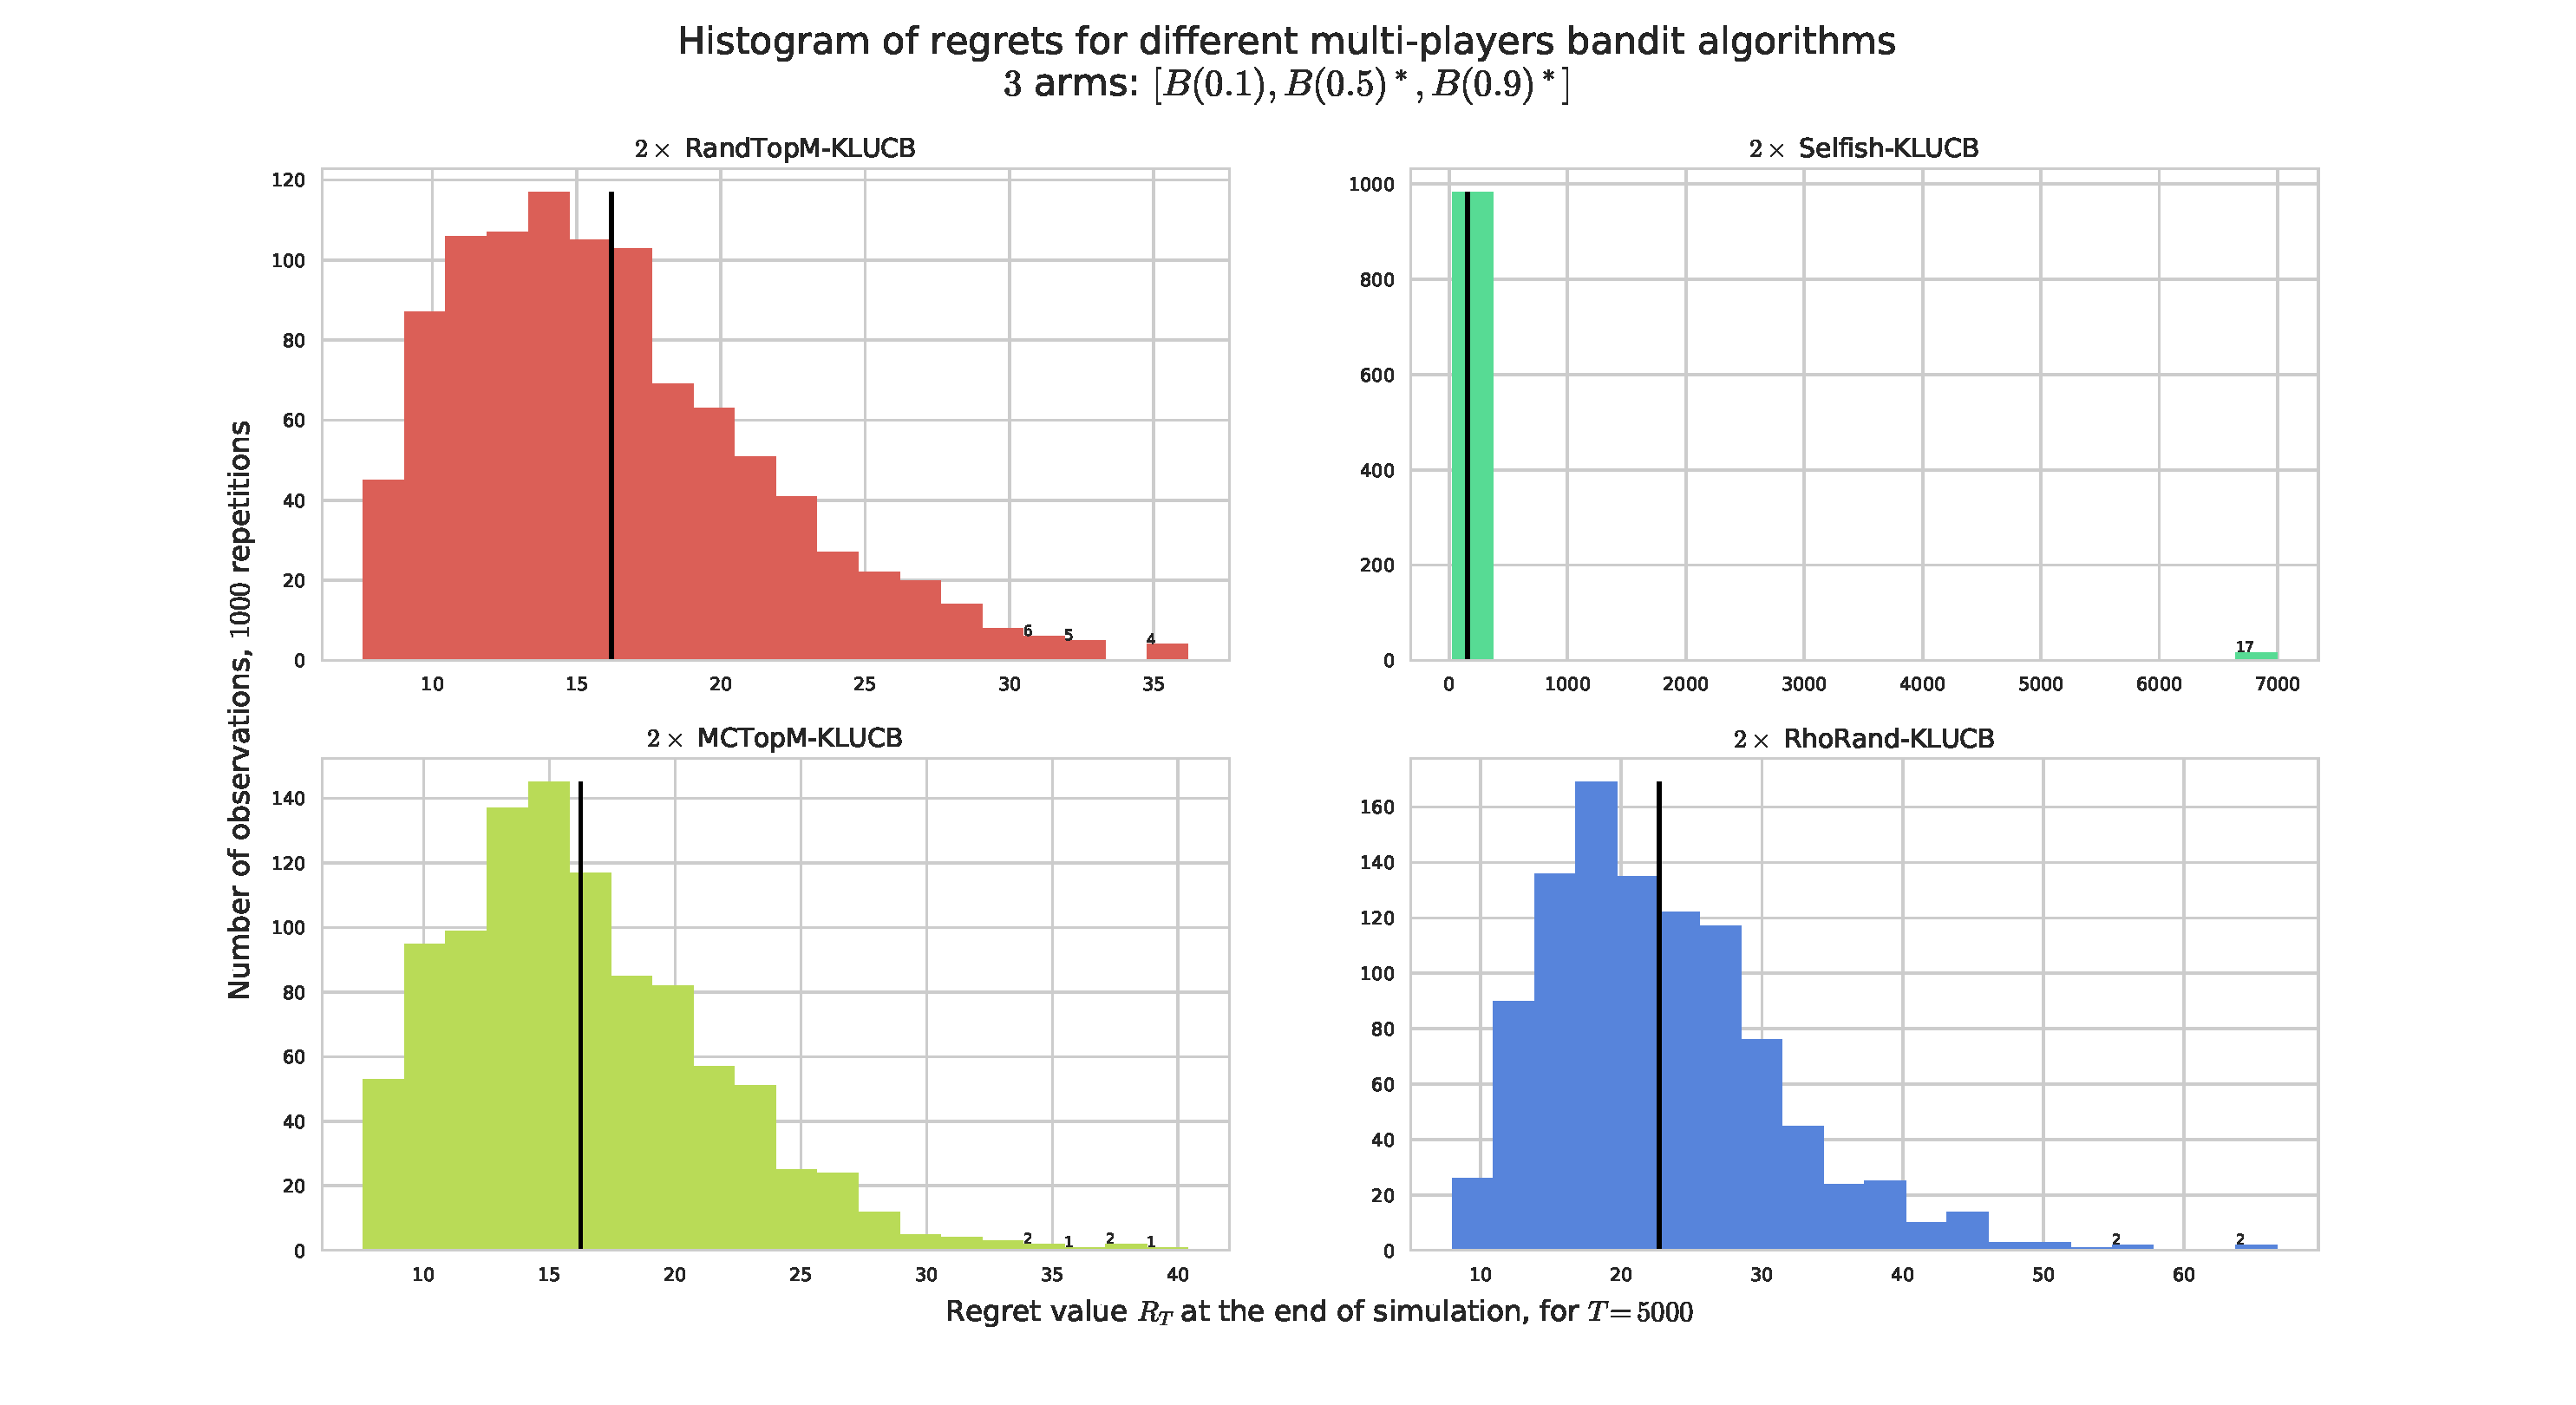
\includegraphics[width=1.10\textwidth]{MP__K3_M2_T5000_N1000__4_algos/all_HistogramsRegret____env1-1_5016720151160452442.pdf}
  % \end{subfigure}
  % % ~
  % \begin{subfigure}[!h]{0.49\textwidth}
  %   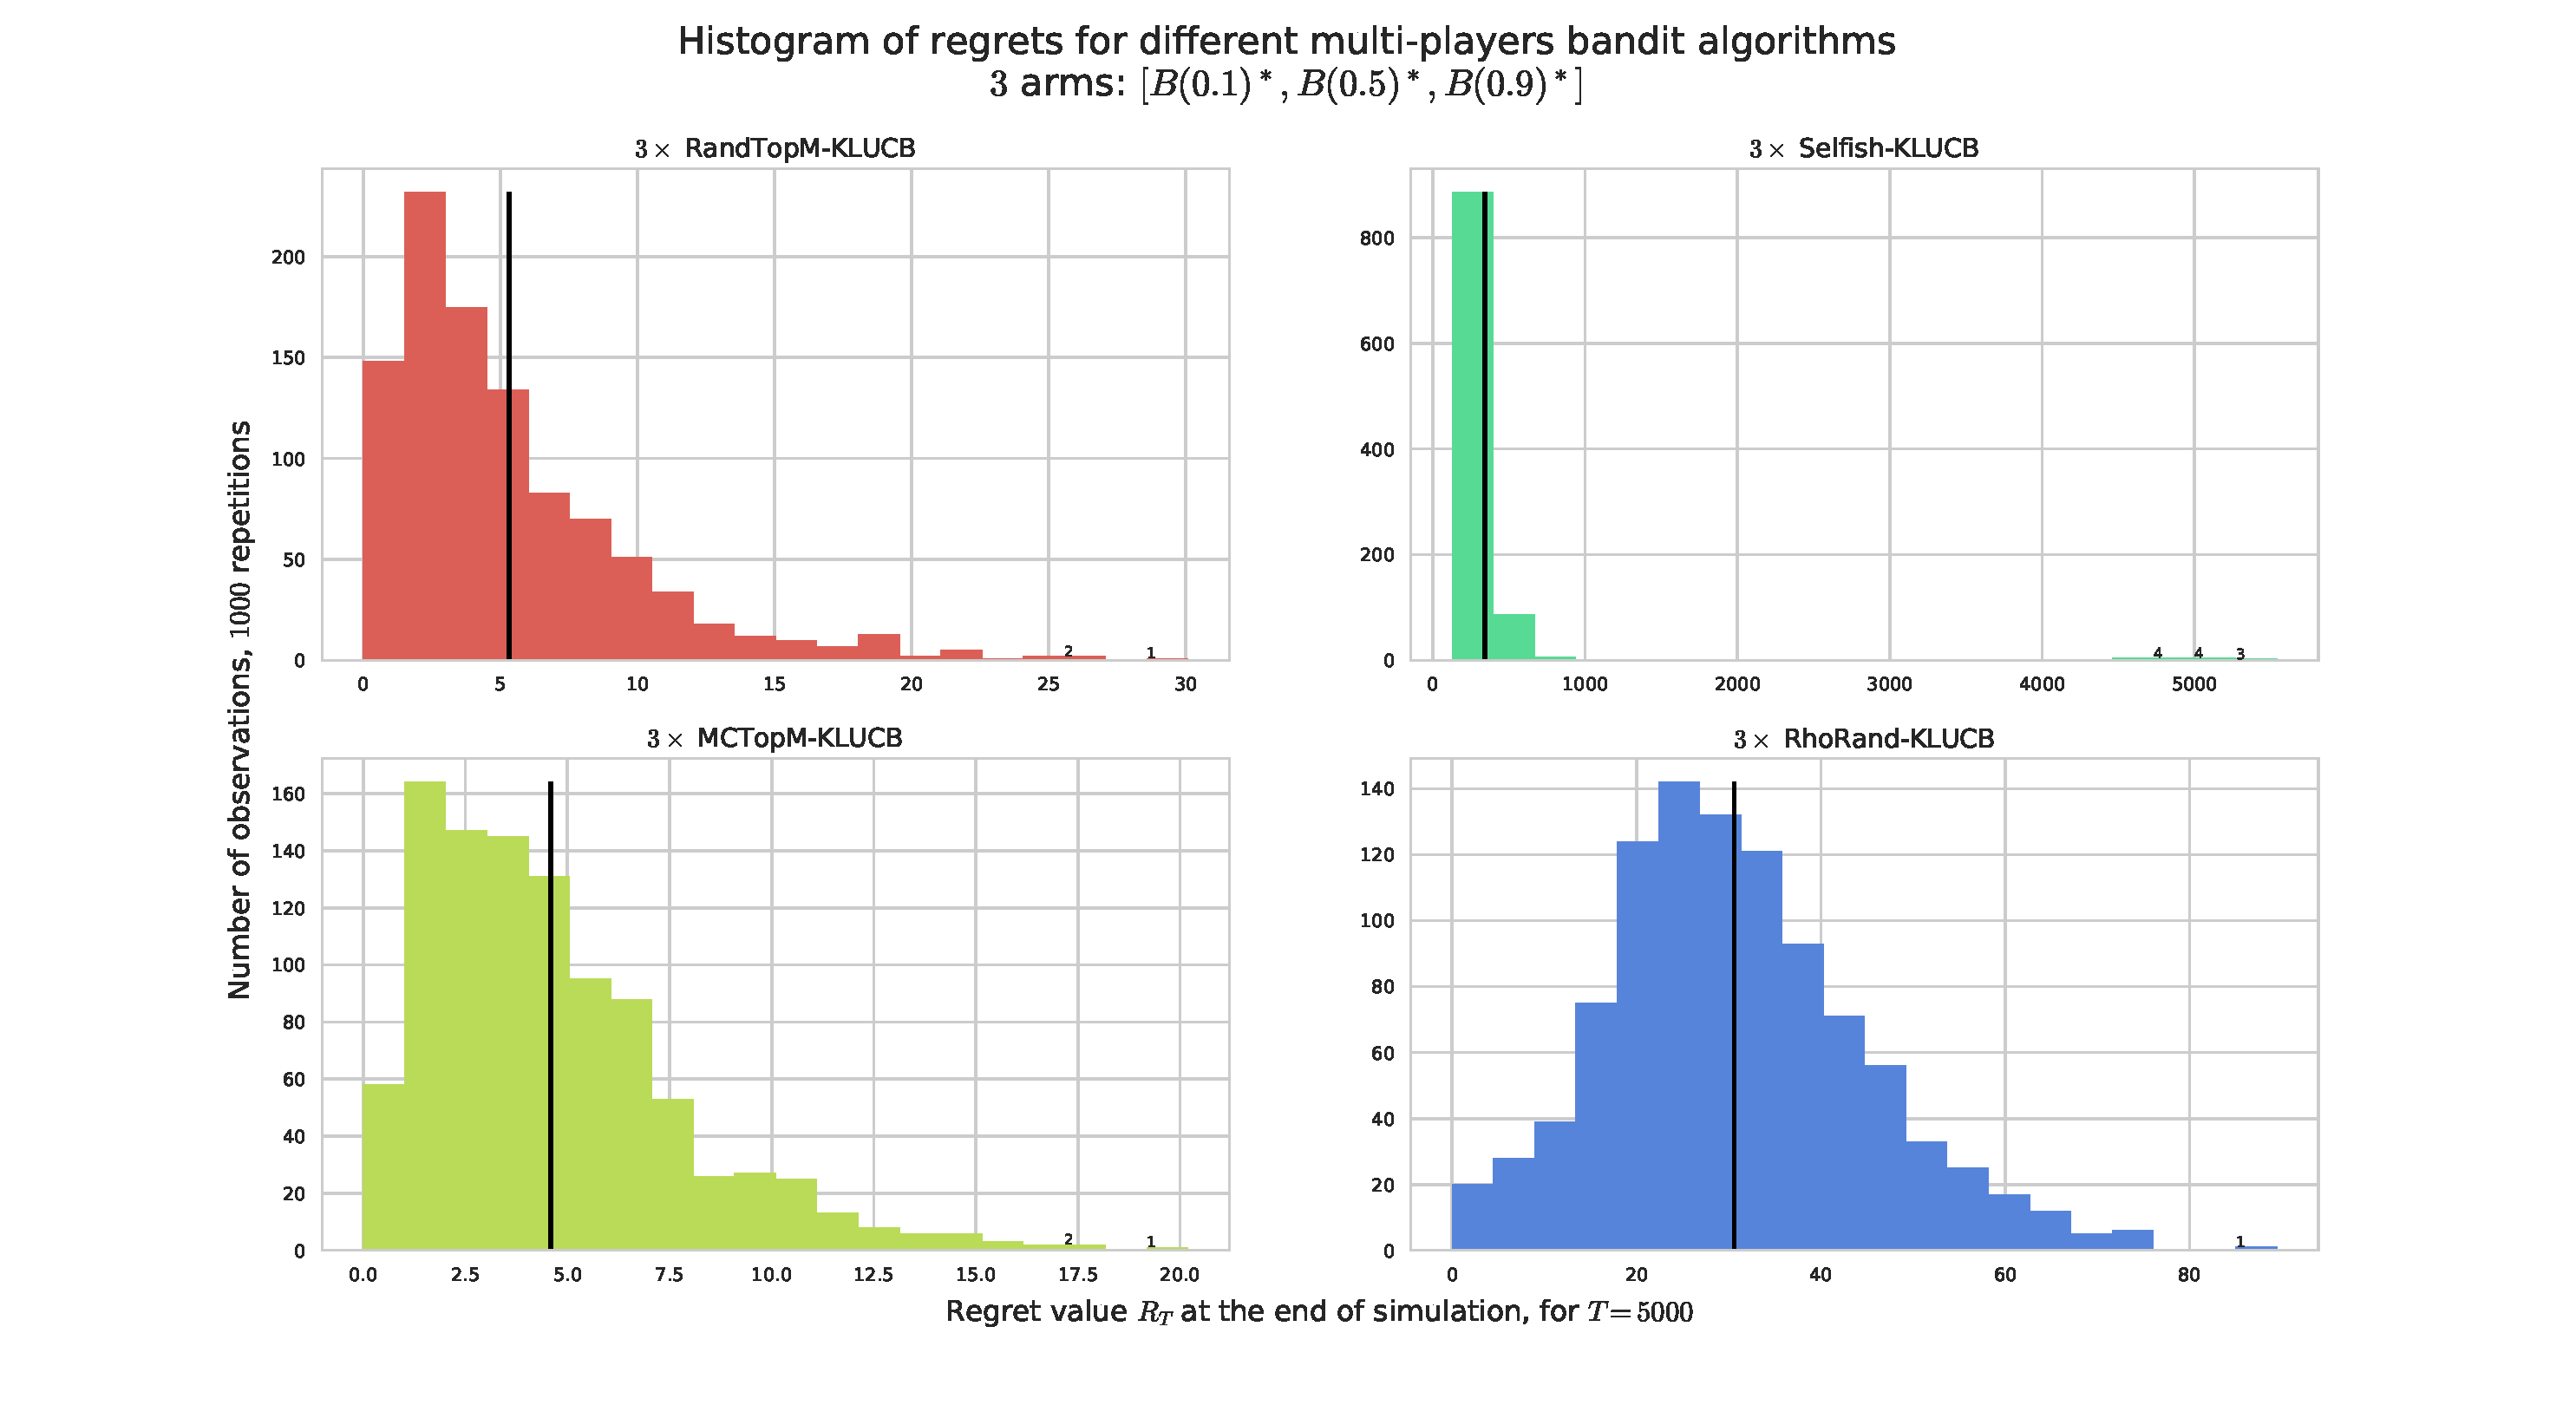
\includegraphics[width=1.10\textwidth]{MP__K3_M3_T5000_N1000__4_algos/all_HistogramsRegret____env1-1_1035303196230283176.pdf}
  % \end{subfigure}
  \caption[Failure case of \Selfish.]{Regret for $M=2$ players, $K=3$ arms, horizon $T=5000$, $1000$ repetitions and $\boldsymbol{\mu} = [0.1, 0.5, 0.9]$. Axis $x$ is for regret (different scale for each part), and the \textcolor{darkgreen}{green curve for \Selfish} shows a small probability of having a linear regret ($17$ cases of $R_T \geq T$, out of $1000$). The regret for the three other algorithms is very small for this problem, always smaller than $100$ here.}
  \label{fig:5:selfish_fail1}
  % \vspace*{-15pt}  % XXX remove if problem
\end{figure}

% %
% % Regular plots of centralized regrets
% %
% \begin{figure}[!t]
%   \centering
%   % \begin{subfigure}[!h]{1.00\textwidth}
%       % 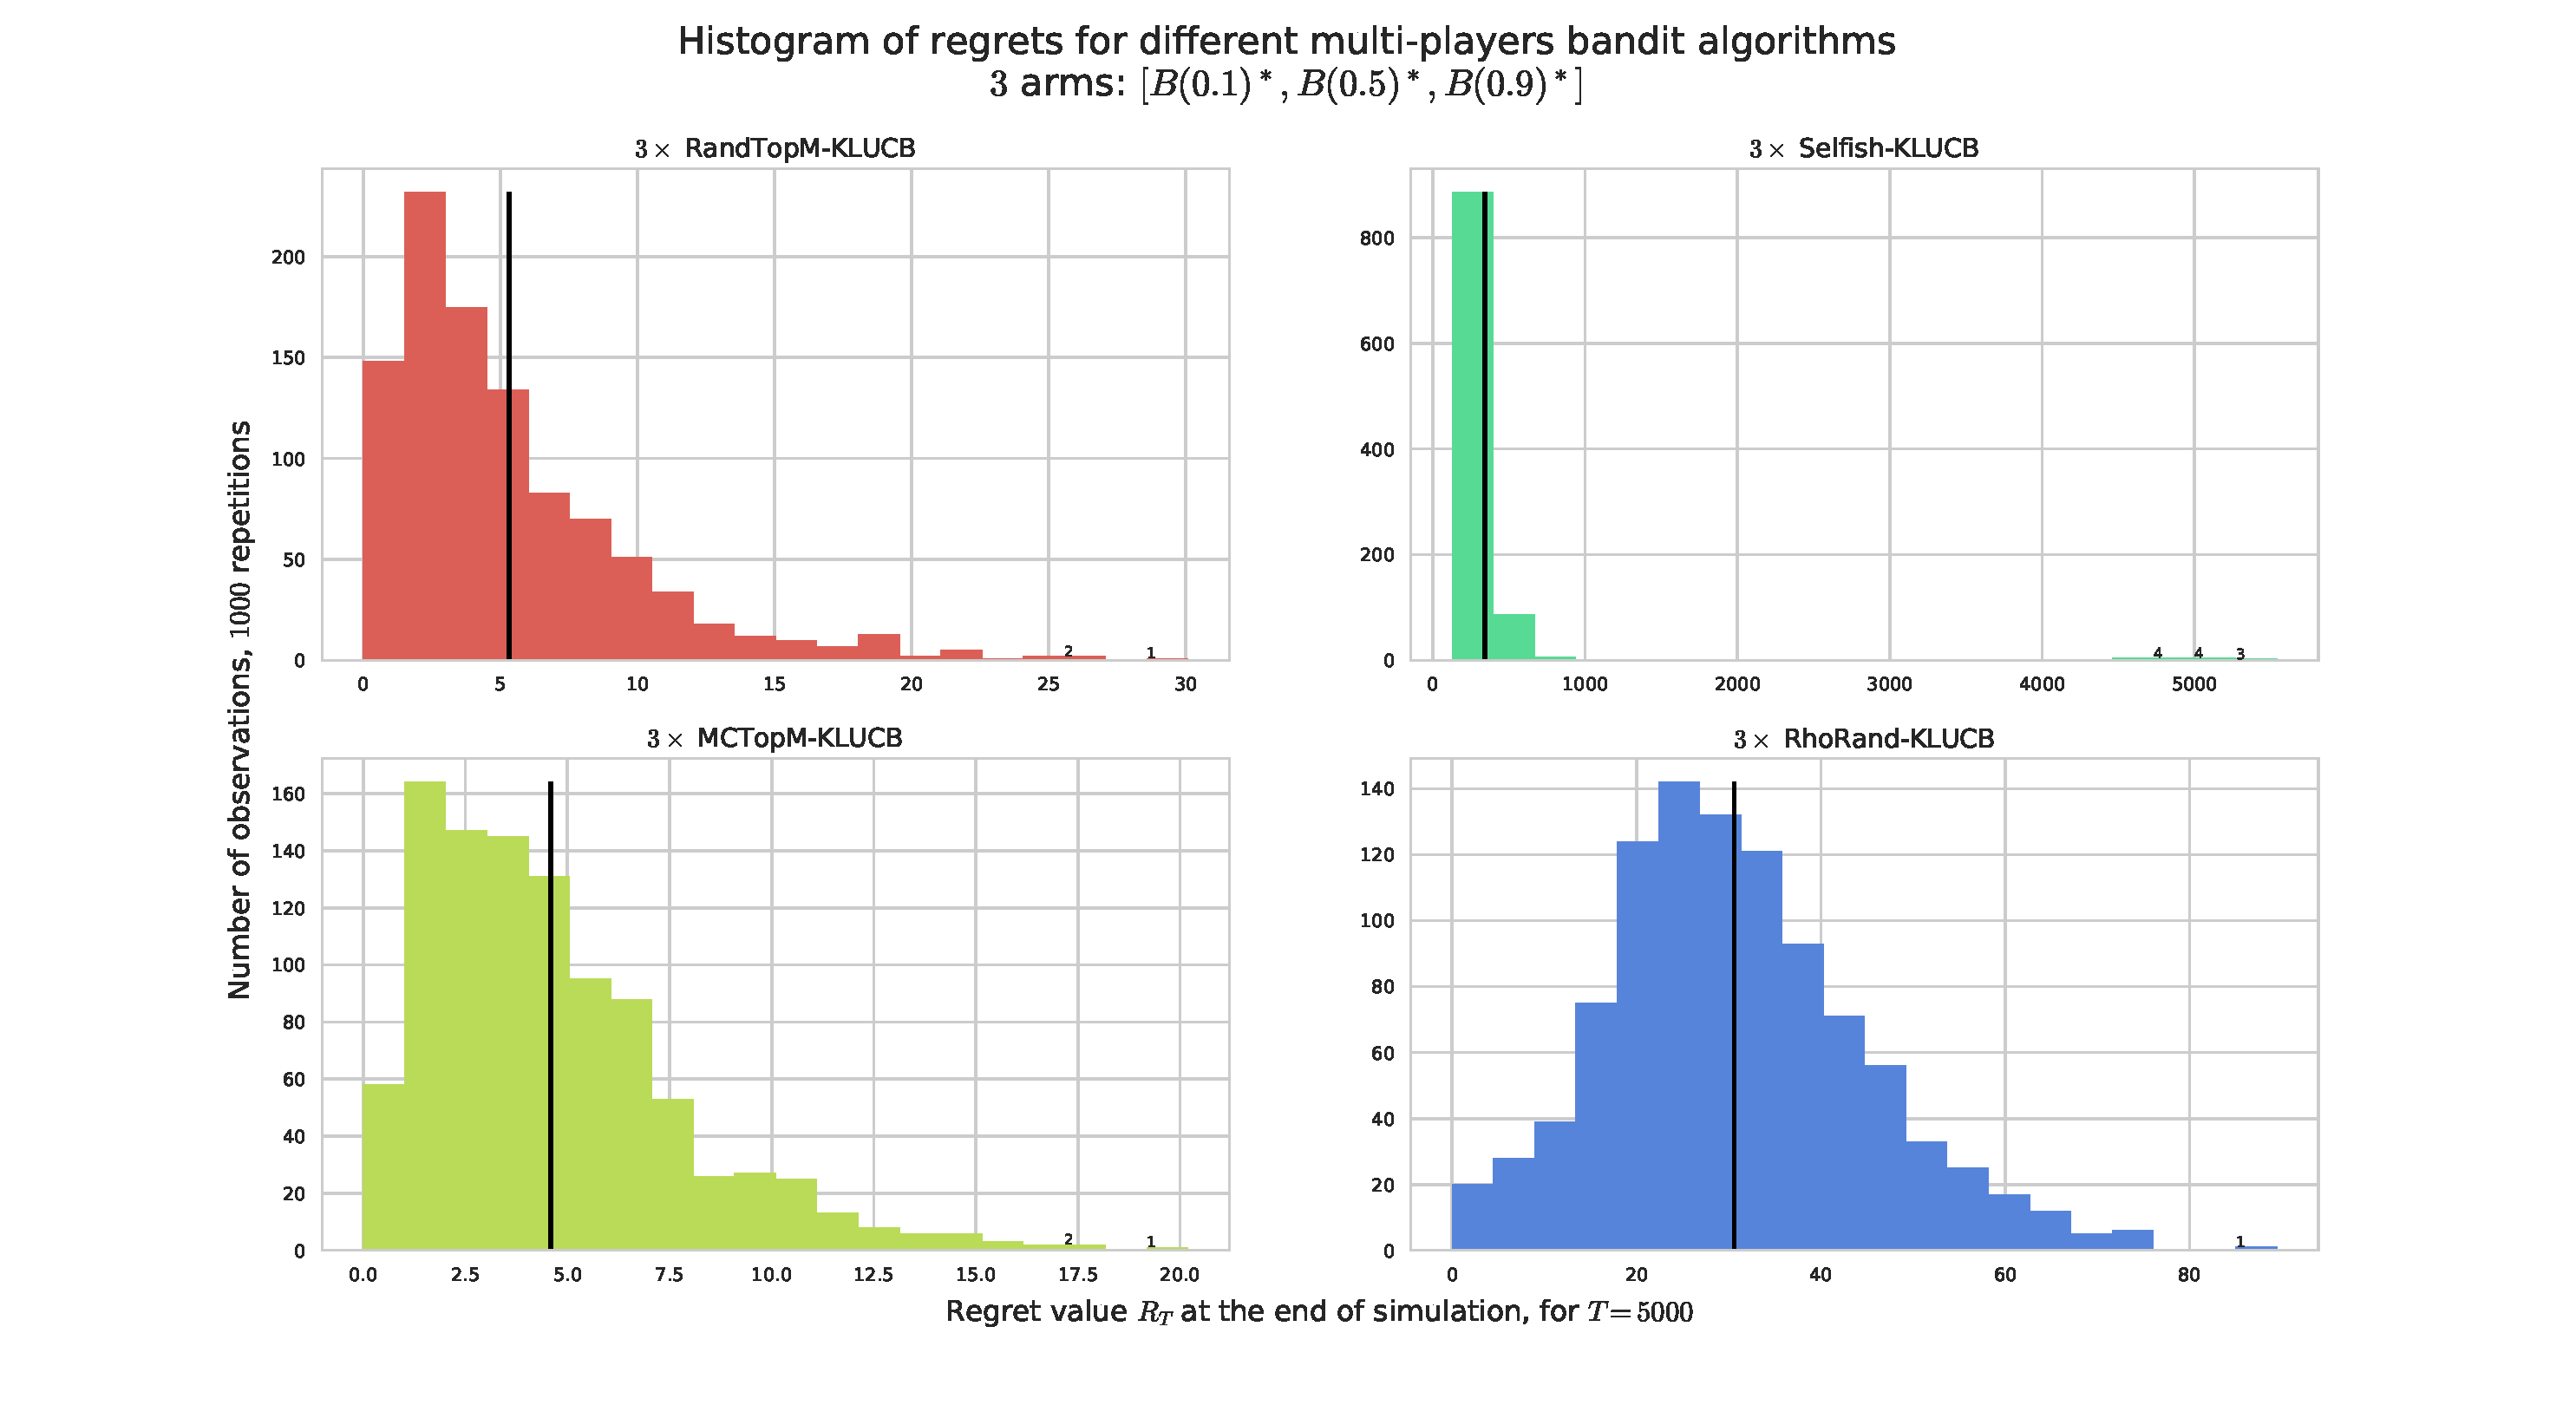
\includegraphics[width=1.00\textwidth]{MP__K3_M3_T5000_N1000__4_algos/all_HistogramsRegret____env1-1_1035303196230283176.pdf}
%       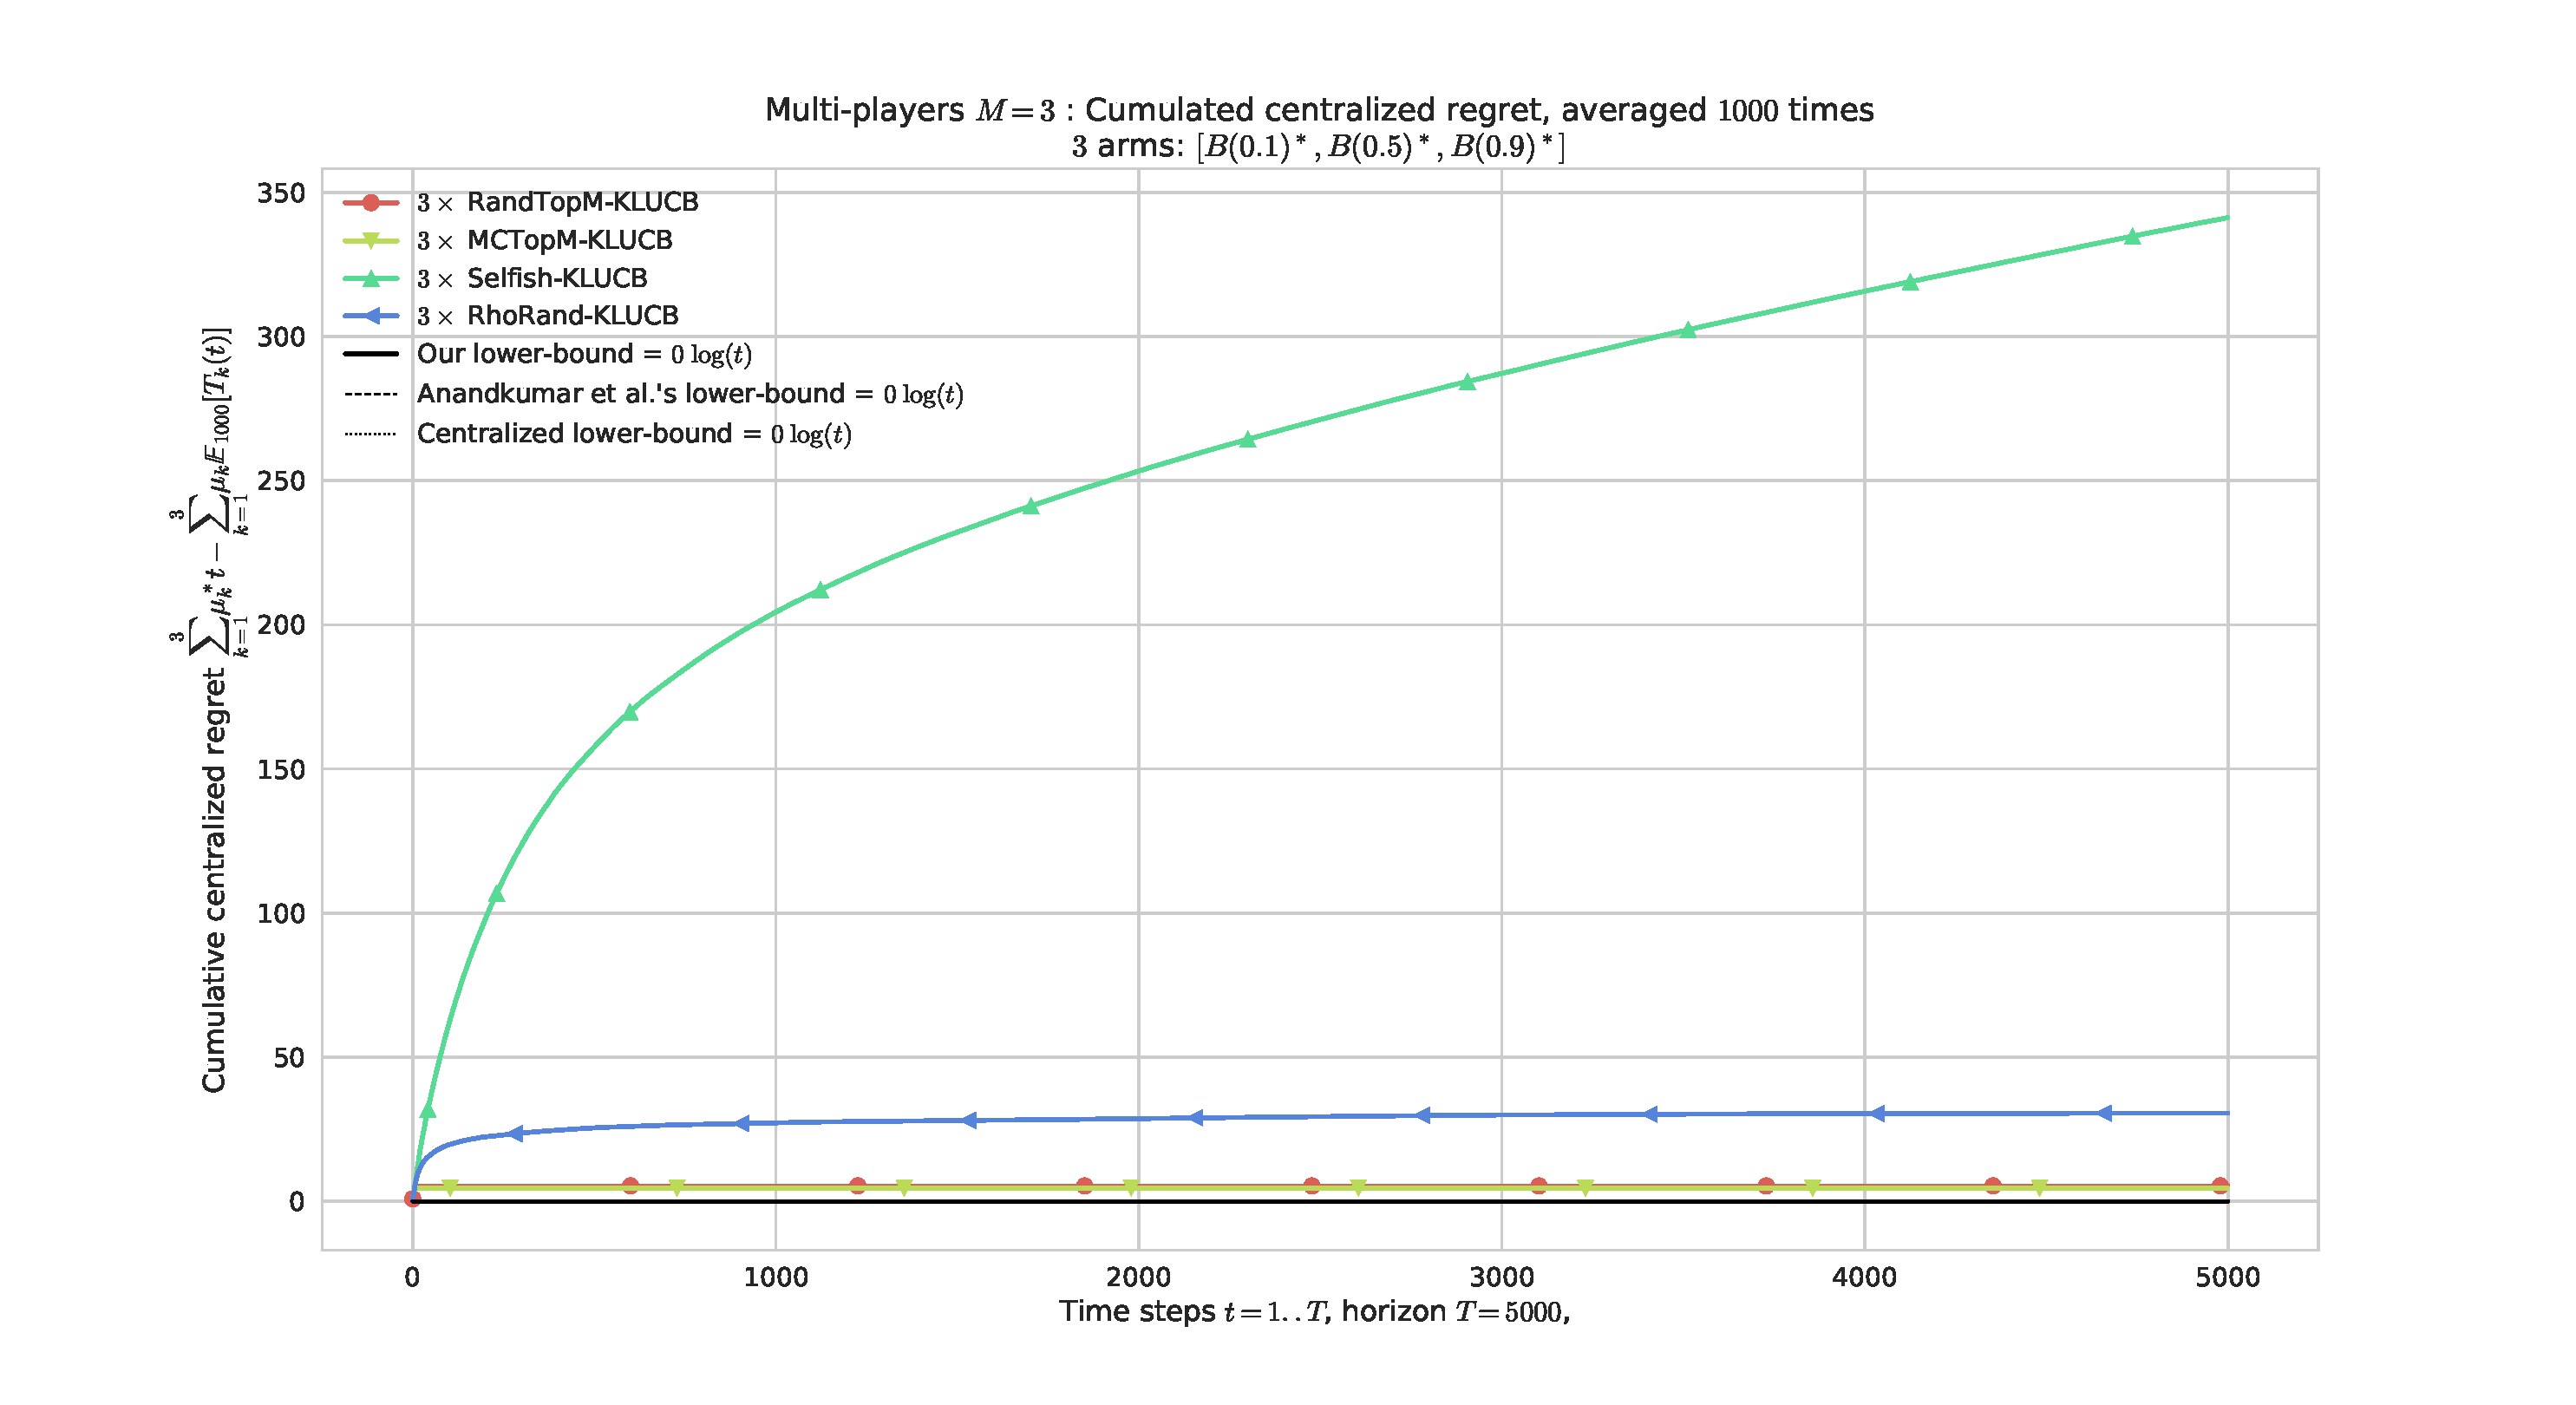
\includegraphics[width=1.00\textwidth]{MP__K3_M3_T5000_N1000__4_algos/all_RegretCentralized____env1-1_1035303196230283176.pdf}
%       % 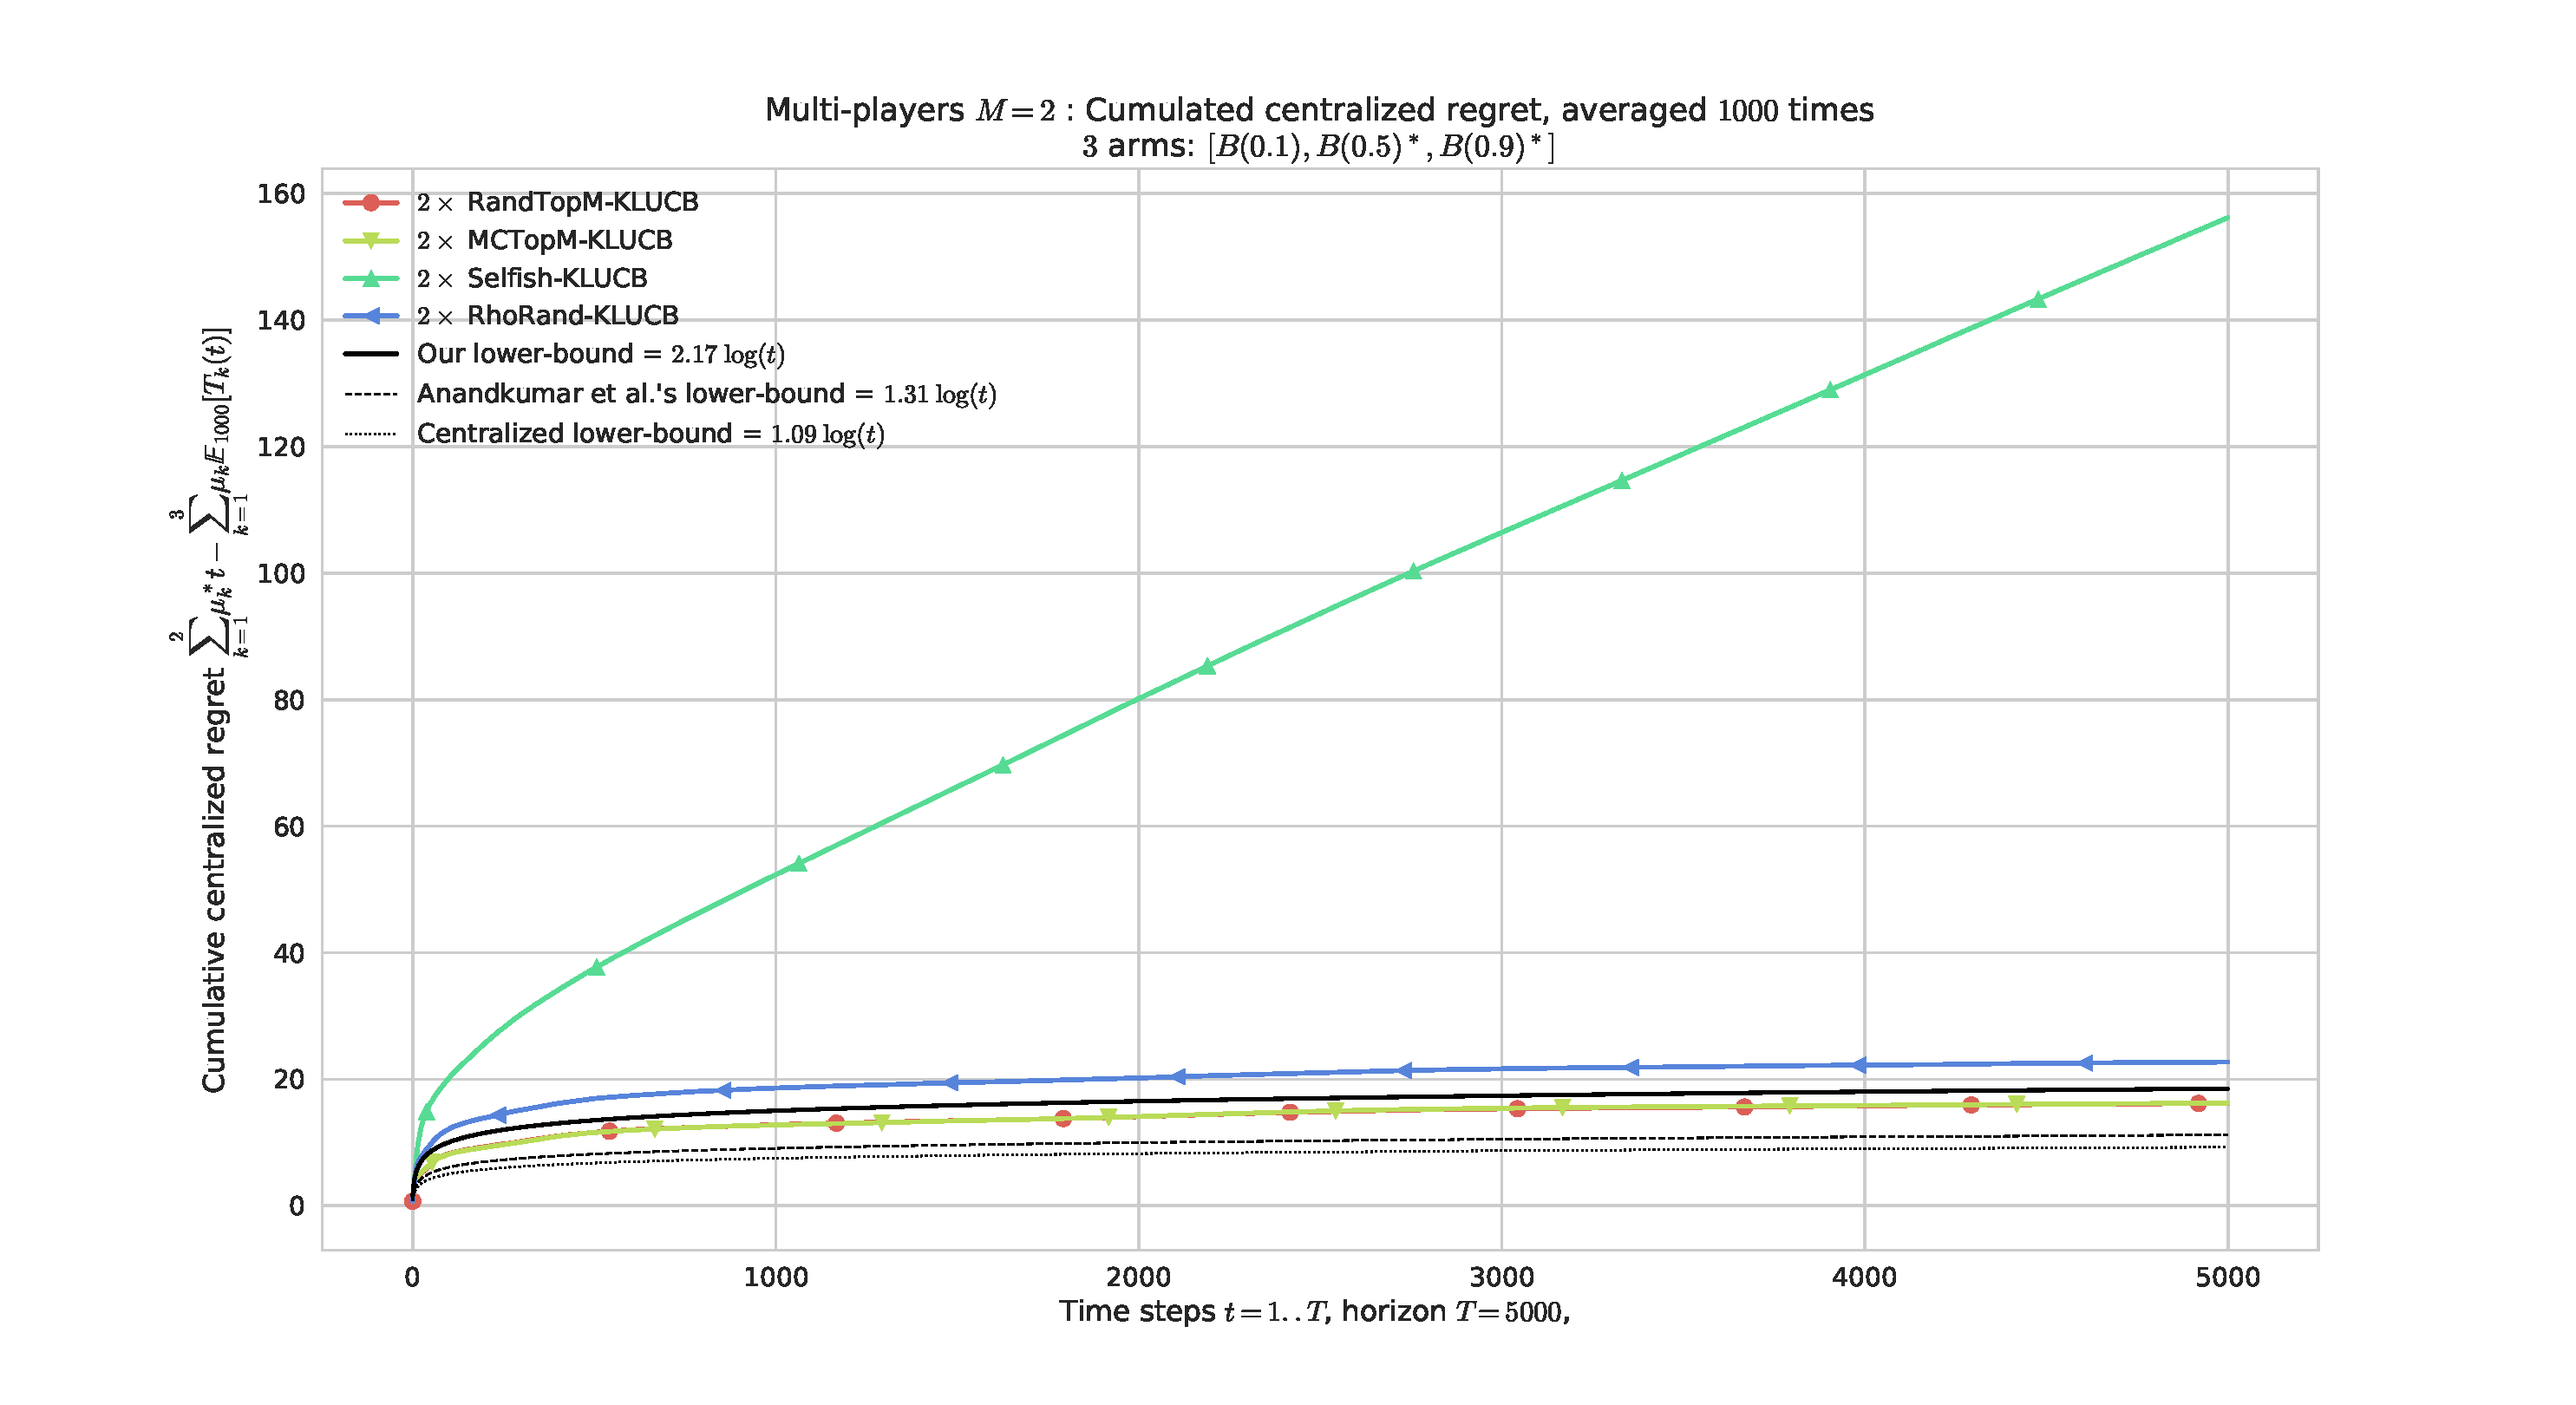
\includegraphics[width=1.00\textwidth]{MP__K3_M2_T5000_N1000__4_algos/all_RegretCentralized____env1-1_5016720151160452442.pdf}
%   % \end{subfigure}
%   ~
%   % \begin{subfigure}[!h]{1.00\textwidth}
%       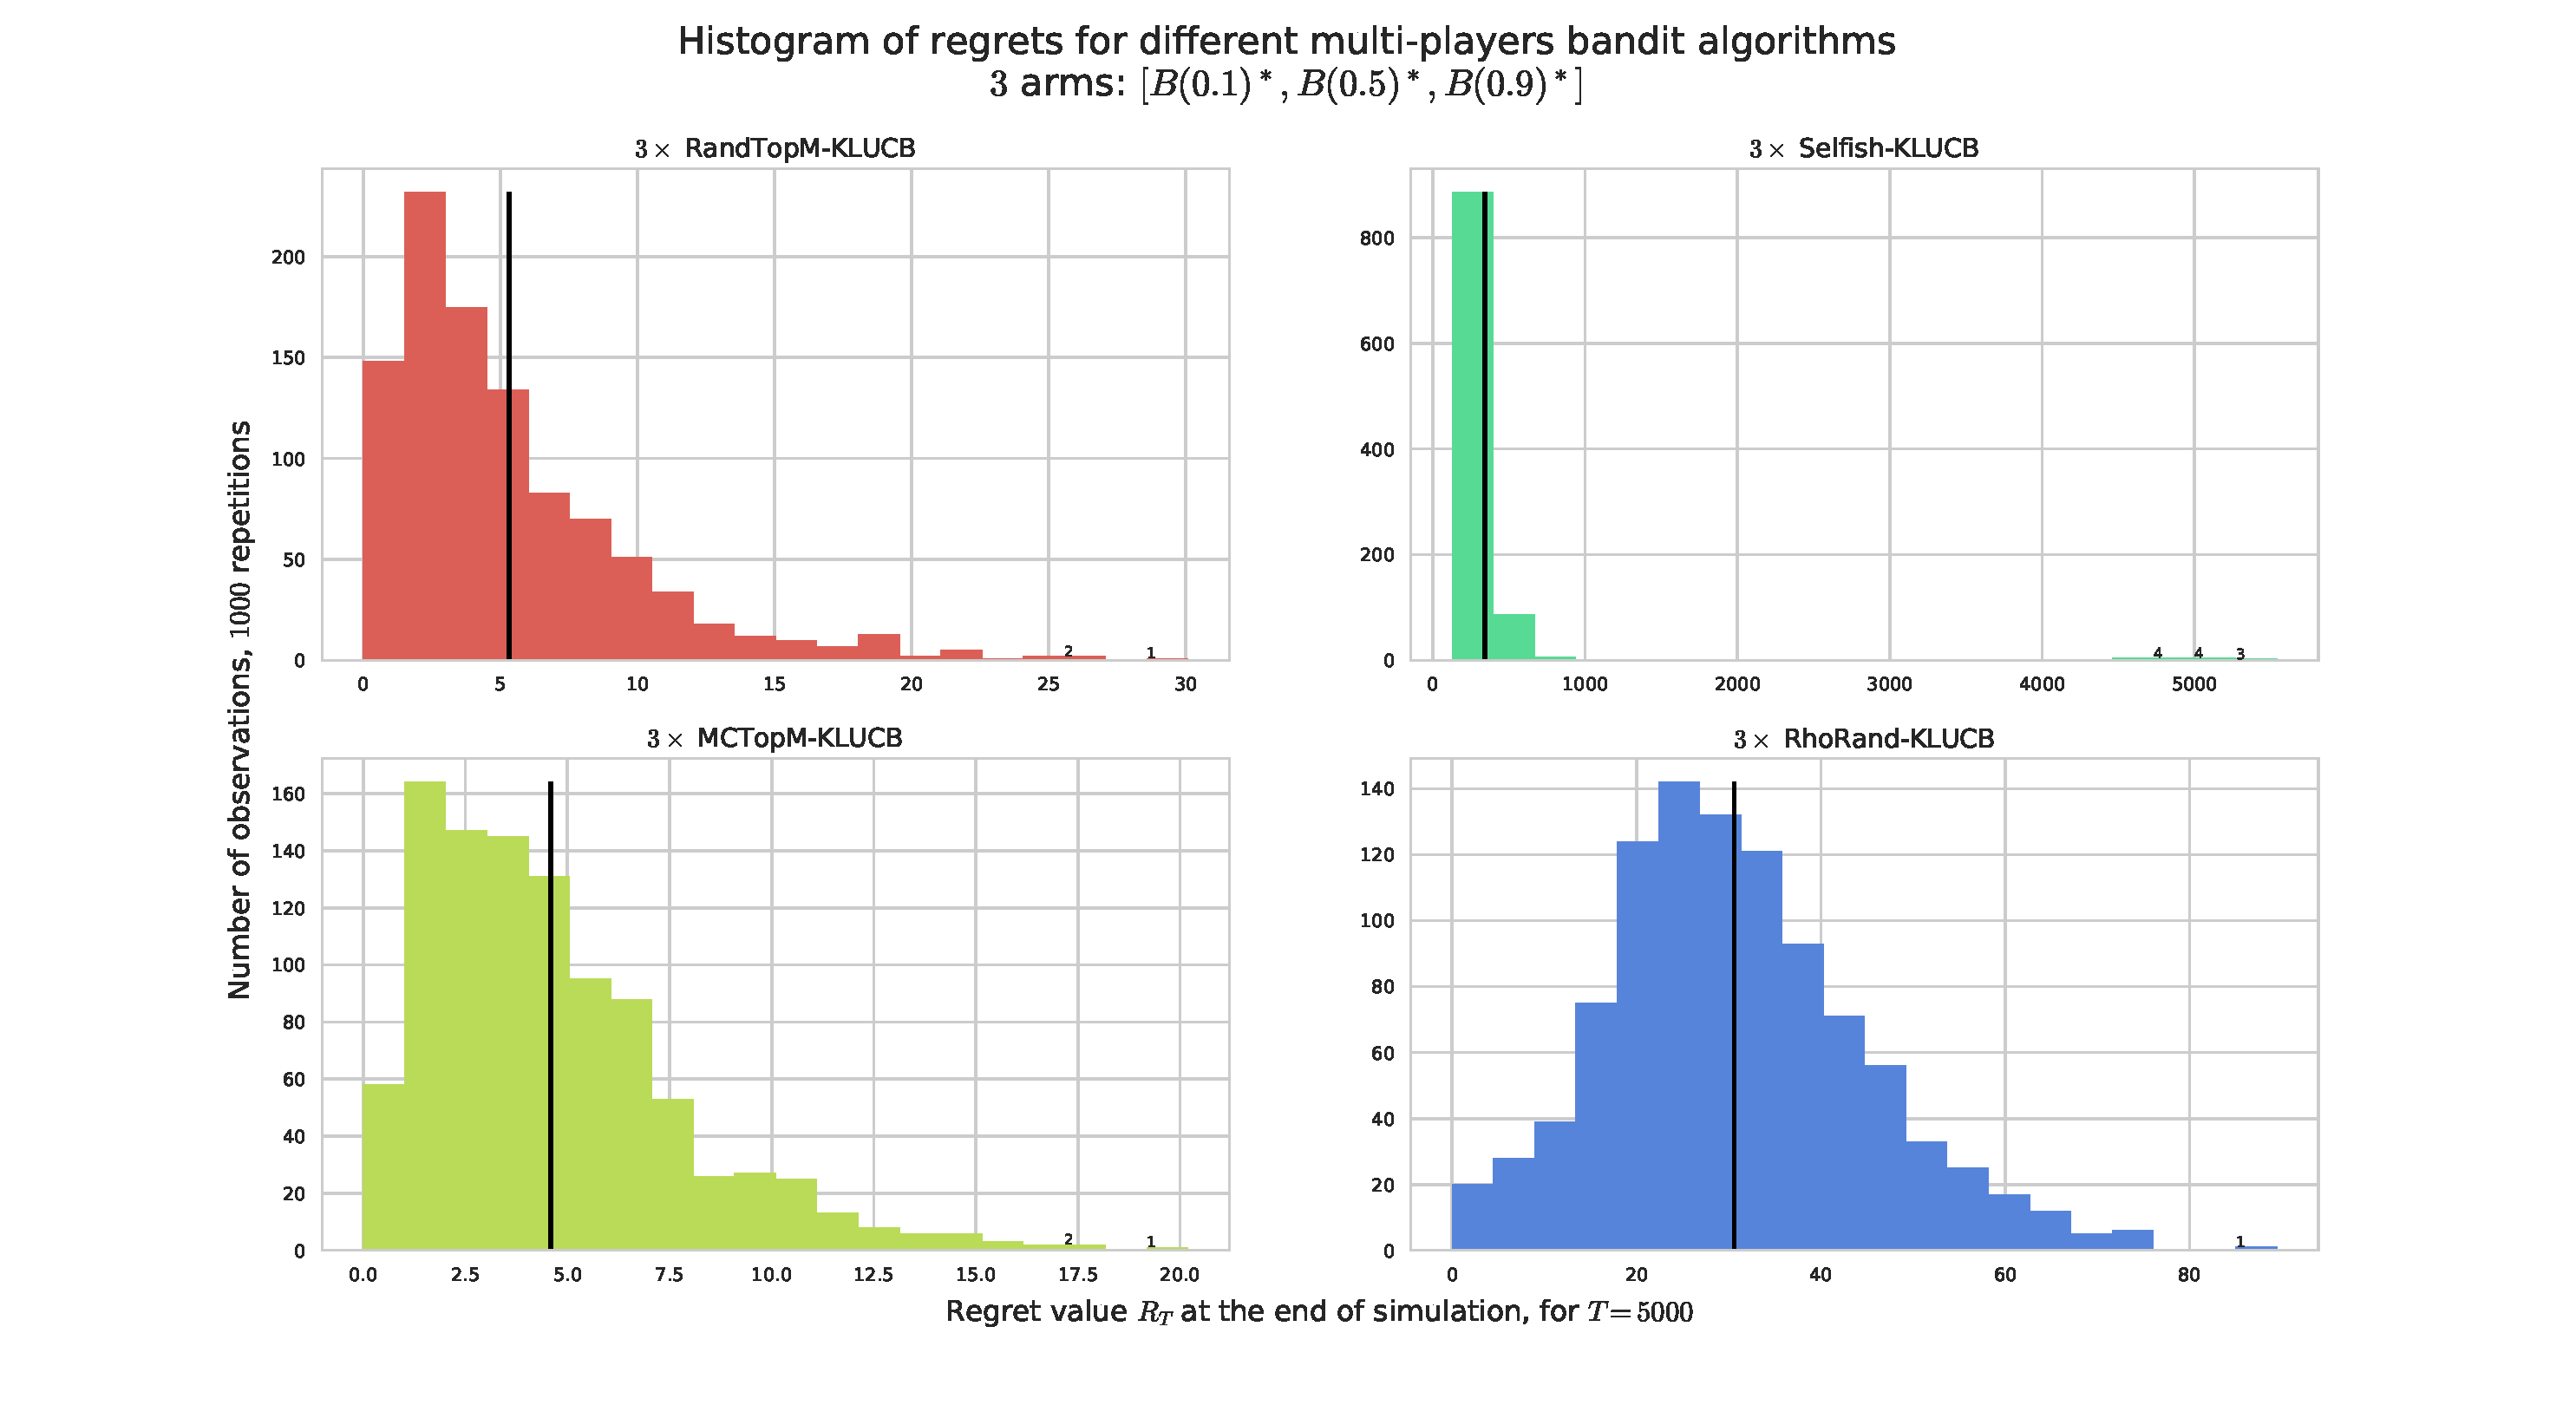
\includegraphics[width=1.00\textwidth]{MP__K3_M3_T5000_N1000__4_algos/all_HistogramsRegret____env1-1_1035303196230283176.pdf}
%   % \end{subfigure}
%   \caption[Third failure case of \Selfish]{Regret for $M=3$ players, $K=3$ arms, horizon $T=5000$, $1000$ repetitions and $\boldsymbol{\mu} = [0.1, 0.5, 0.9]$. Axis $x$ is for regret (different scale for each), and the top \textcolor{darkgreen}{green} curve for \Selfish{} shows a small probability of having a linear regret ($11$ cases of $R_T \geq T$, out of $1000$). The regret for the three other algorithms is very small for this problem, and even appears constant.}
%   \label{fig:5:selfish_fail3}
%   % \vspace*{-15pt}  % XXX remove if problem
% \end{figure}


\begin{figure}[!b]
  \centering
  % \begin{subfigure}[!h]{0.85\textwidth}
    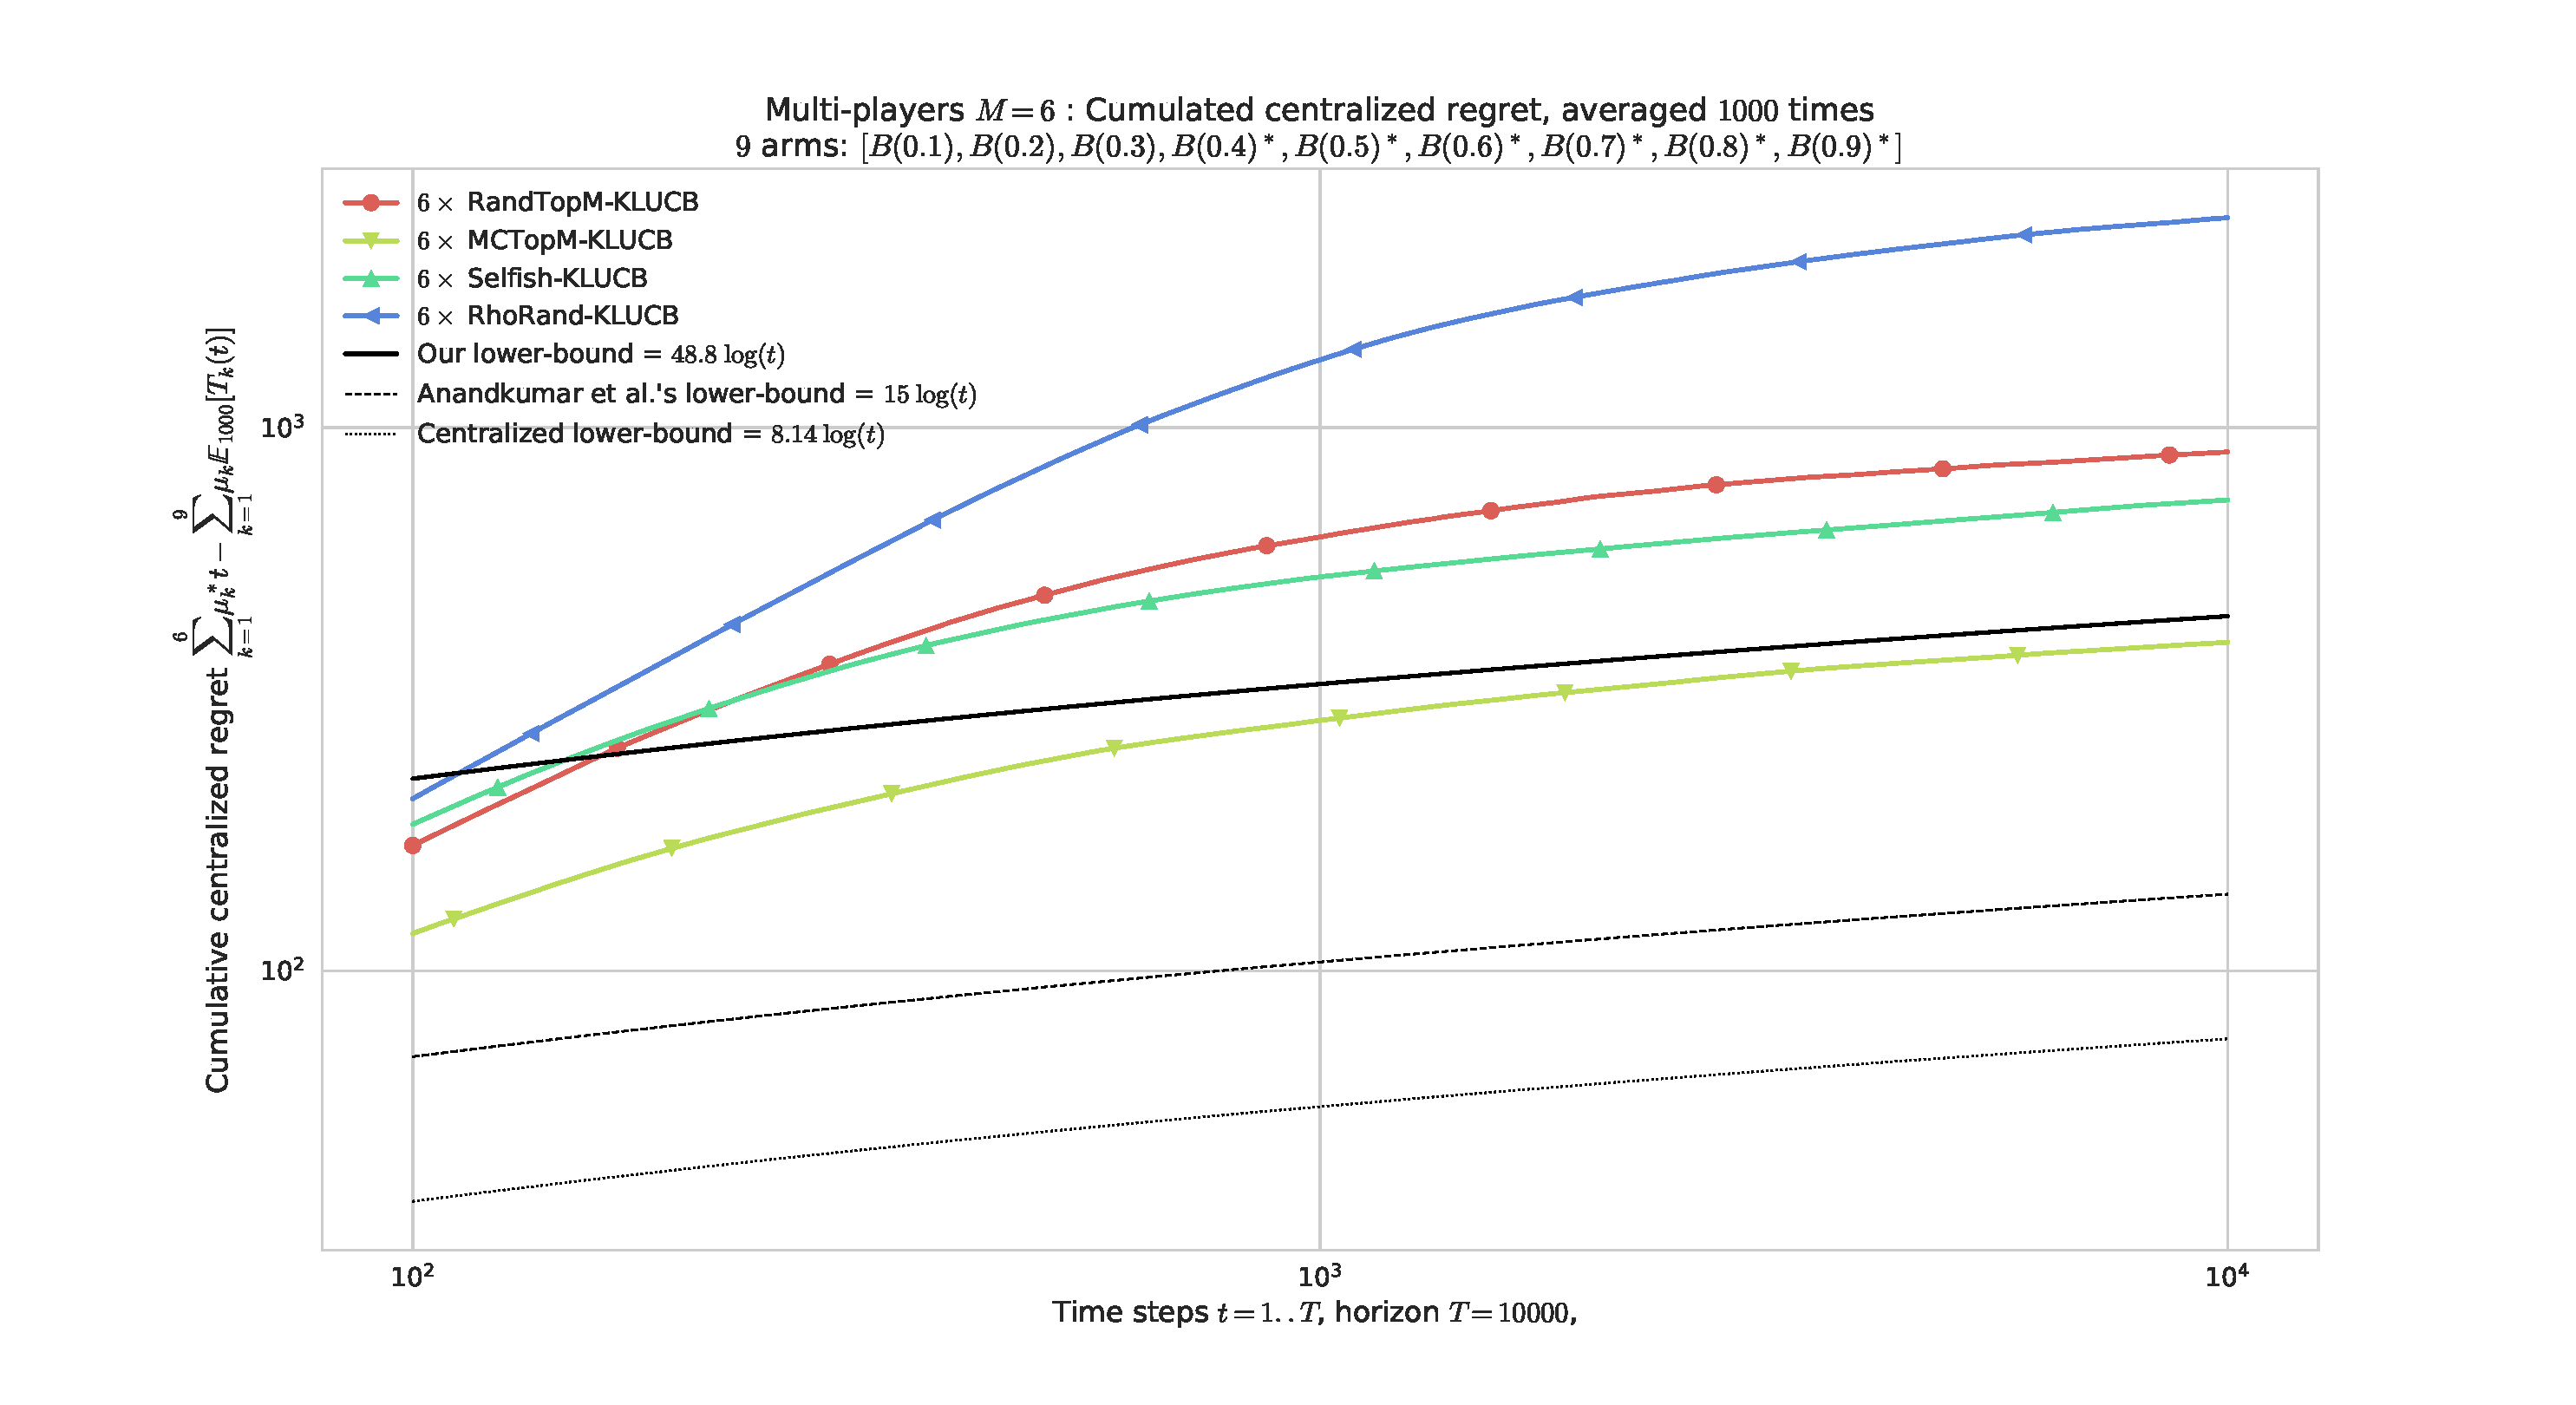
\includegraphics[width=1.10\textwidth]{MP__K9_M6_T10000_N1000__4_algos/all_RegretCentralized_loglog____env1-1_8200873569864822246.pdf}
  % \end{subfigure}
  % ~
  % \begin{subfigure}[!h]{0.85\textwidth}
    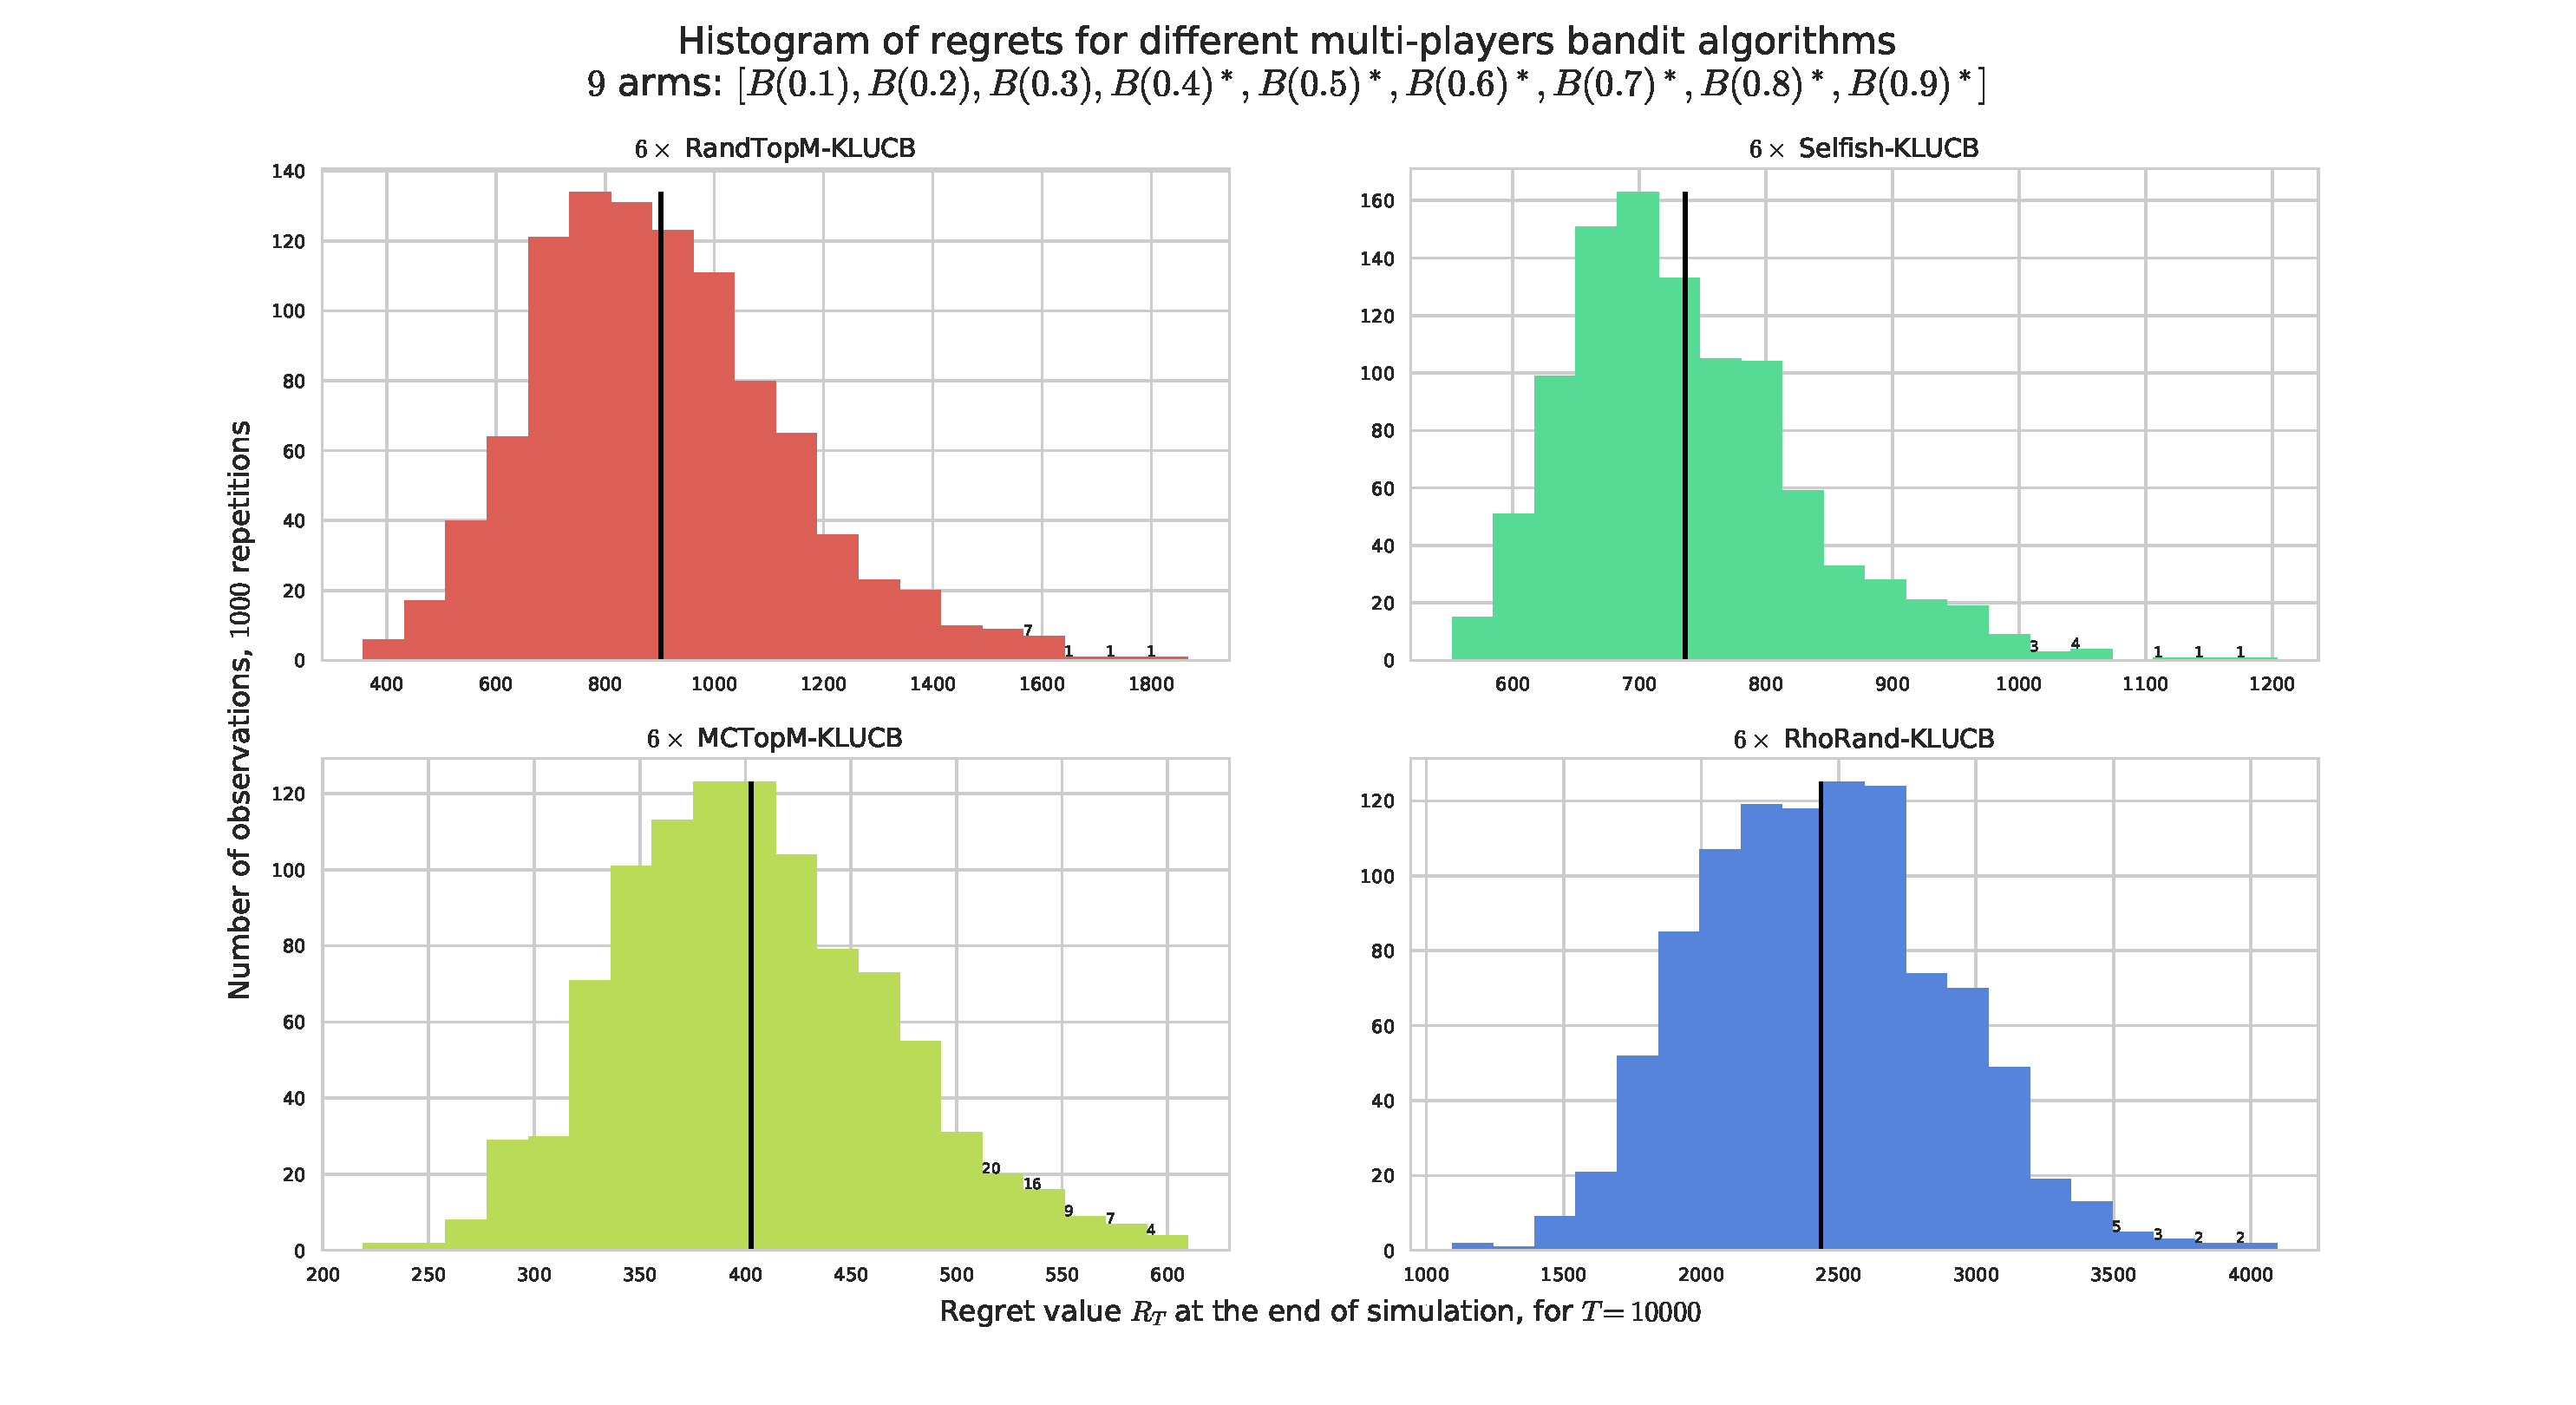
\includegraphics[width=1.10\textwidth]{MP__K9_M6_T10000_N1000__4_algos/all_HistogramsRegret____env1-1_8200873569864822246.pdf}
  % \end{subfigure}
  \caption[Regret for $M=6$ players for $K=9$ arms, horizon $T=5000$, for $1000$ repetitions on a fixed problem.]{Regret (in log-log scale), for $M=6$ players for $K=9$ arms, horizon $T=5000$, for $1000$ repetitions on problem $\boldsymbol{\mu}=[0.1,\dots,0.9]$. \textcolor{lightgreen}{\RandTopM{} (in light green)} outperforms \textcolor{darkgreen}{\Selfish{} (in green)}, both clearly outperform \rhoRand. The regret of \MCTopM{} is logarithmic, empirically with the same slope as the lower bound. The $x$ axis on the regret histograms have different scale for each algorithm.}
  \label{fig:5:MP__K9_M6_T10000_N1000__4_algos}
\end{figure}


\begin{figure}[!t]
  \centering
  % \begin{subfigure}[!h]{1.00\textwidth}
      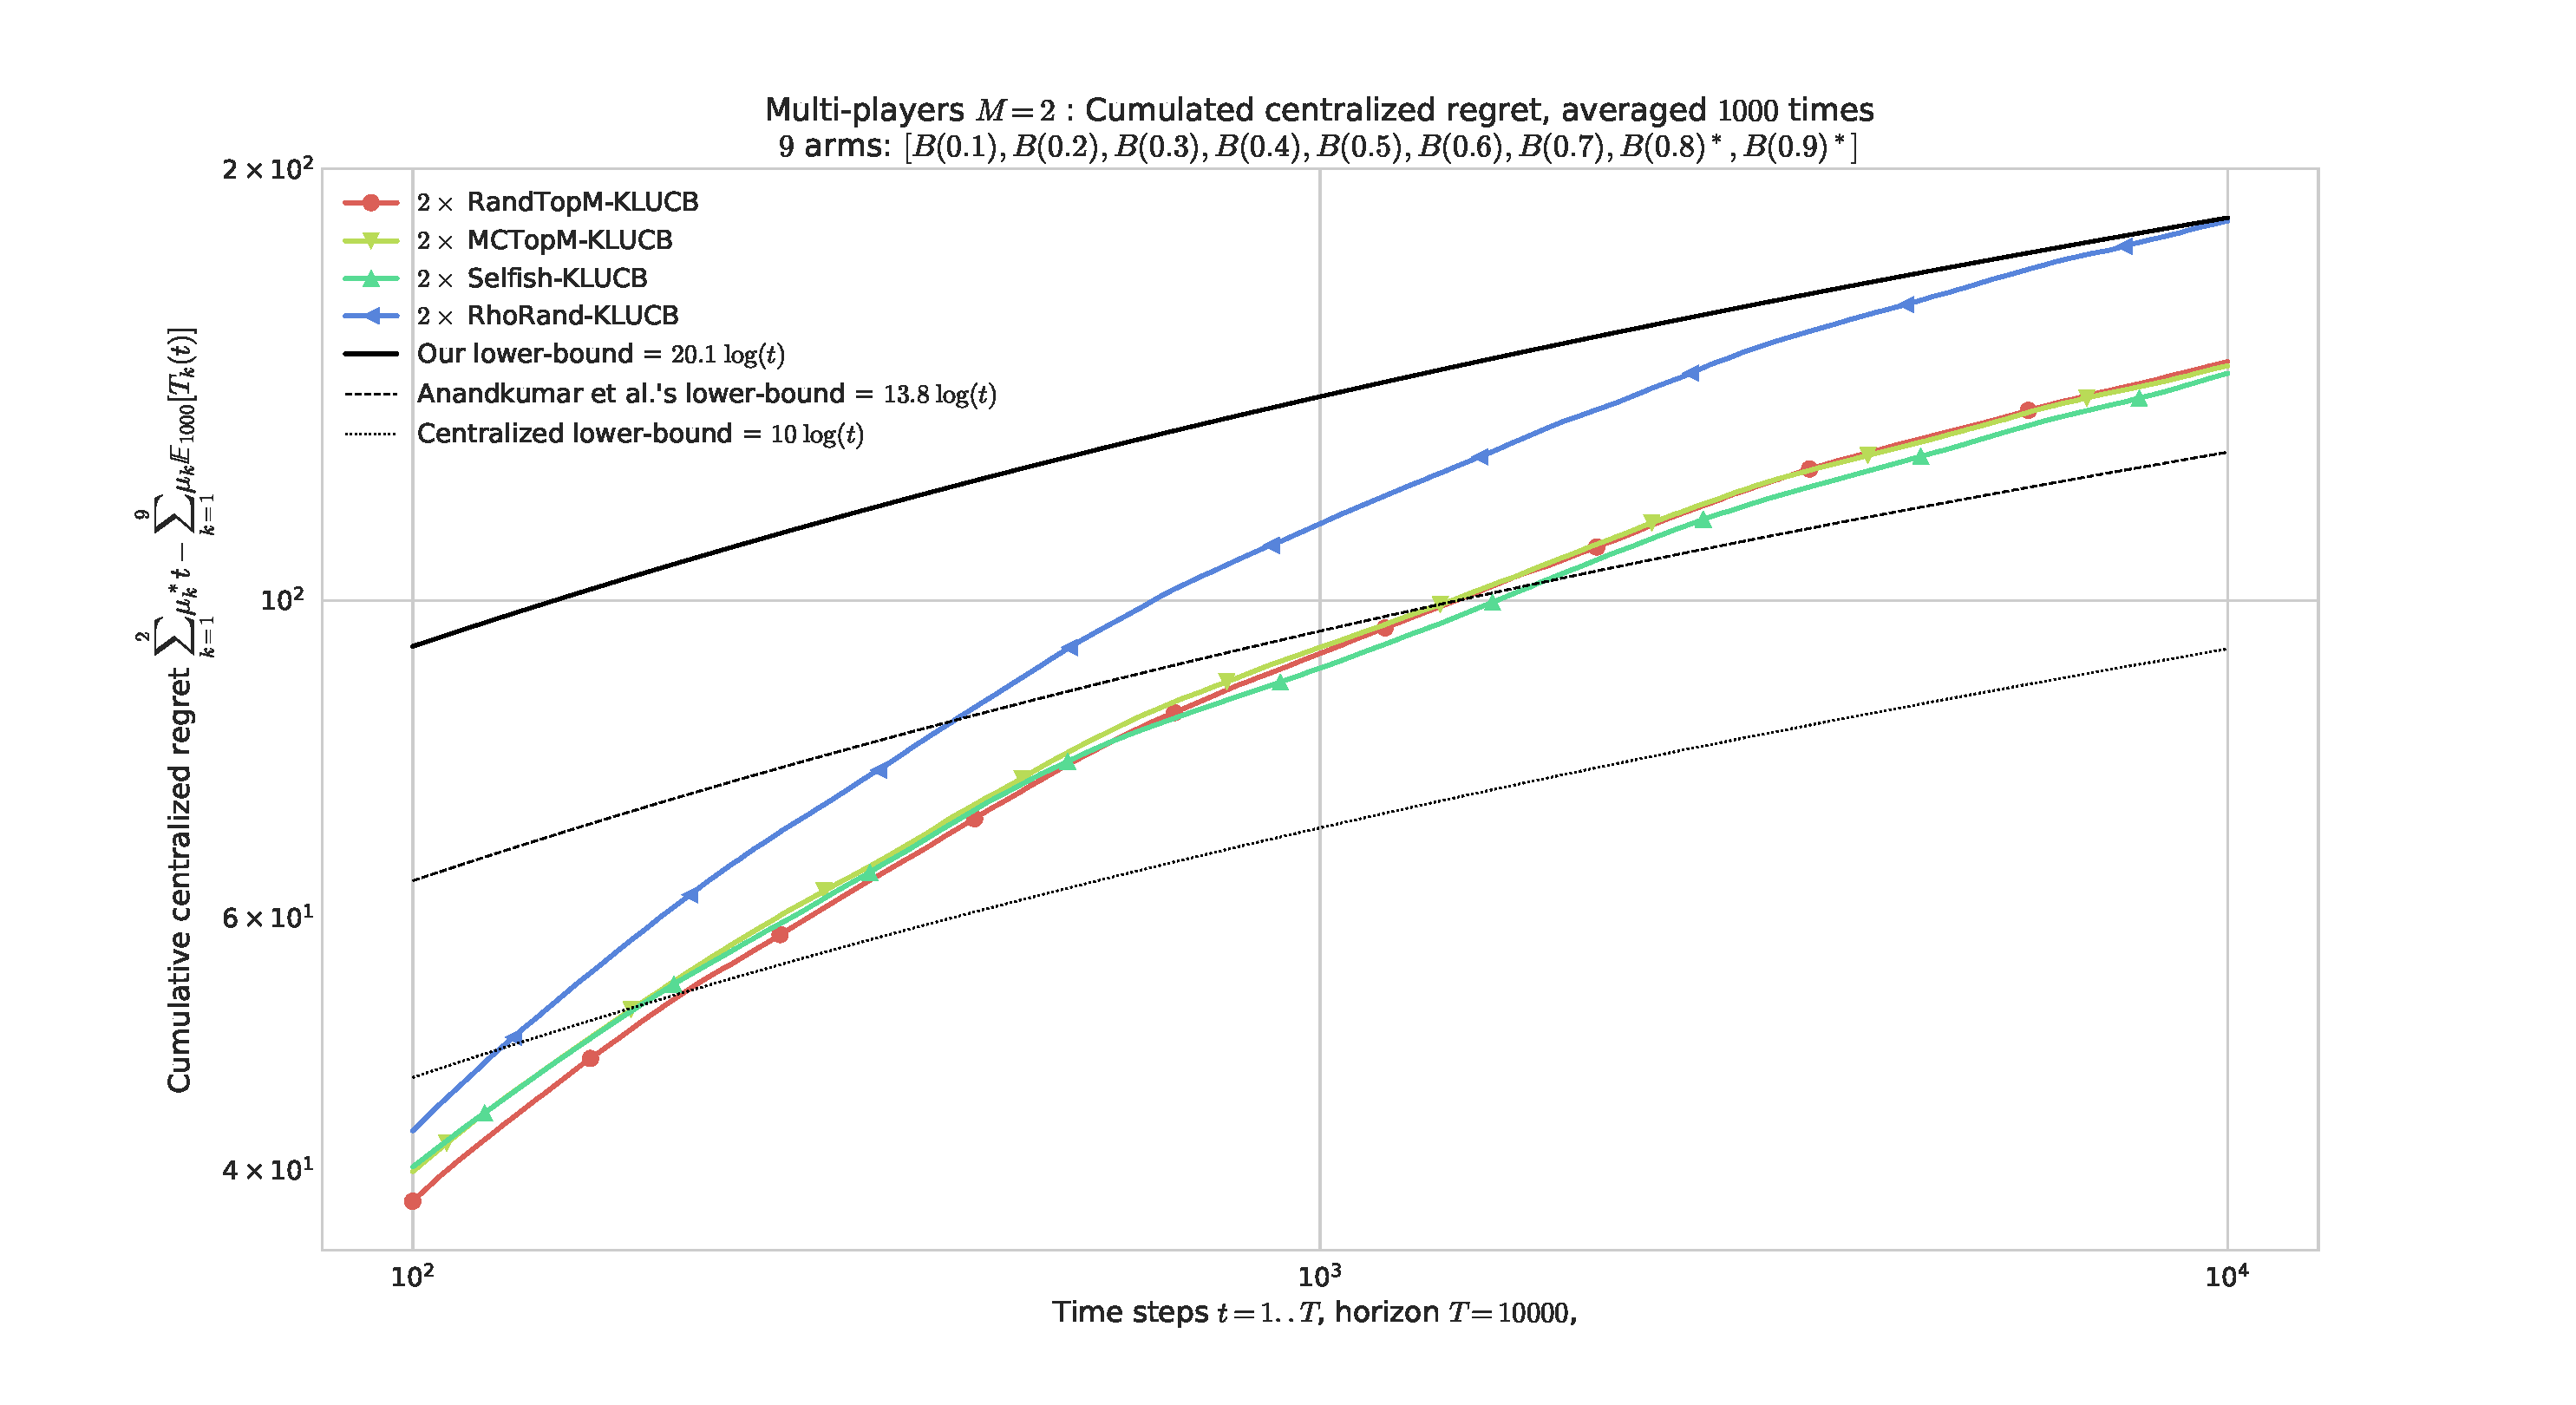
\includegraphics[width=1.10\textwidth]{MP__K9_M2_T10000_N1000__4_algos/all_RegretCentralized_loglog____env1-1_2643359116089264295.pdf}
  % \end{subfigure}
  % ~
  % \begin{subfigure}[!h]{1.00\textwidth}
  %   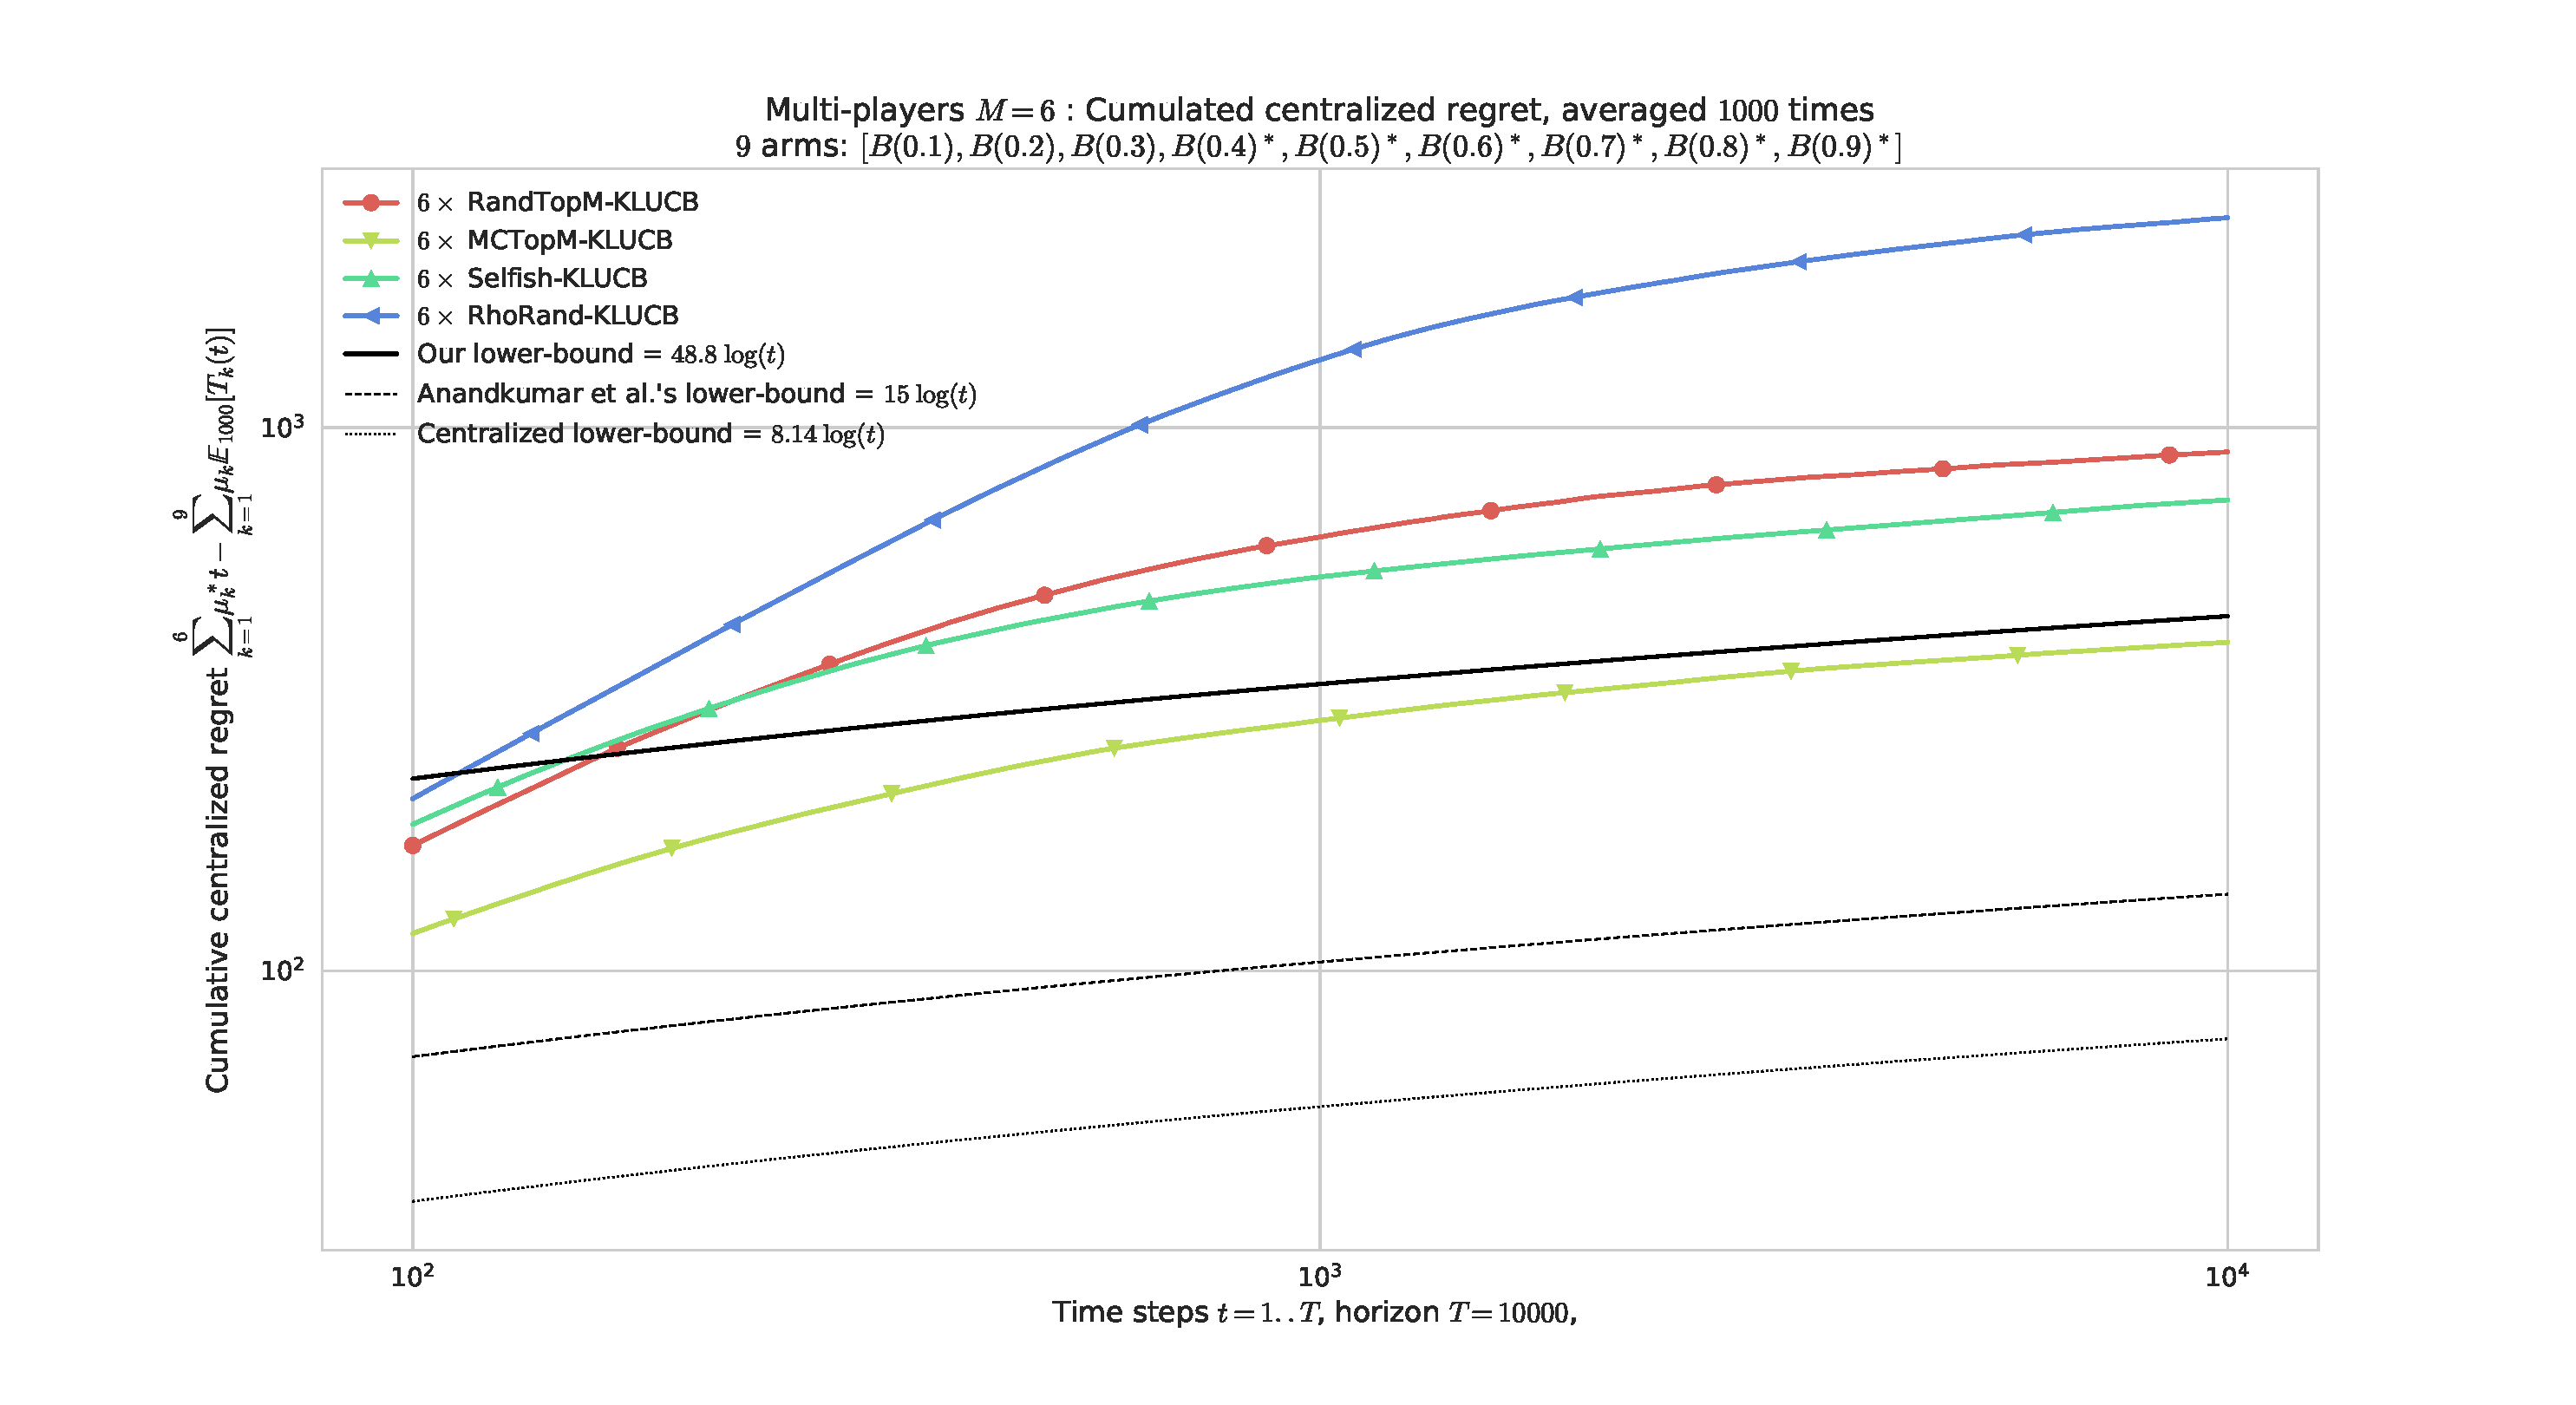
\includegraphics[width=1.00\textwidth]{MP__K9_M6_T10000_N1000__4_algos/all_RegretCentralized_loglog____env1-1_8200873569864822246.pdf}
  % \end{subfigure}
  % ~
  % \begin{subfigure}[!h]{1.00\textwidth}
      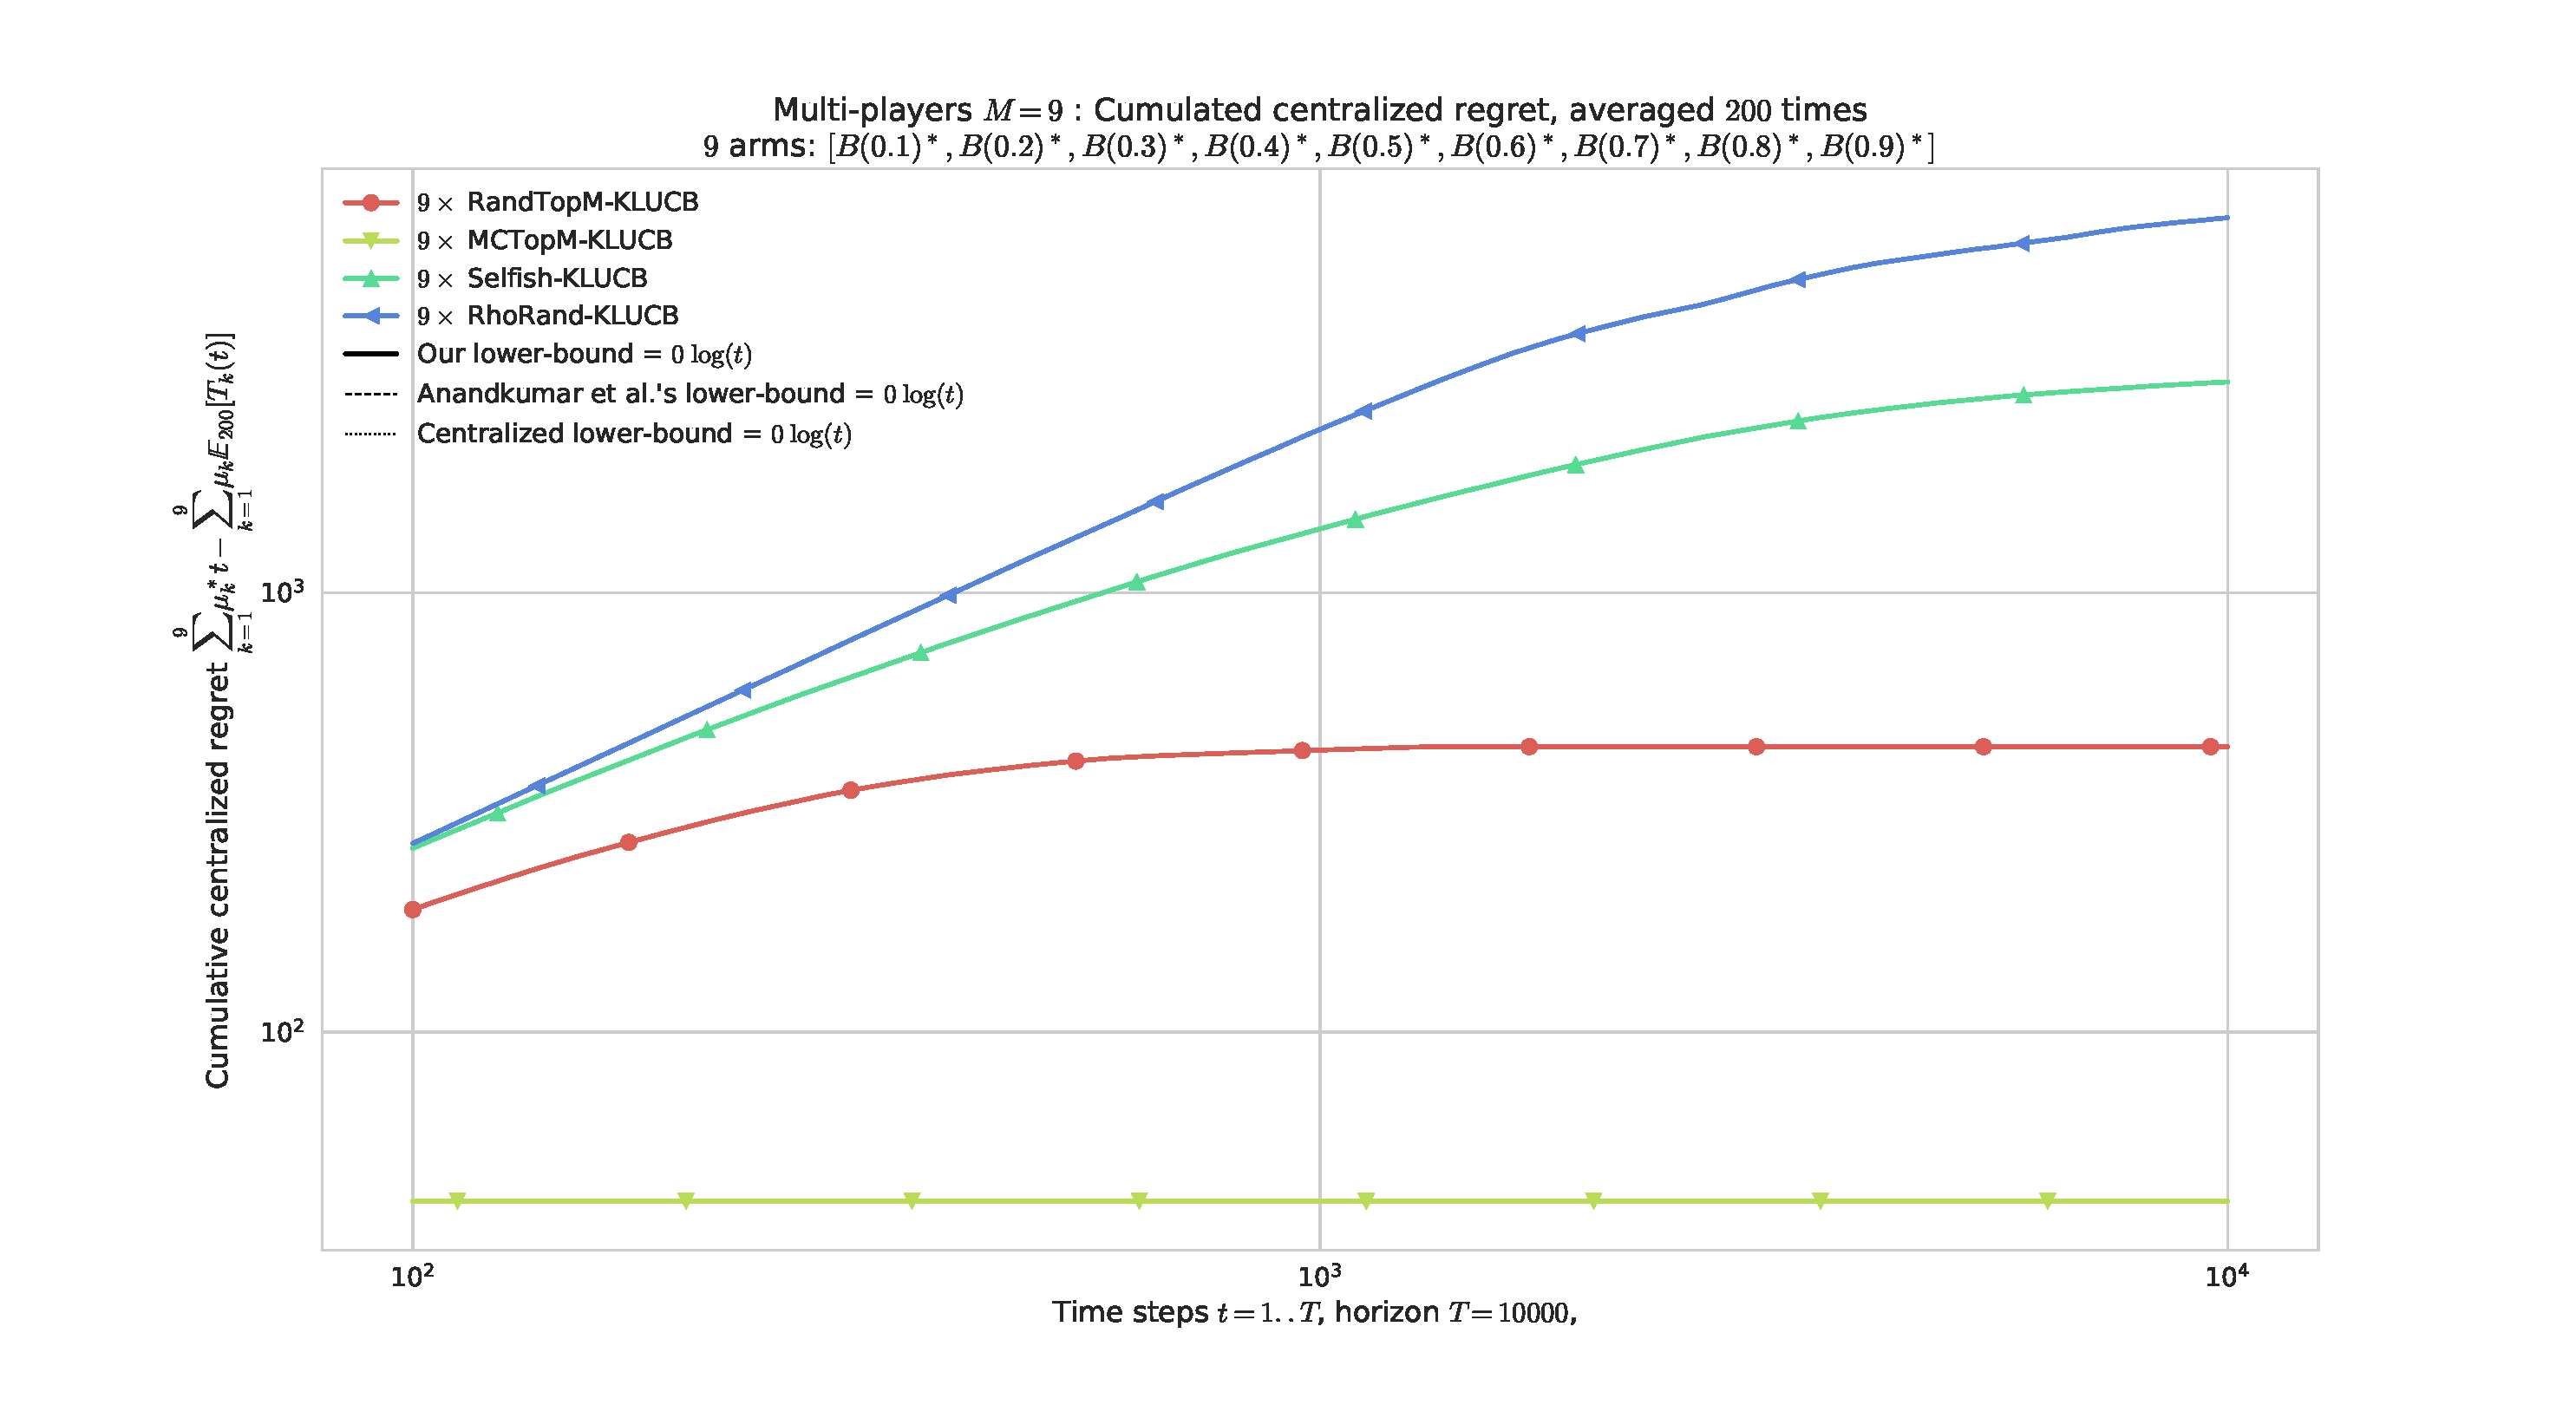
\includegraphics[width=1.10\textwidth]{MP__K9_M9_T10000_N200__4_algos/all_RegretCentralized_loglog____env1-1_2306423191427933958.pdf}
  % \end{subfigure}
  \caption[Regret for $M=2$ and $9$ players for $K=9$ arms, horizon $T=5000$, for a fixed problem.]{Regret (in log-log scale), for $M=2$ and $9$ players for $K=9$ arms, horizon $T=5000$, for problem $\boldsymbol{\mu}=[0.1,\dots,0.9]$] for problem $\boldsymbol{\mu}=[0.1,\dots,0.9]$. In different settings, \textcolor{lightgreen}{\RandTopM{} (in light green)} and \textcolor{darkgreen}{\Selfish{} (in green)} can outperform each other, and always outperform \rhoRand. \MCTopM{} is always among the best algorithms, and for $M$ not too small, its regret seems logarithmic with a constant matching the lower bound.}
  \label{fig:5:MP__K9_M2-6-9_T10000_N200__4_algos}
\end{figure}


% \begin{figure}[!t]
%   \centering
%   % \begin{subfigure}[!h]{0.75\textwidth}
%       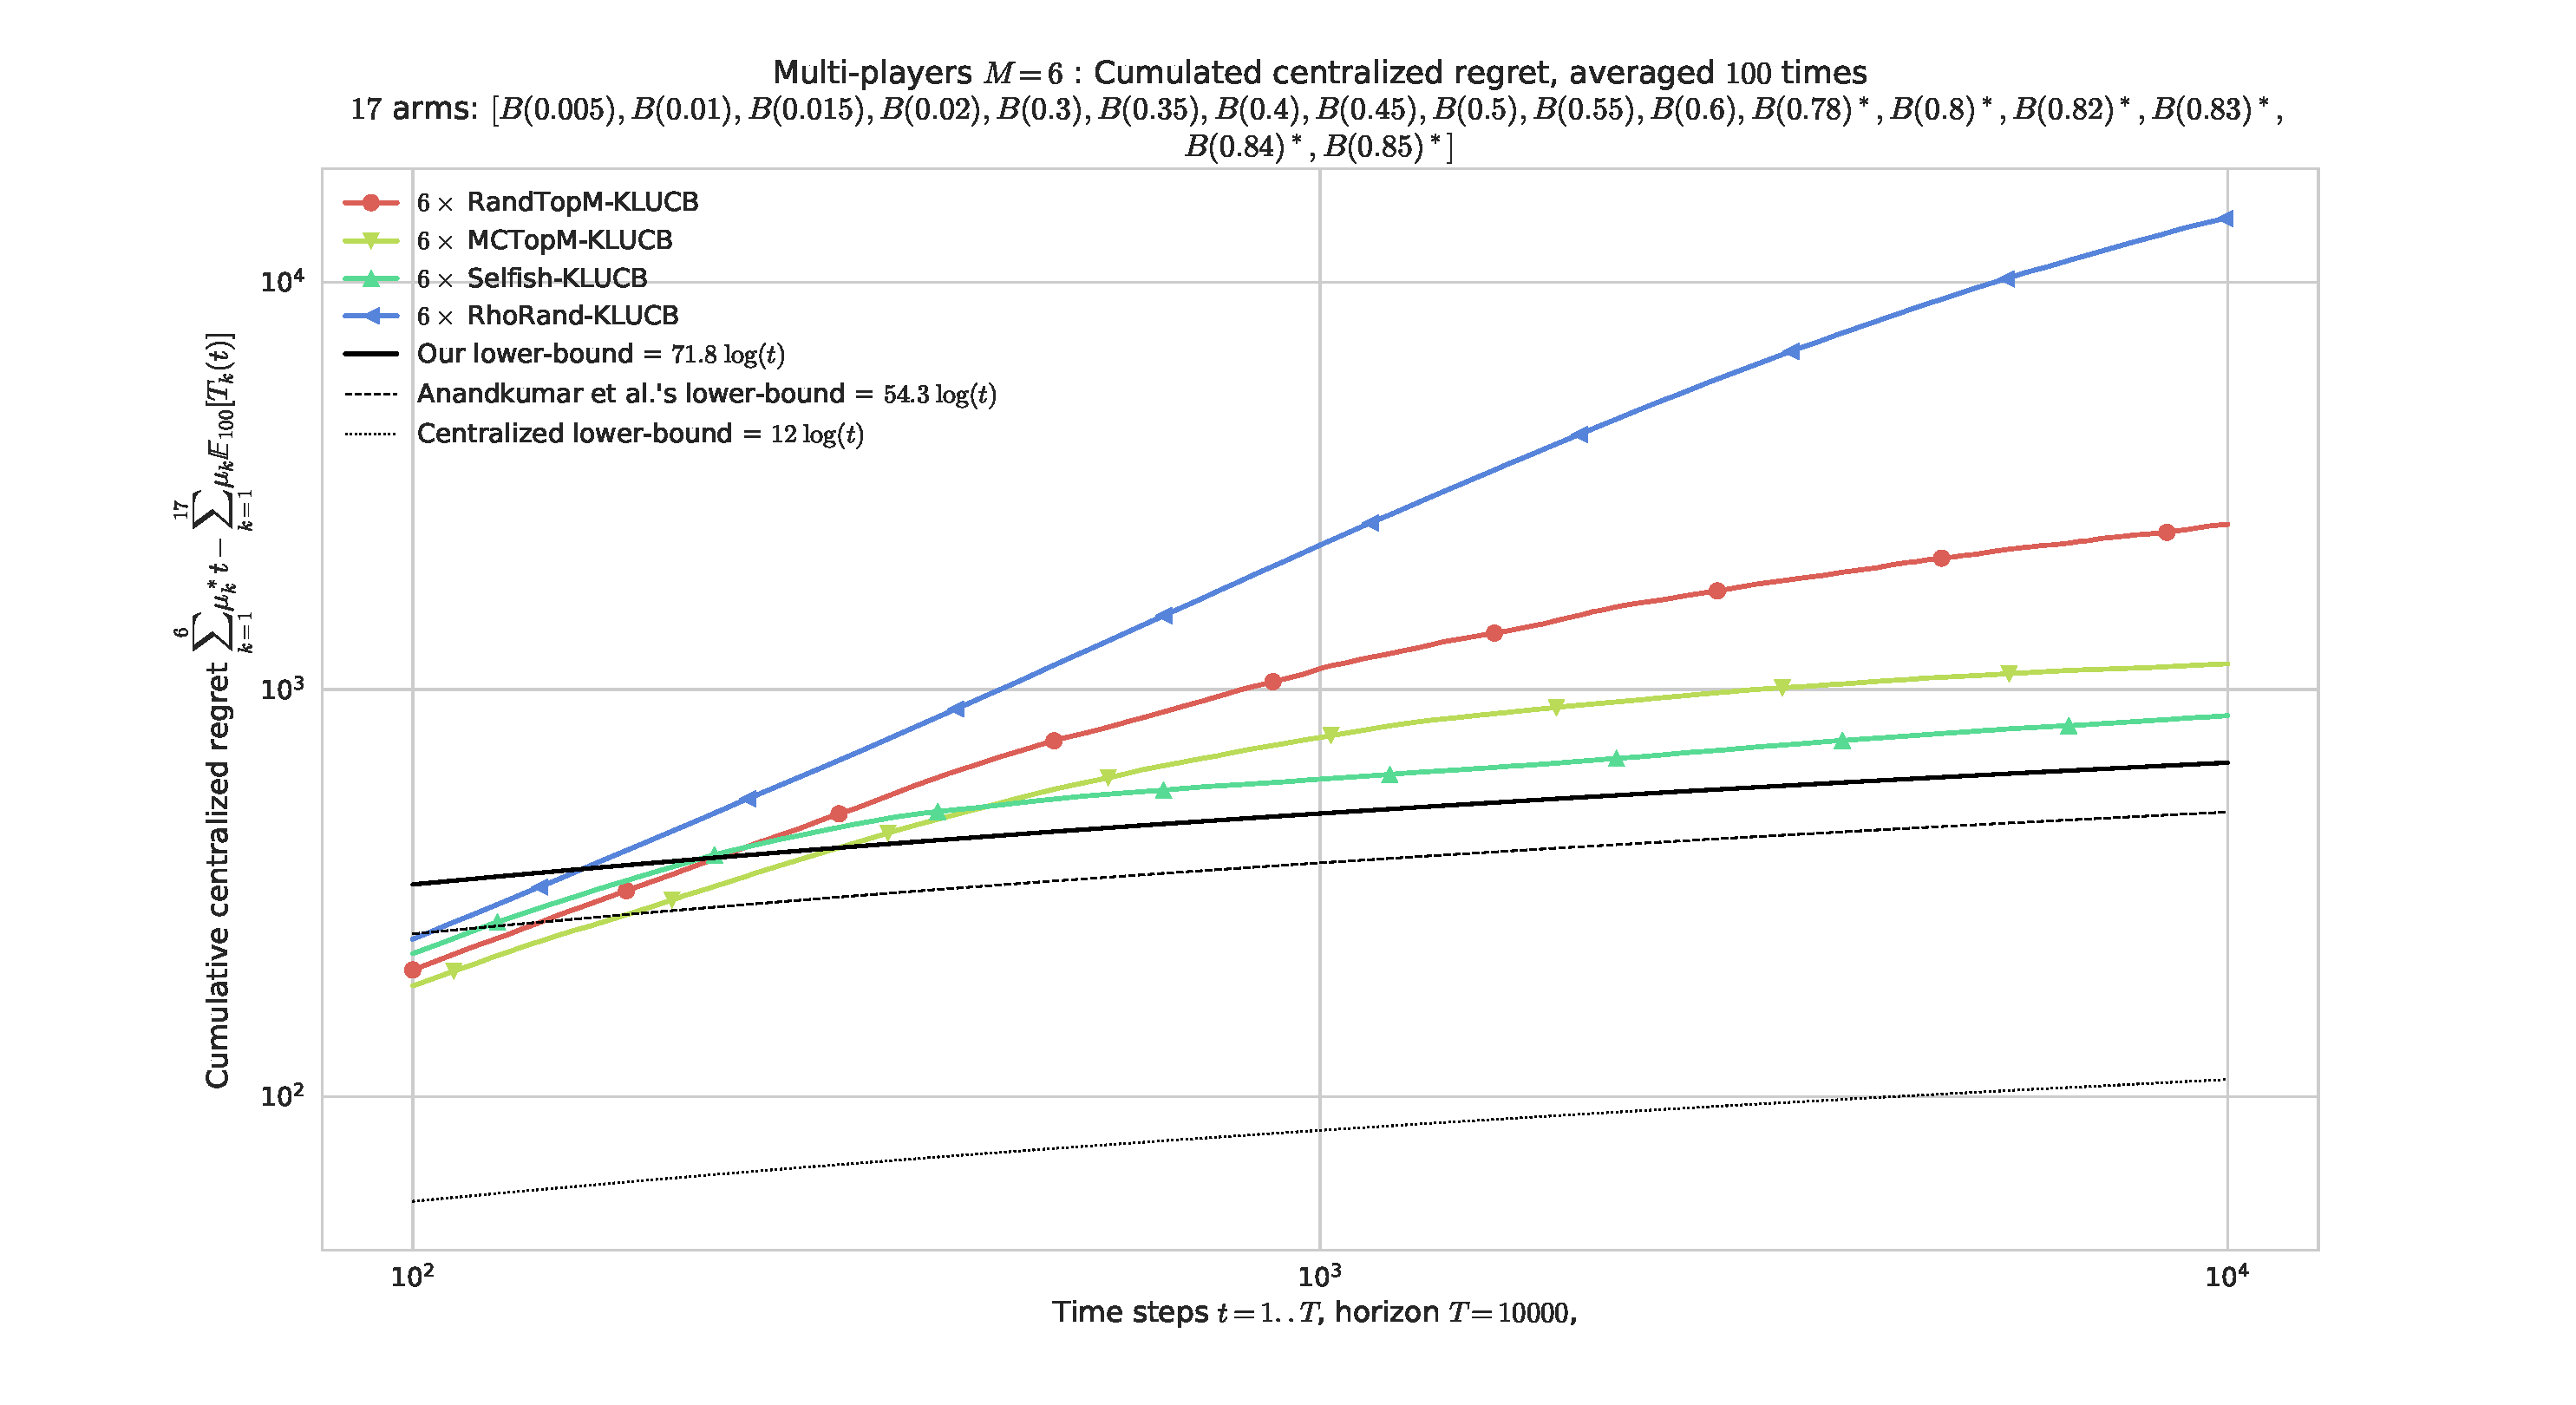
\includegraphics[width=0.75\textwidth]{MP__K17_M6_T10000_N100__4_algos/all_RegretCentralized_loglog____env1-1_4163066365888233475.pdf}
%   % \end{subfigure}
%   % ~
%   % \begin{subfigure}[!h]{0.75\textwidth}
%       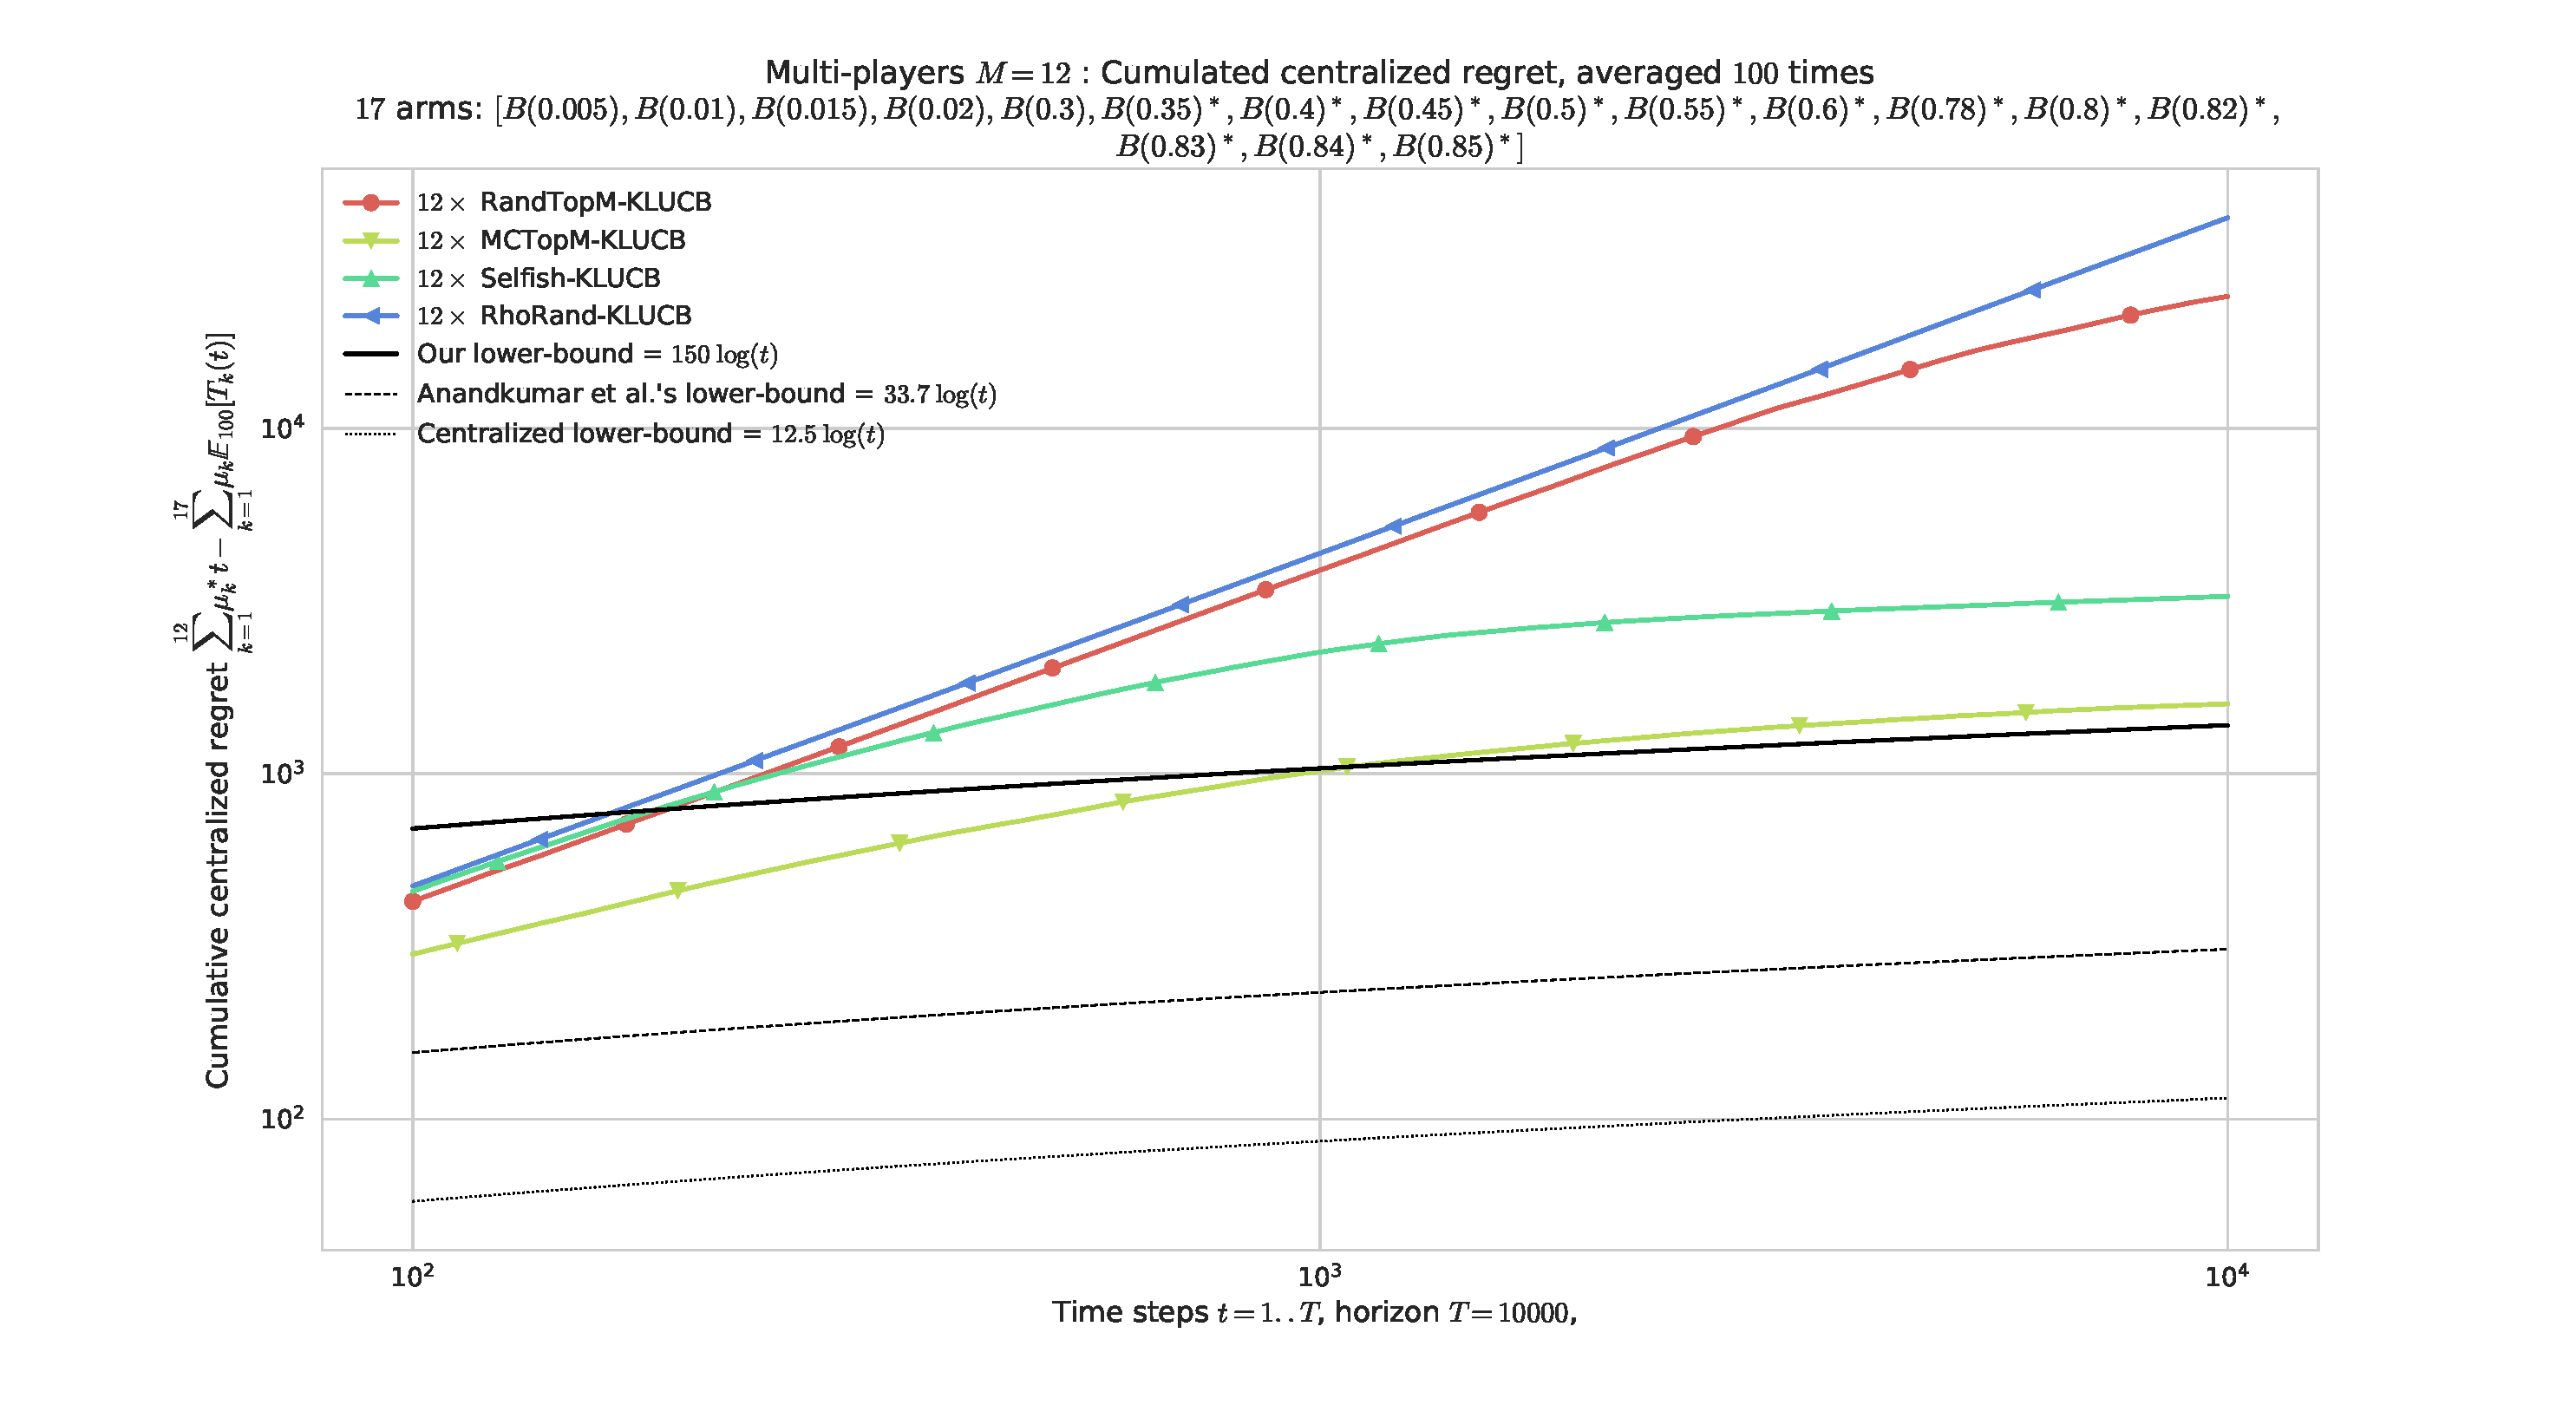
\includegraphics[width=0.75\textwidth]{MP__K17_M12_T10000_N100__4_algos/all_RegretCentralized_loglog____env1-1_3856003705095179548.pdf}
%   % \end{subfigure}
%   % ~
%   % \begin{subfigure}[!h]{0.75\textwidth}
%       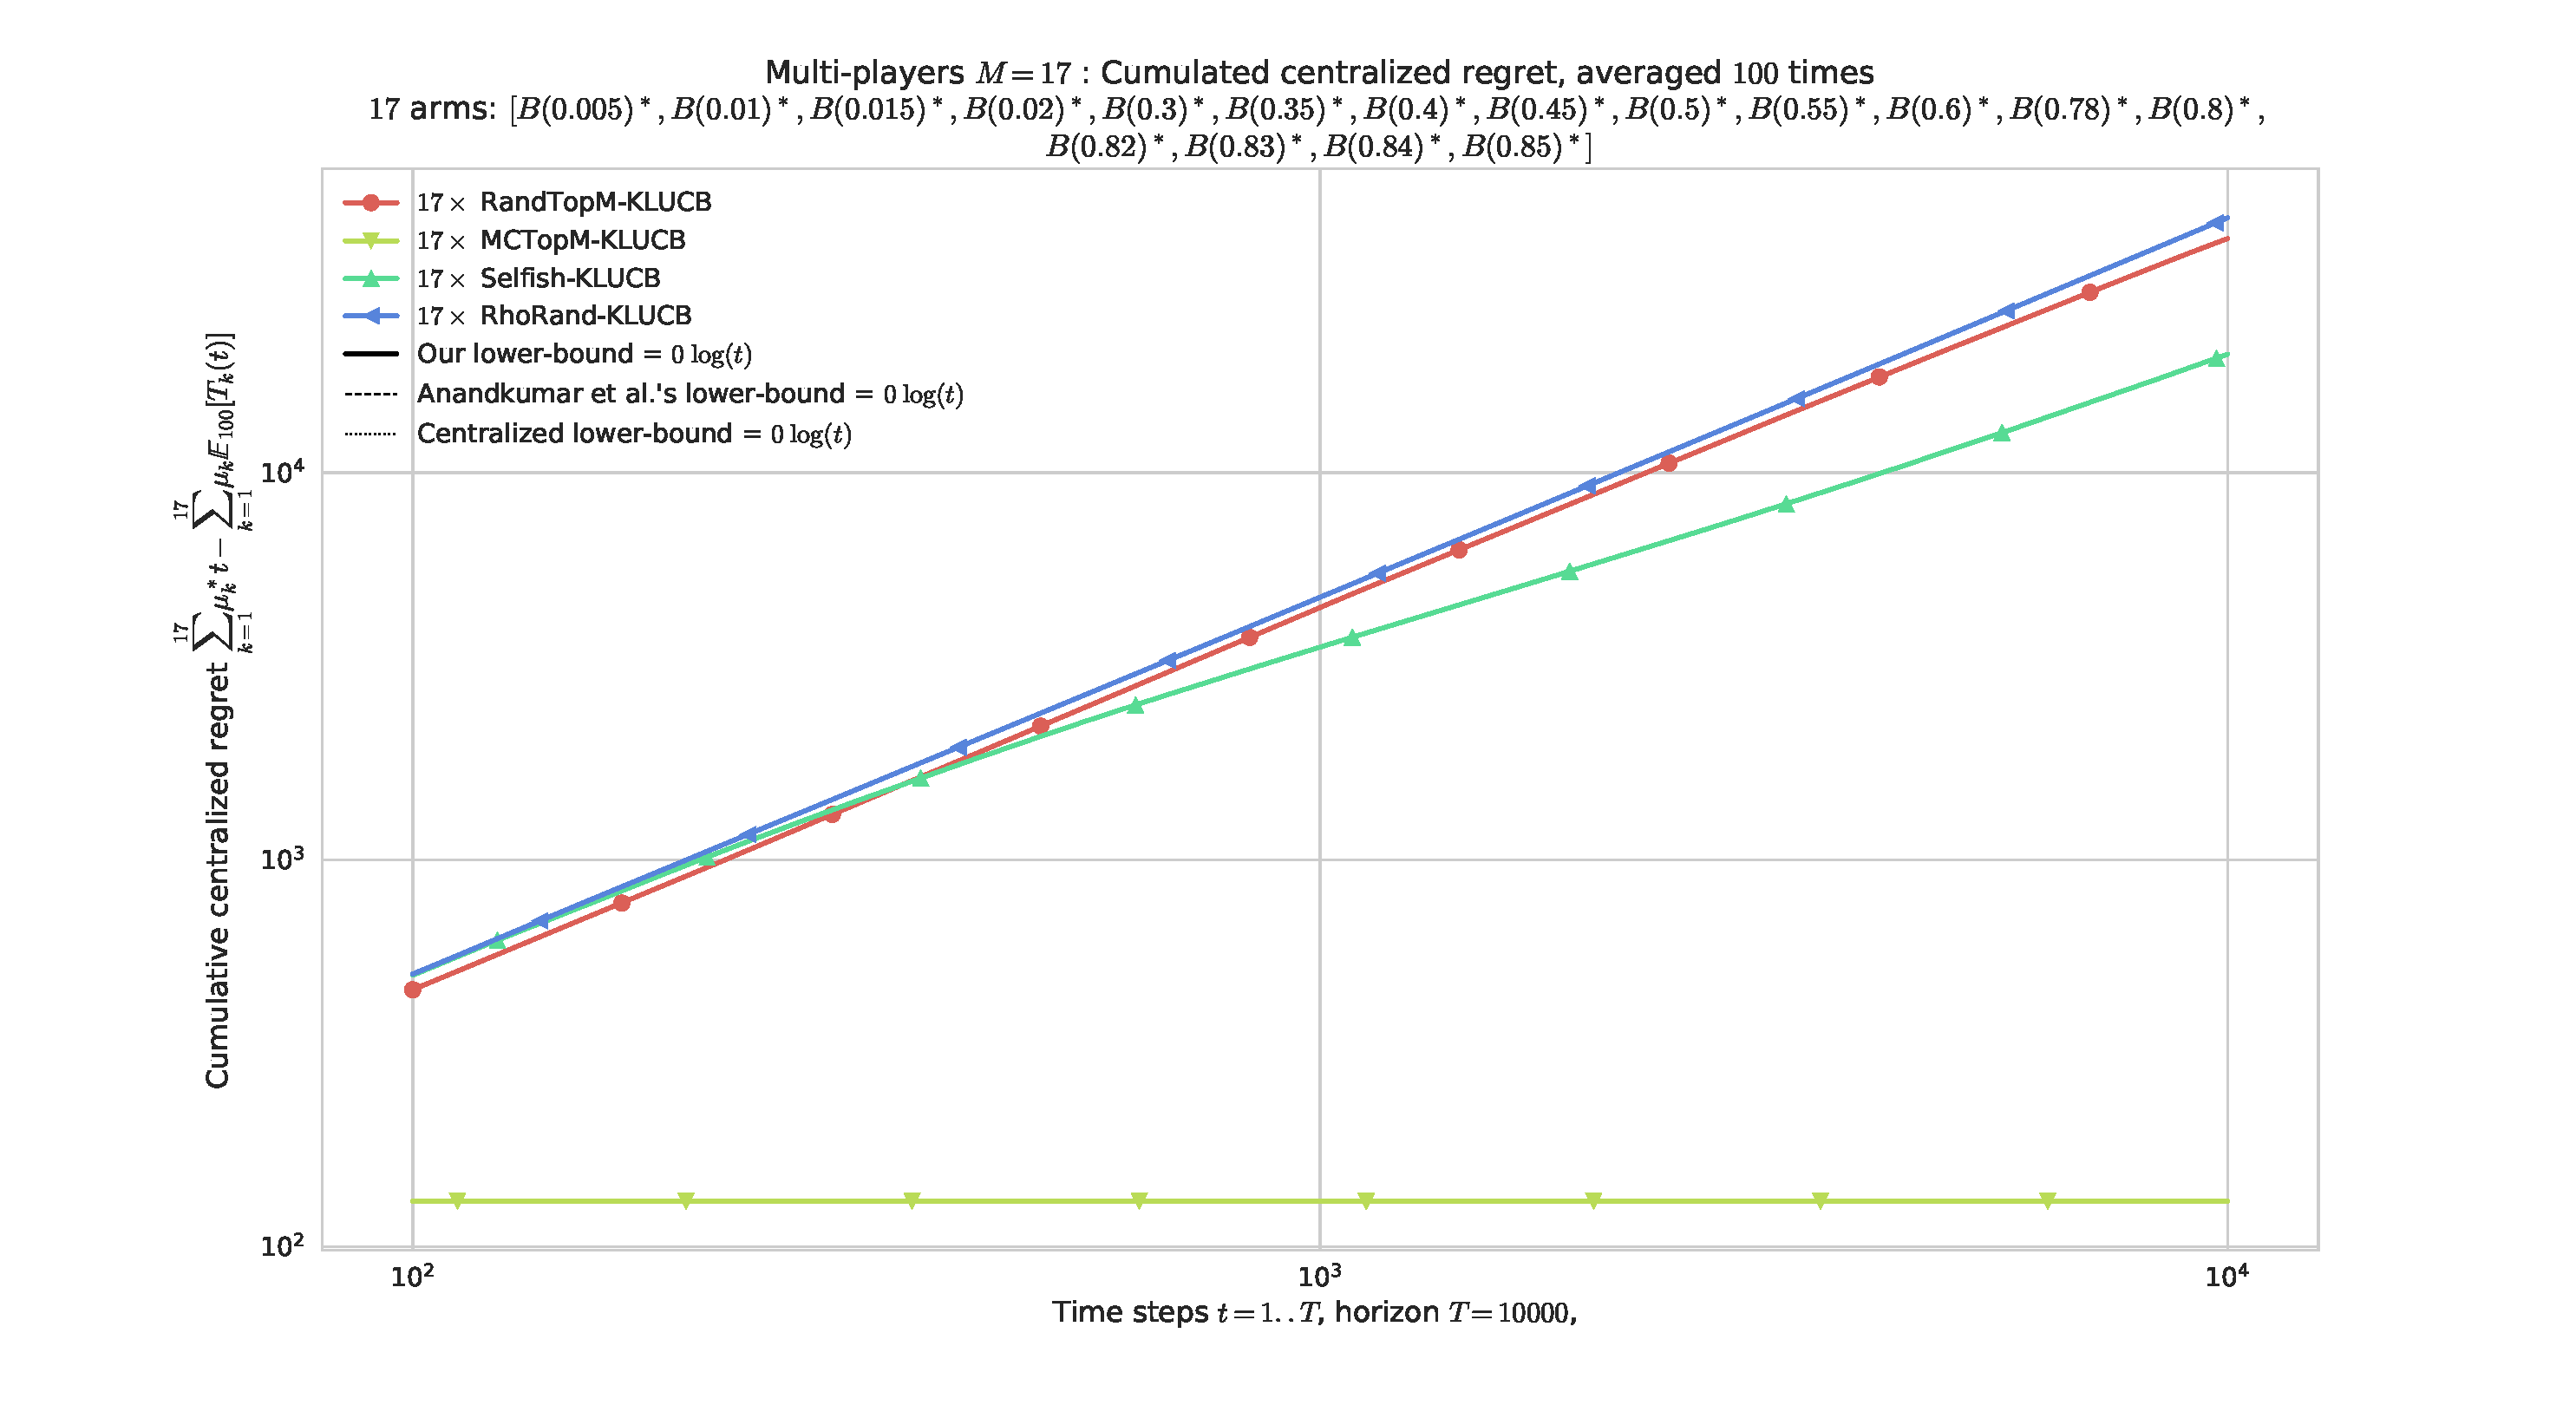
\includegraphics[width=0.75\textwidth]{MP__K17_M17_T10000_N100__4_algos/all_RegretCentralized_loglog____env1-1_8969236287861113966.pdf}
%   % \end{subfigure}
%   \caption[Regret for $M=6, 12, 17$ players for a ``difficult'' problem with $K=17$, and $T=5000$]{Regret (in log-log scale), for $M=6, 12, 17$ players for a ``difficult'' problem with $K=17$, and $T=5000$. The same observation as in Figure~\ref{fig:5:MP__K9_M2-6-9_T10000_N200__4_algos} can be made. \Selfish{} outperforms \MCTopM{} for $M=2$ here. Additionally, \MCTopM{} is the only algorithm to not fail dramatically when $M=K$ here.}
%   \label{fig:5:MP__K17_M6-12-17_T10000_N100__4_algos}
% \end{figure}




\begin{figure}[!t]
  \centering
  % \begin{subfigure}[!h]{0.85\textwidth}
      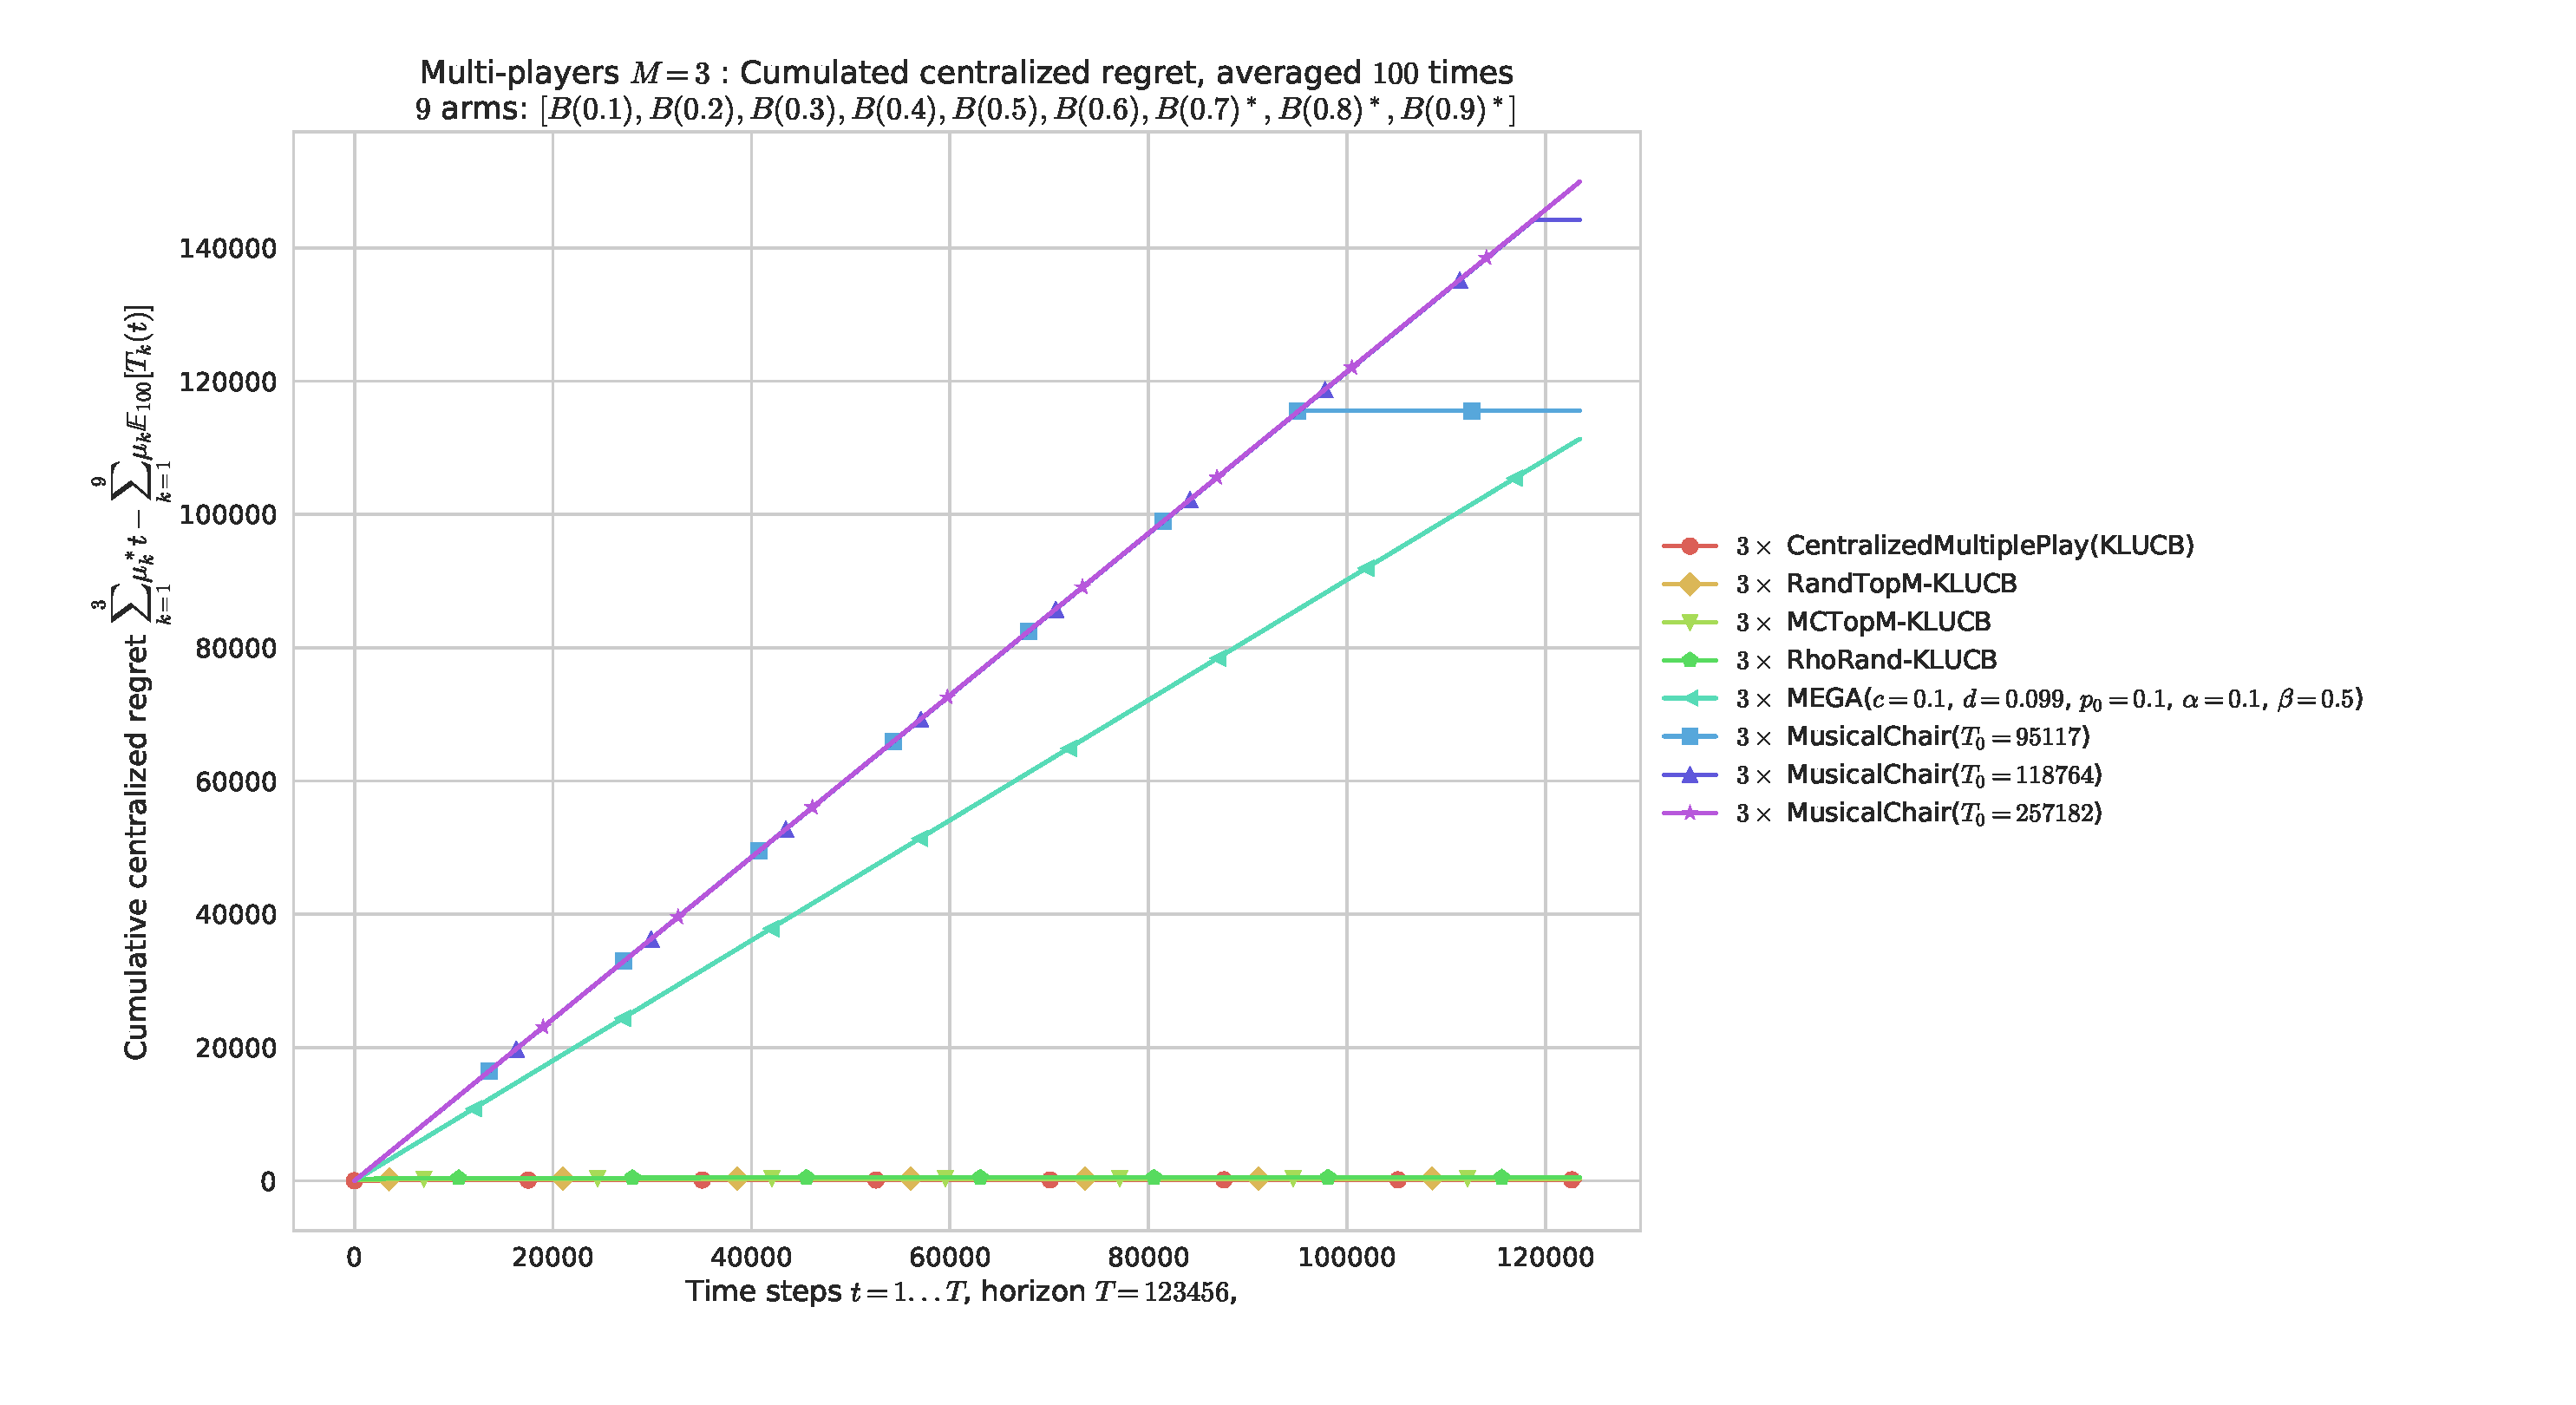
\includegraphics[width=1.00\textwidth]{MP__K9_M3_T123456_N100__8_algos/all_RegretCentralized____env1-1_7803645526012310577.pdf}
  % \end{subfigure}
  % ~
  % \begin{subfigure}[!h]{0.85\textwidth}
      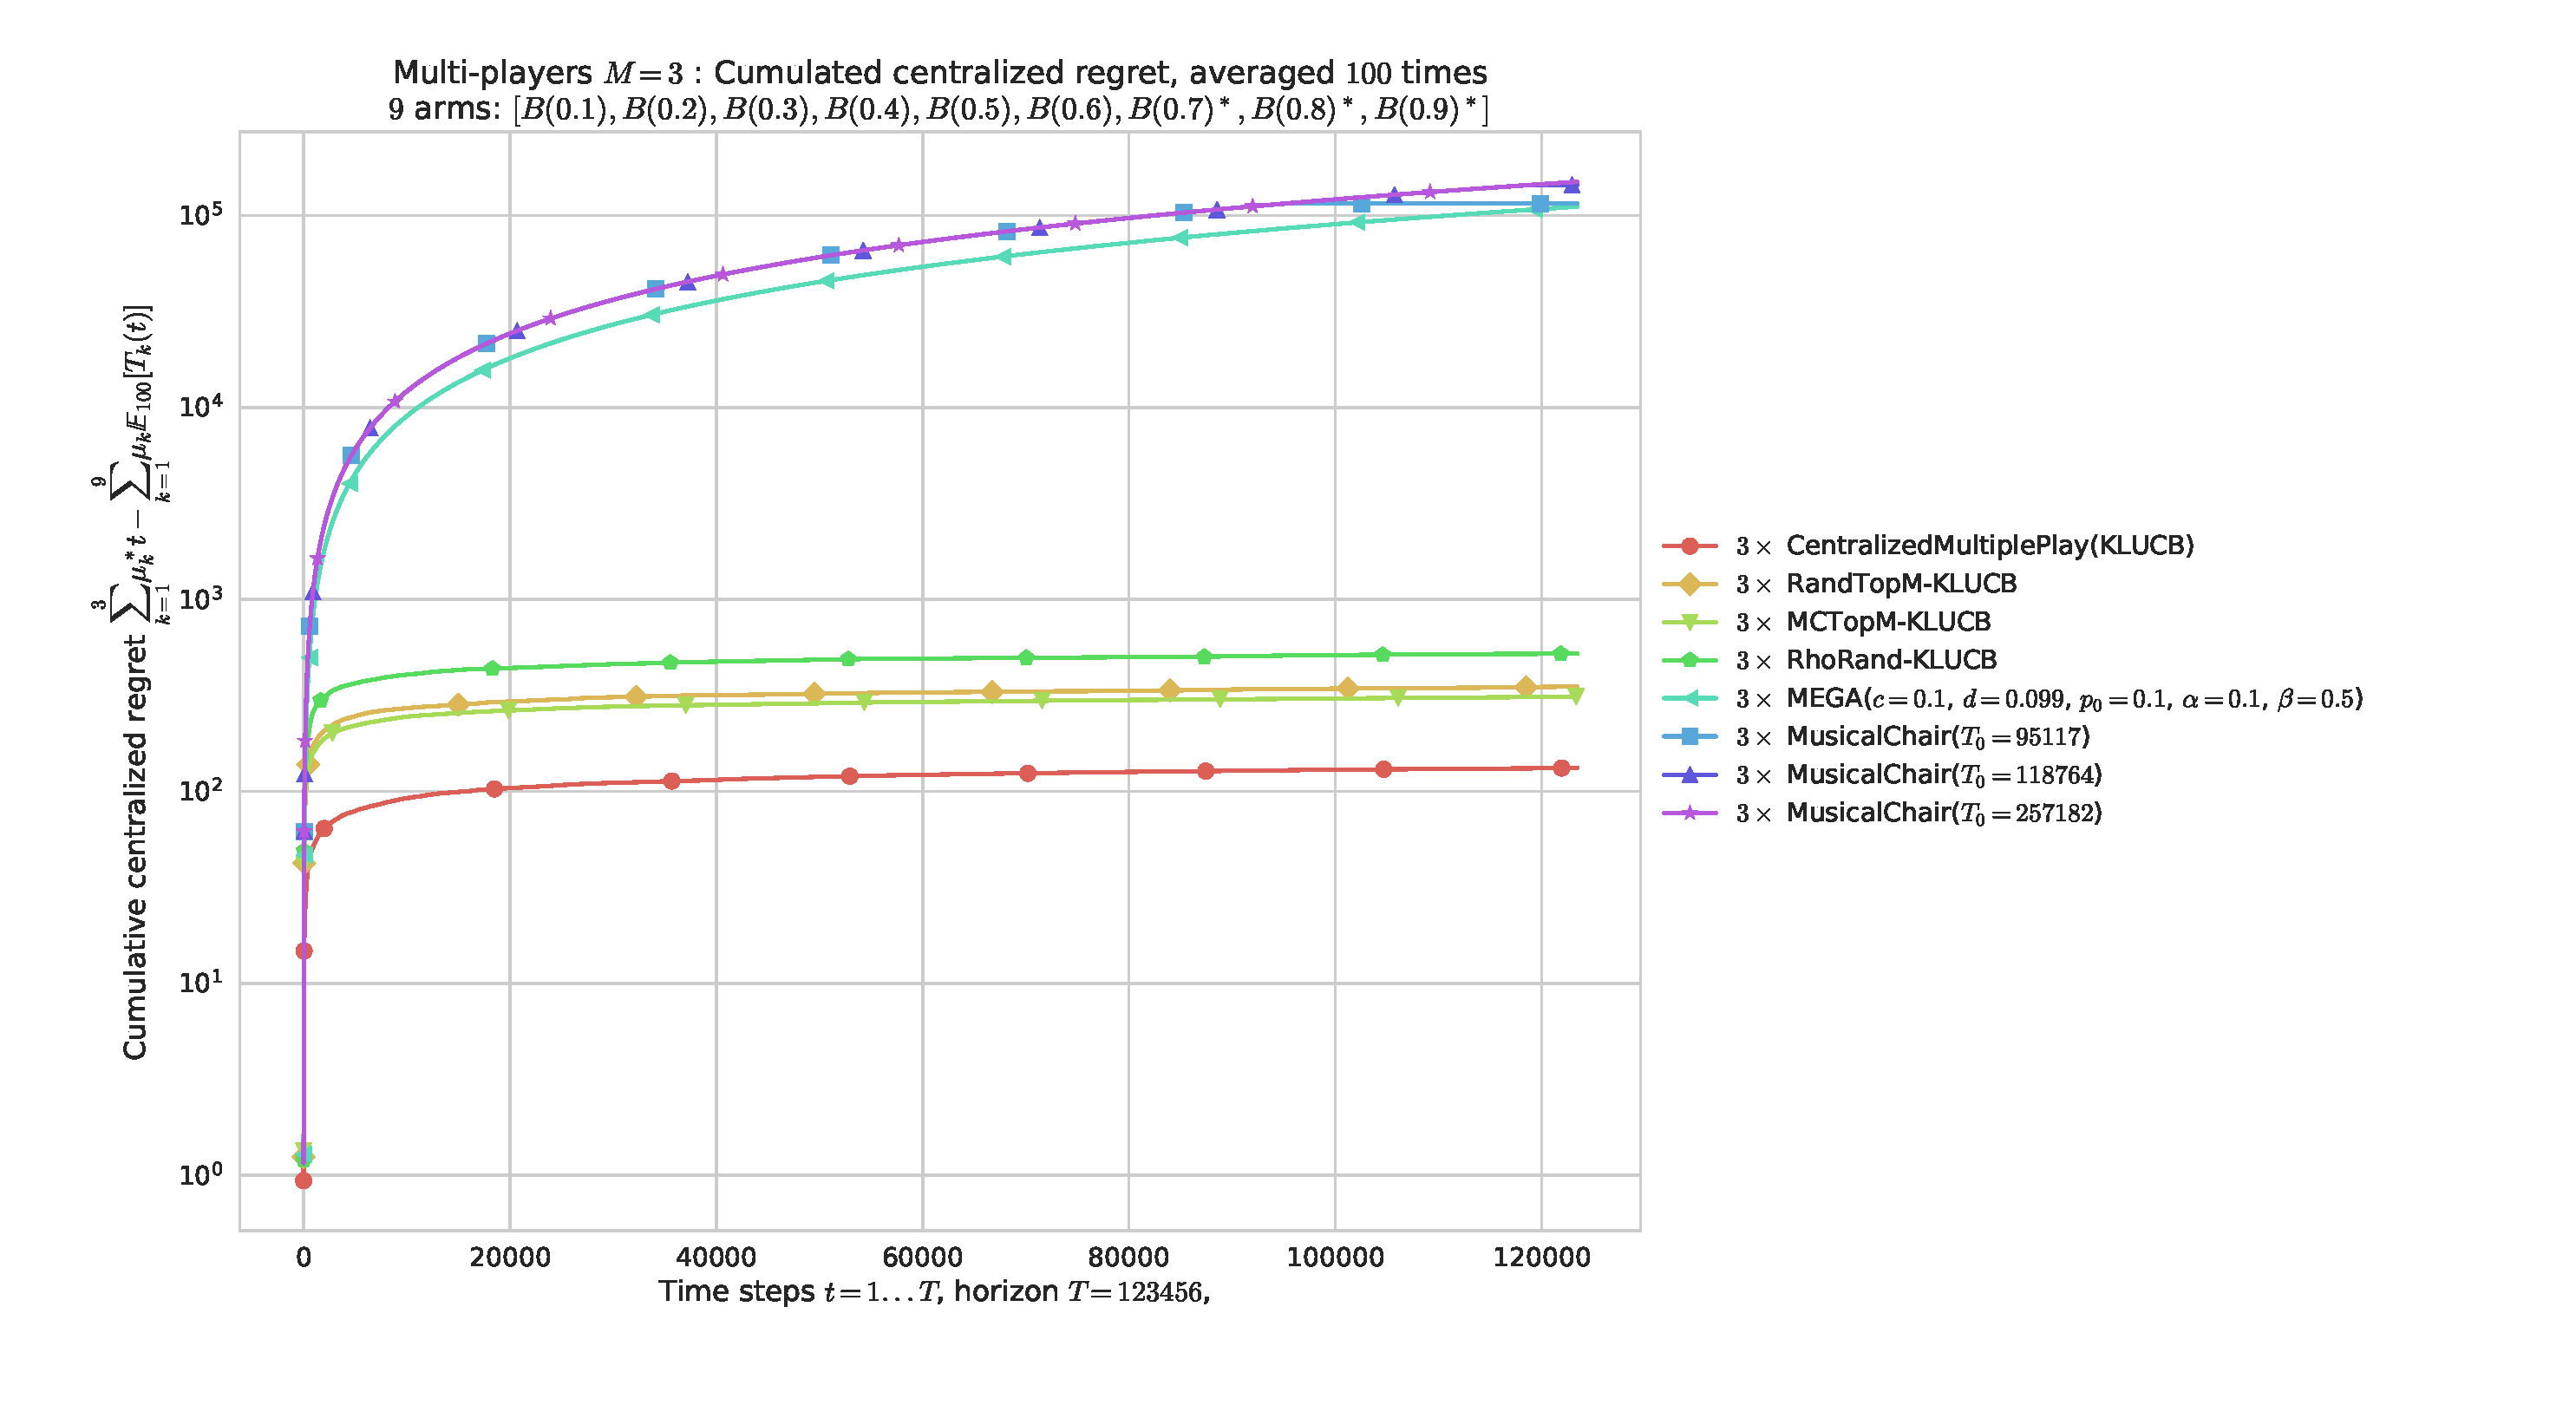
\includegraphics[width=1.00\textwidth]{MP__K9_M3_T123456_N100__8_algos/all_RegretCentralized_semilogy____env1-1_7803645526012310577.pdf}
  % \end{subfigure}
  \caption[Regret for $M=3$ players for $K=9$ arms, horizon $T=123456$, for $100$ repetitions on a fixed problem.]{Regret for $M=3$ players for $K=9$ arms, horizon $T=123456$, for $100$ repetitions on problem $\mu=[0.1,\dots,0.9]$. With a perfect knowledge on the horizon and the gap ($\Delta=0.1$ here) and by using the parameters suggested from their respective articles, \MEGA{} and \MusicalChair{} perform badly, even in this simple setting. The first two \MusicalChair{} instances use the optimal $T_0$ value from \cite{Rosenski16}, with $\varepsilon$ taken slightly smaller than the gap $\Delta$ ($\varepsilon=0.99 \Delta$), and respectively with $\delta=0.5$ and $\delta=0.1$, for which the regret can be bounded with probability $0.5$ and $0.9$ respectively. The third instance uses the optimal $T_0$ corresponding to $\delta=1/T$, that is guaranteed to have an expected regret of order $\log(T)$. The log-$y$ scale is used to easily differentiate between the different algorithms, and highlight that our proposal (in \textcolor{lightgreen}{light green $\nabla$}) outperform both \MEGA{} and \MusicalChair{} by three orders of magnitudes!}
  \label{fig:5:MP__K9_M3_T123456_N100__8_algos}
\end{figure}



%
% Regular plots of centralized regrets
%
\begin{figure}[!t]
  % \centering
  % \begin{subfigure}[!h]{0.49\textwidth}
  %   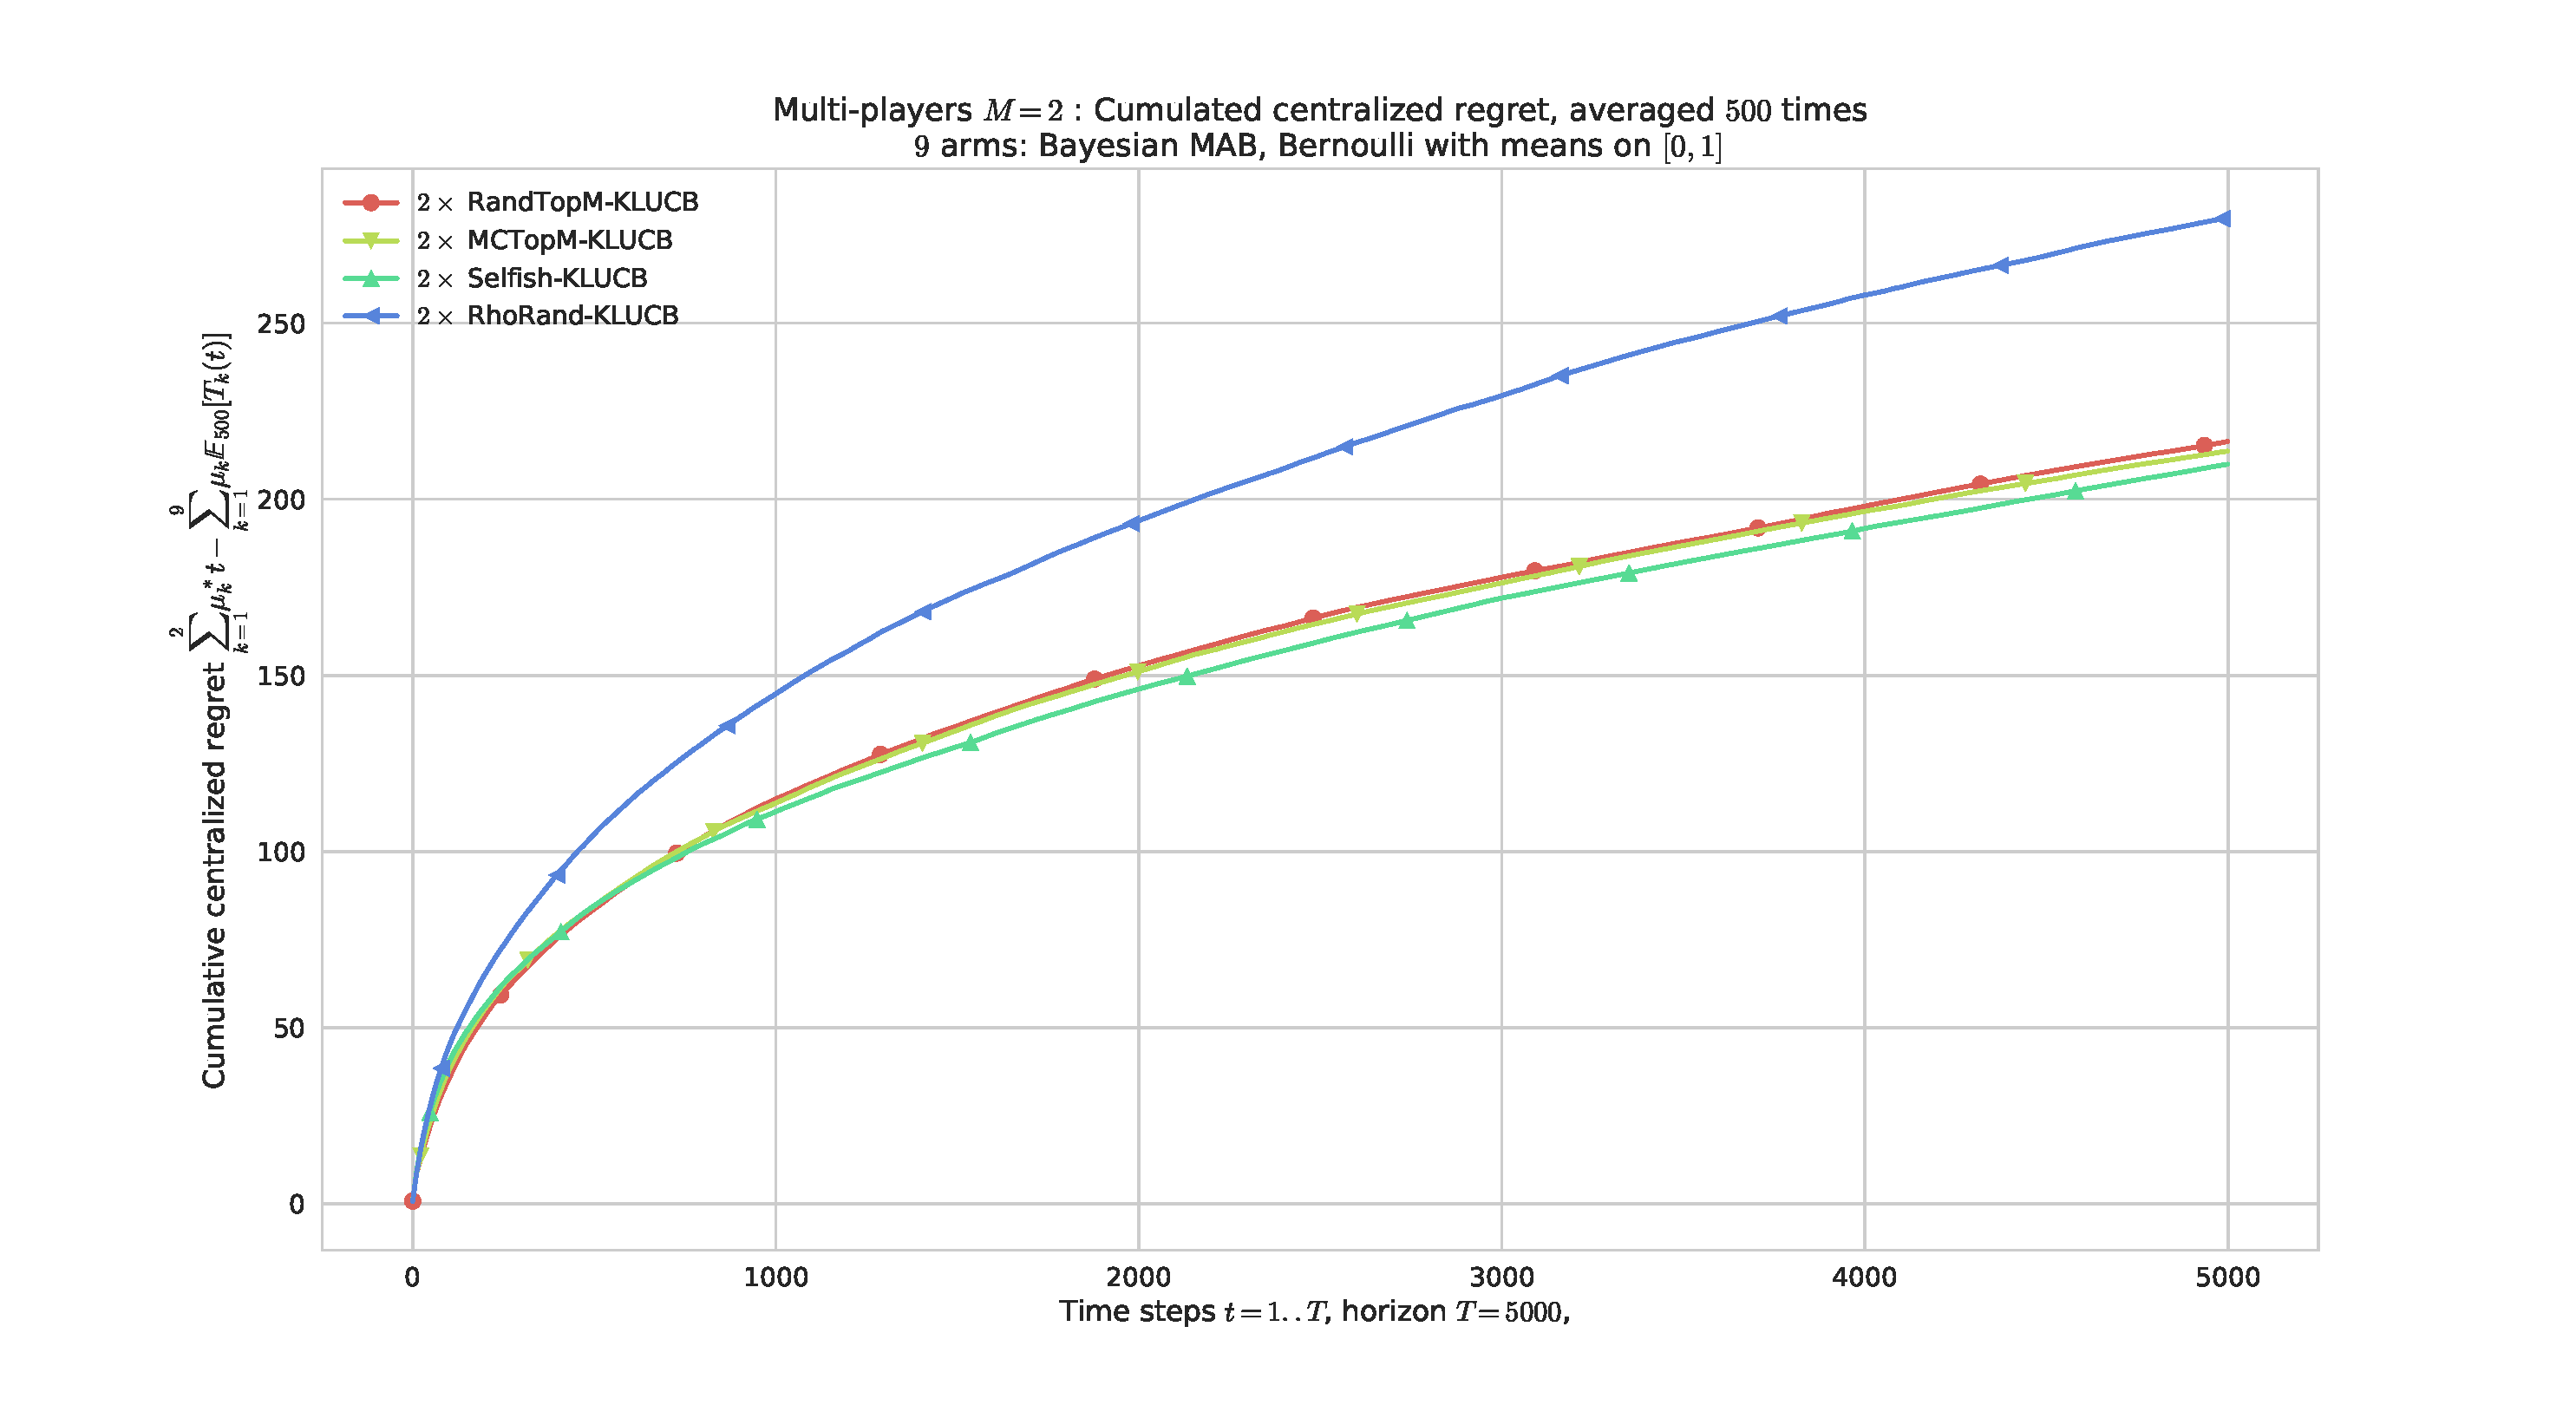
\includegraphics[width=1.00\textwidth]{MP__K9_M2_T5000_N500__4_algos/all_RegretCentralized____env1-1_3251433209347345969.pdf}
  % \end{subfigure}
  % % ~
  % \begin{subfigure}[!h]{0.49\textwidth}
    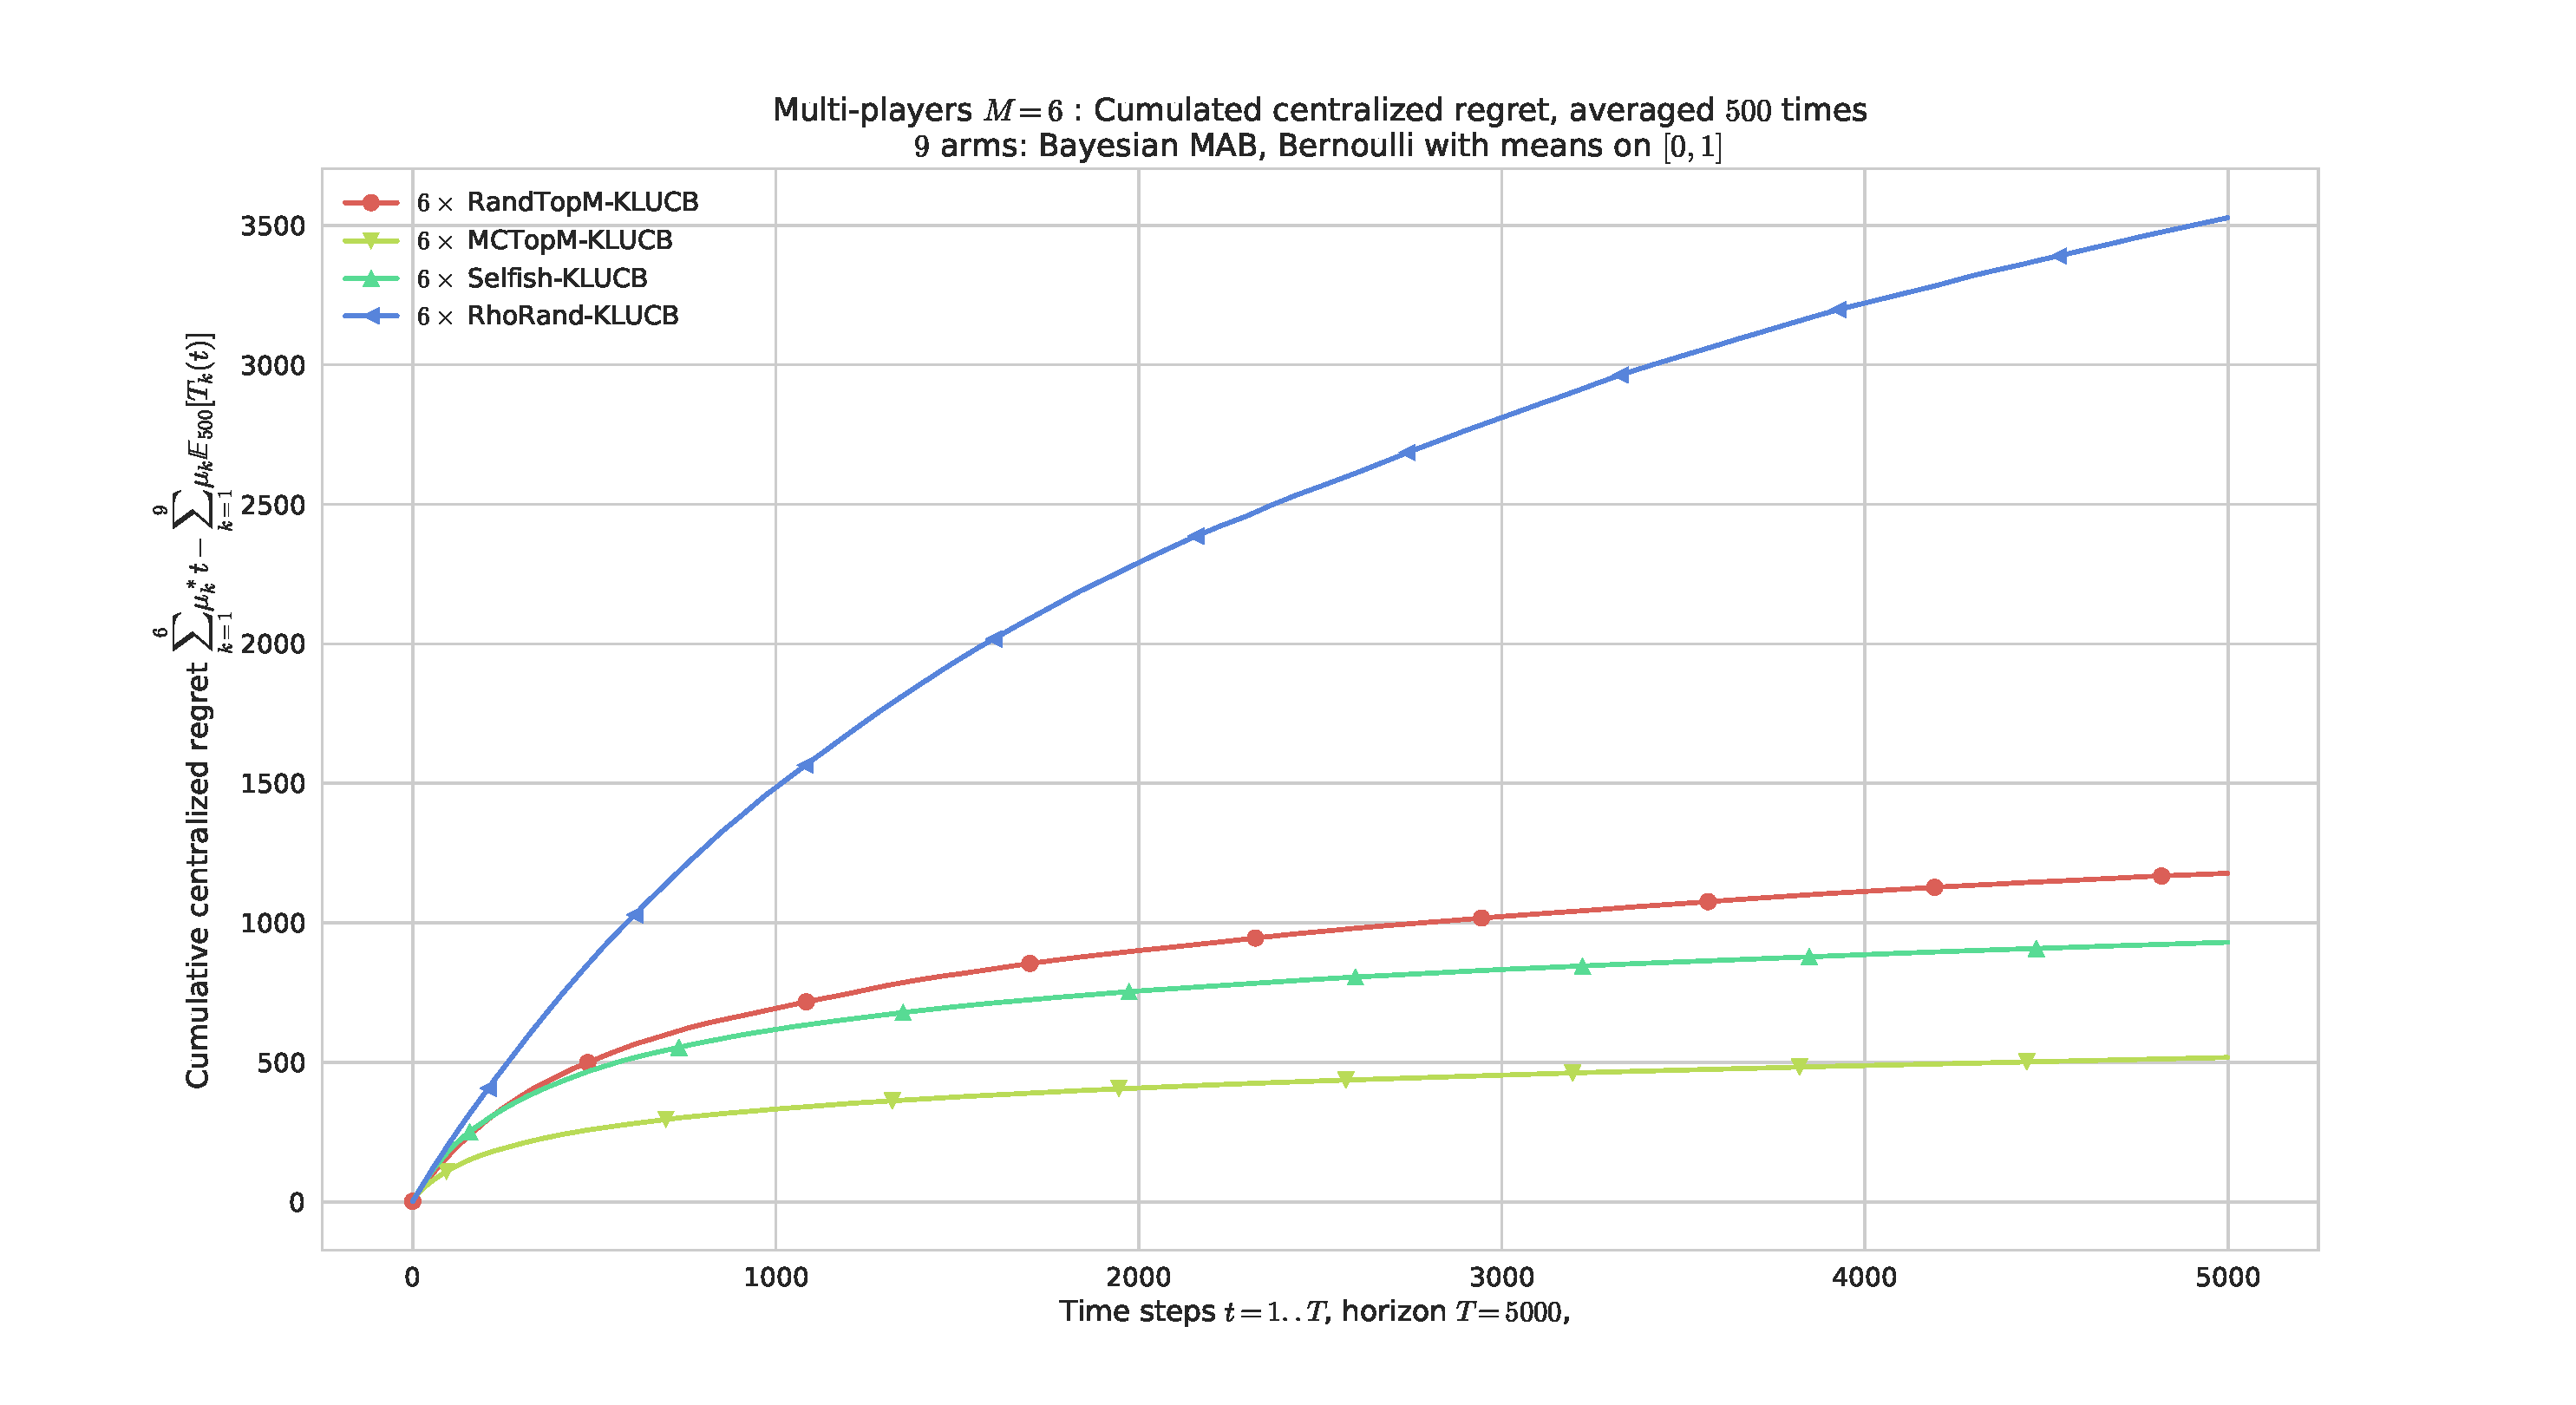
\includegraphics[width=1.05\textwidth]{MP__K9_M6_T5000_N500__4_algos/all_RegretCentralized____env1-1_8318947830261751207.pdf}
  % \end{subfigure}
  \caption[Regret for $M=6$ players, $K=9$ arms, horizon $T=5000$, against $500$ problems $\boldsymbol{\mu}$ uniformly sampled.]{Regret for $M=6$ players, $K=9$ arms, horizon $T=5000$, against $500$ problems $\boldsymbol{\mu}$ uniformly sampled in $[0,1]^K$. \textcolor{blue}{\rhoRand{} (top blue)} is outperformed by the other algorithms (and the gain increases with $M$). \textcolor{lightgreen}{\MCTopM{} (bottom green)} outperforms all the other algorithms in most cases.}
  % \label{fig:5:MP__K9_M2-6_T5000_N500__4_algos__all_RegretCentralized__BayesianProblems}
  \label{fig:5:MP__K9_M6_T5000_N500__4_algos__all_RegretCentralized__BayesianProblems}
  % \vspace*{-15pt}  % XXX remove if problem
\end{figure}


%
% Regular plots of centralized regrets
%
% \begin{figure}[!t]
%   \centering
%   % \begin{subfigure}[!h]{0.49\textwidth}
%       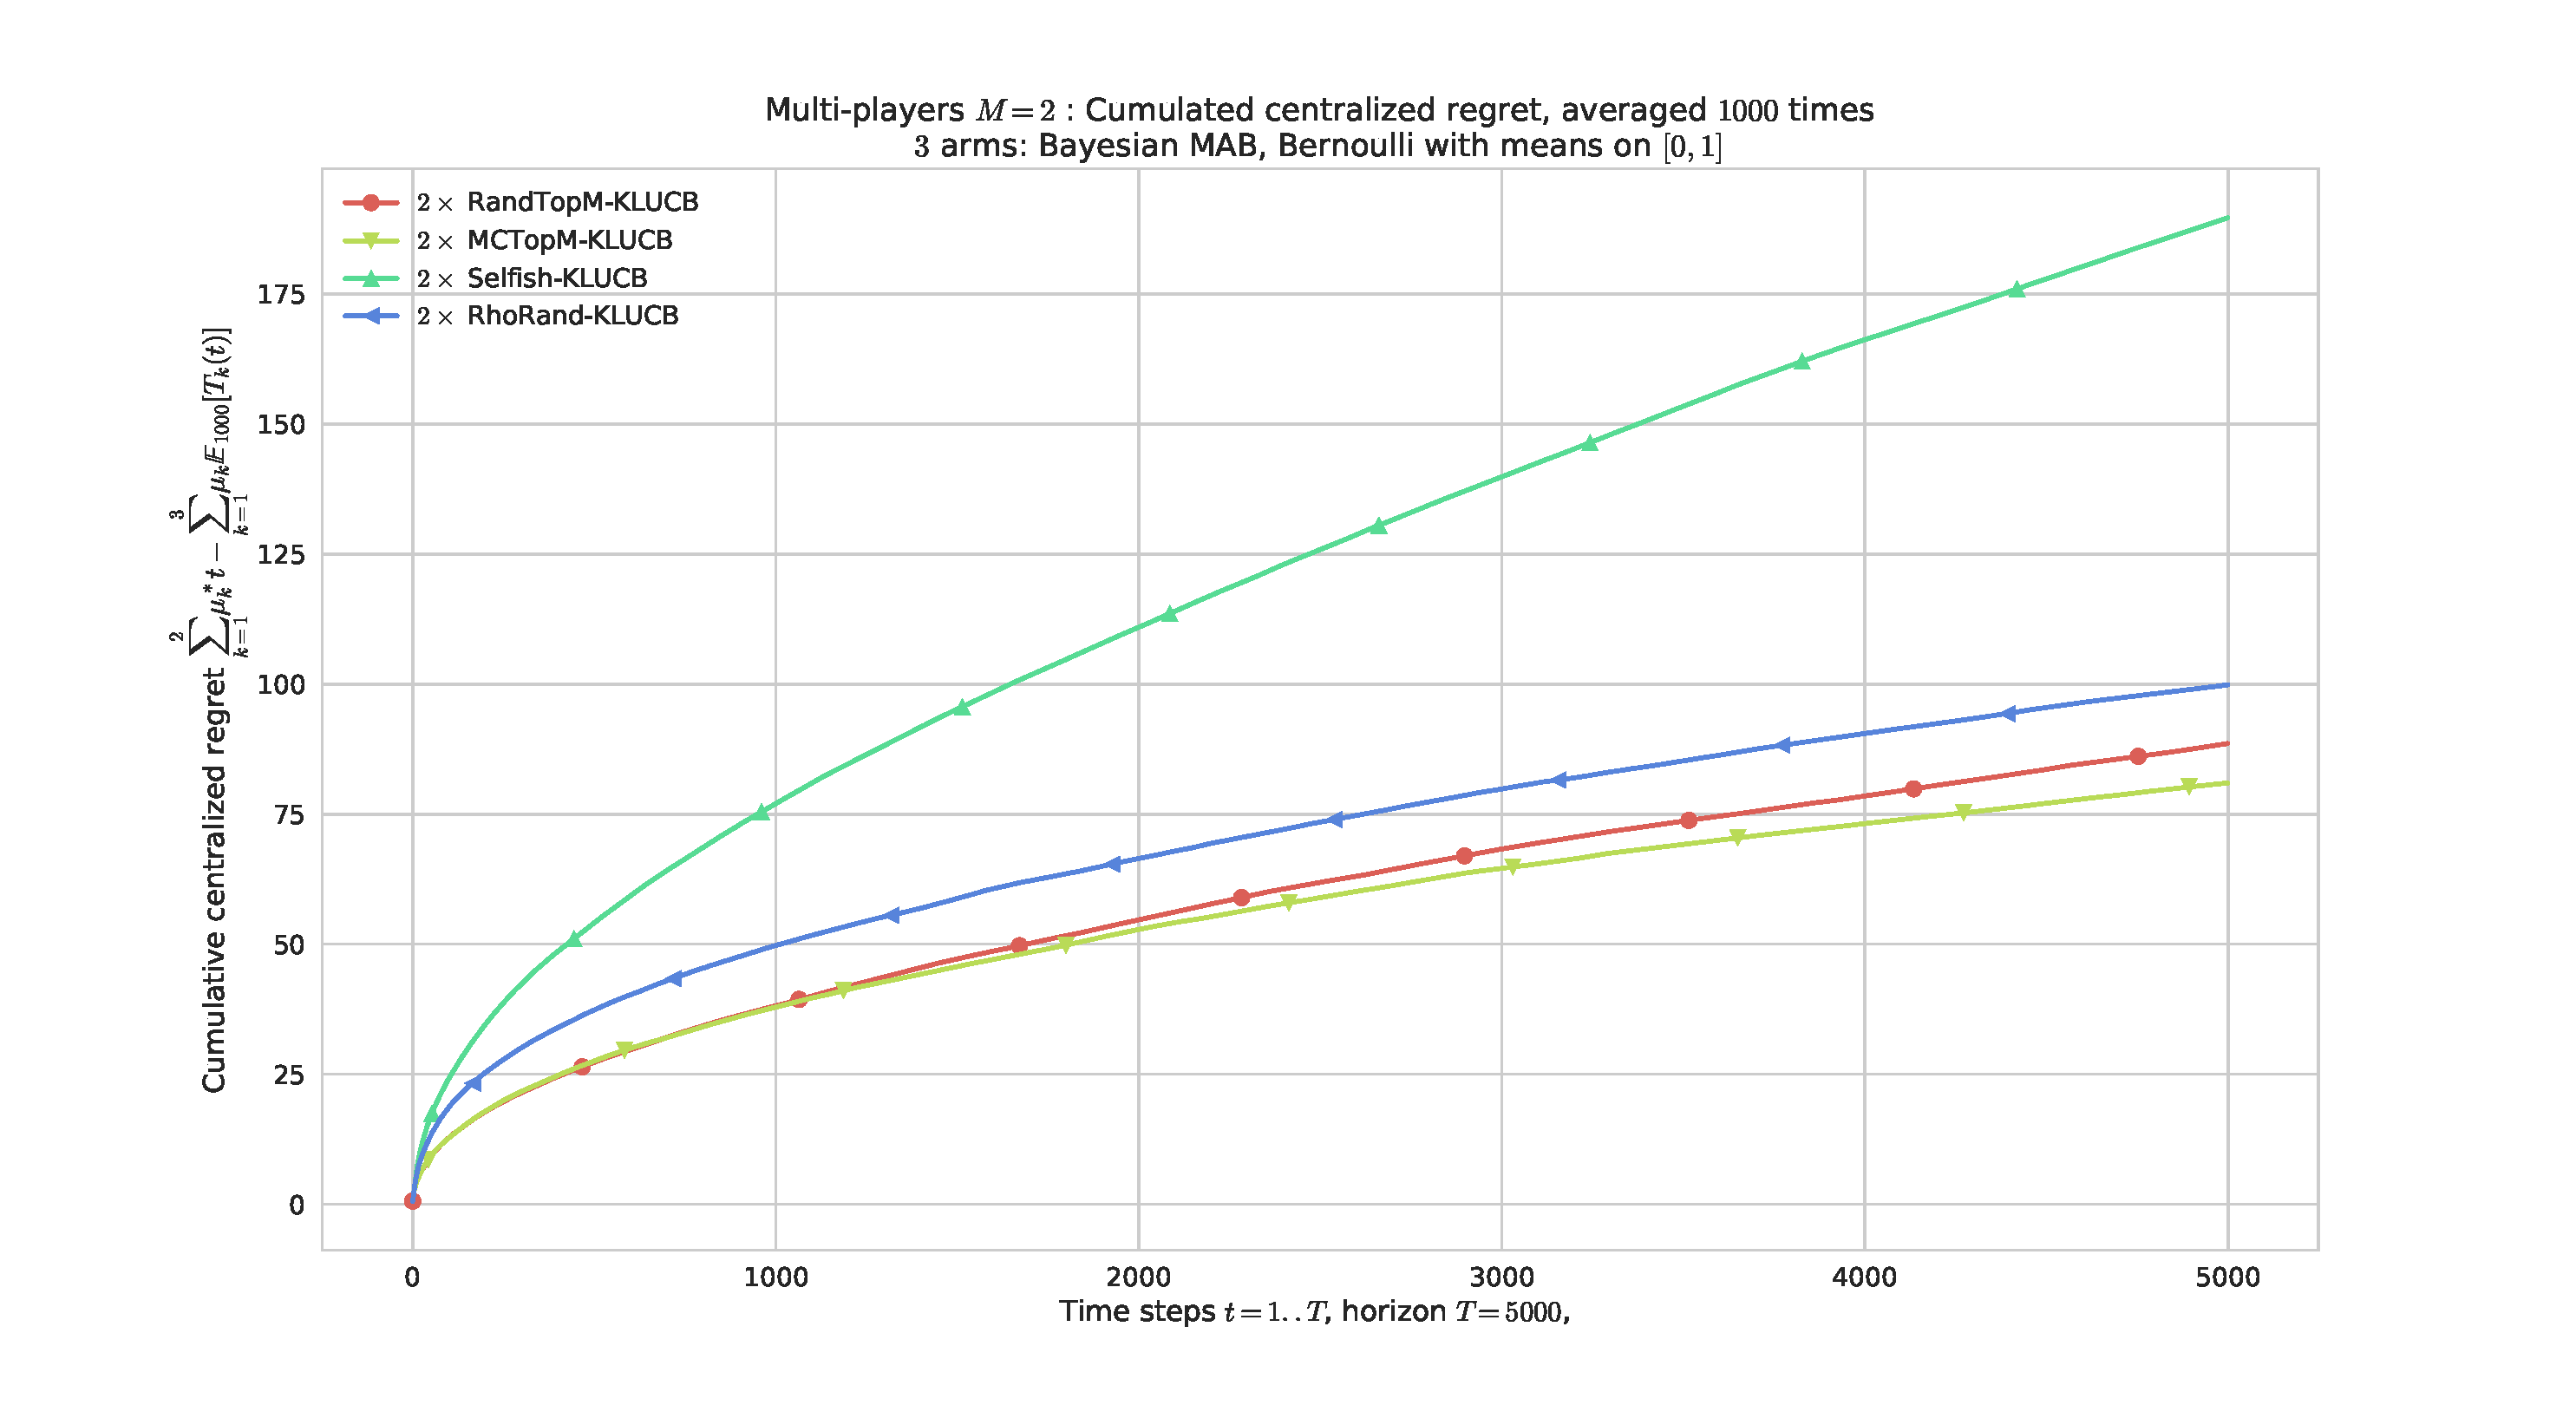
\includegraphics[width=1.05\textwidth]{MP__K3_M2_T5000_N1000__4_algos/all_RegretCentralized____env1-1_2643560344649862285.pdf}
%   % \end{subfigure}
%   % ~
%   % \begin{subfigure}[!h]{0.49\textwidth}
%       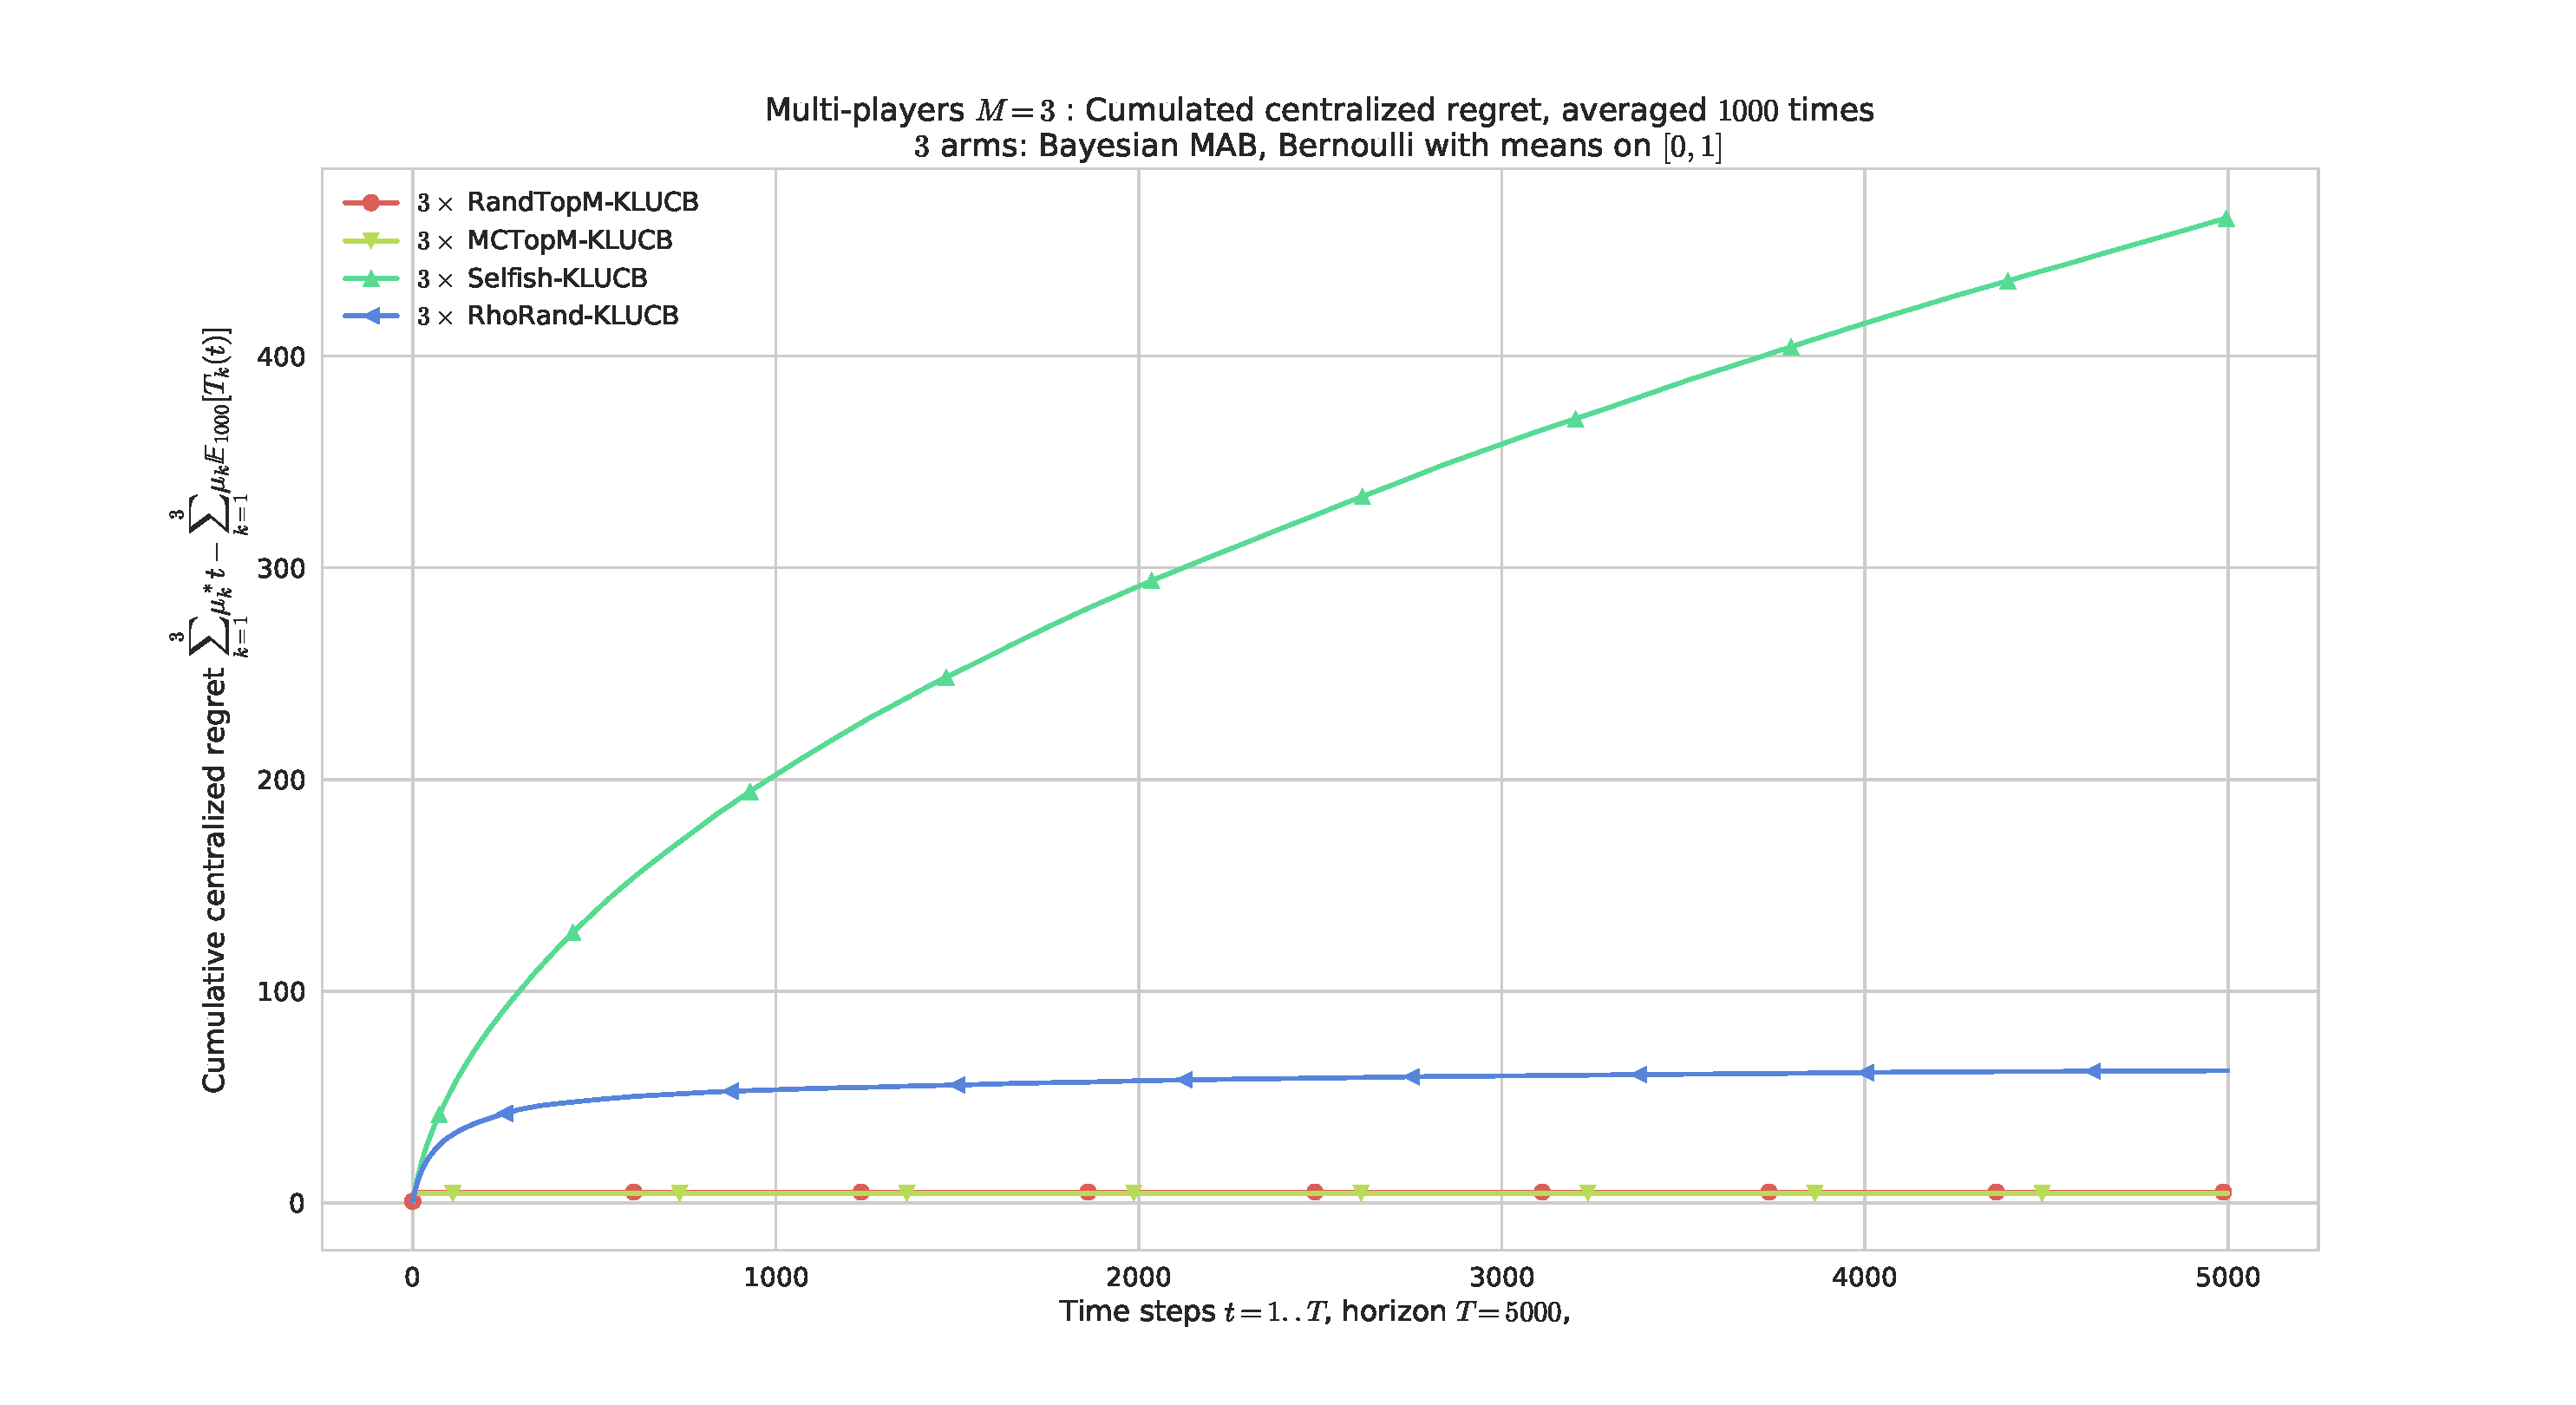
\includegraphics[width=1.05\textwidth]{MP__K3_M3_T5000_N1000__4_algos/all_RegretCentralized____env1-1_4683123079851881812.pdf}
%   % \end{subfigure}
%   \caption[Second failure case of \Selfish]{Regret, $M=2$ and $M=3$ players, $K=3$ arms, horizon $T=5000$, against $1000$ problems $\boldsymbol{\mu}$ uniformly sampled in $[0,1]^K$. \Selfish{} (top curve in \textcolor{darkgreen}{green}) clearly fails in such setting with small $K$.}
%   \label{fig:5:selfish_fail2}
%   % \vspace*{-15pt}  % XXX remove if problem
% \end{figure}

%
% Regular plots of centralized regrets
%

\begin{figure}[!t]
  \centering
  % \begin{subfigure}[!h]{1.00\textwidth}
      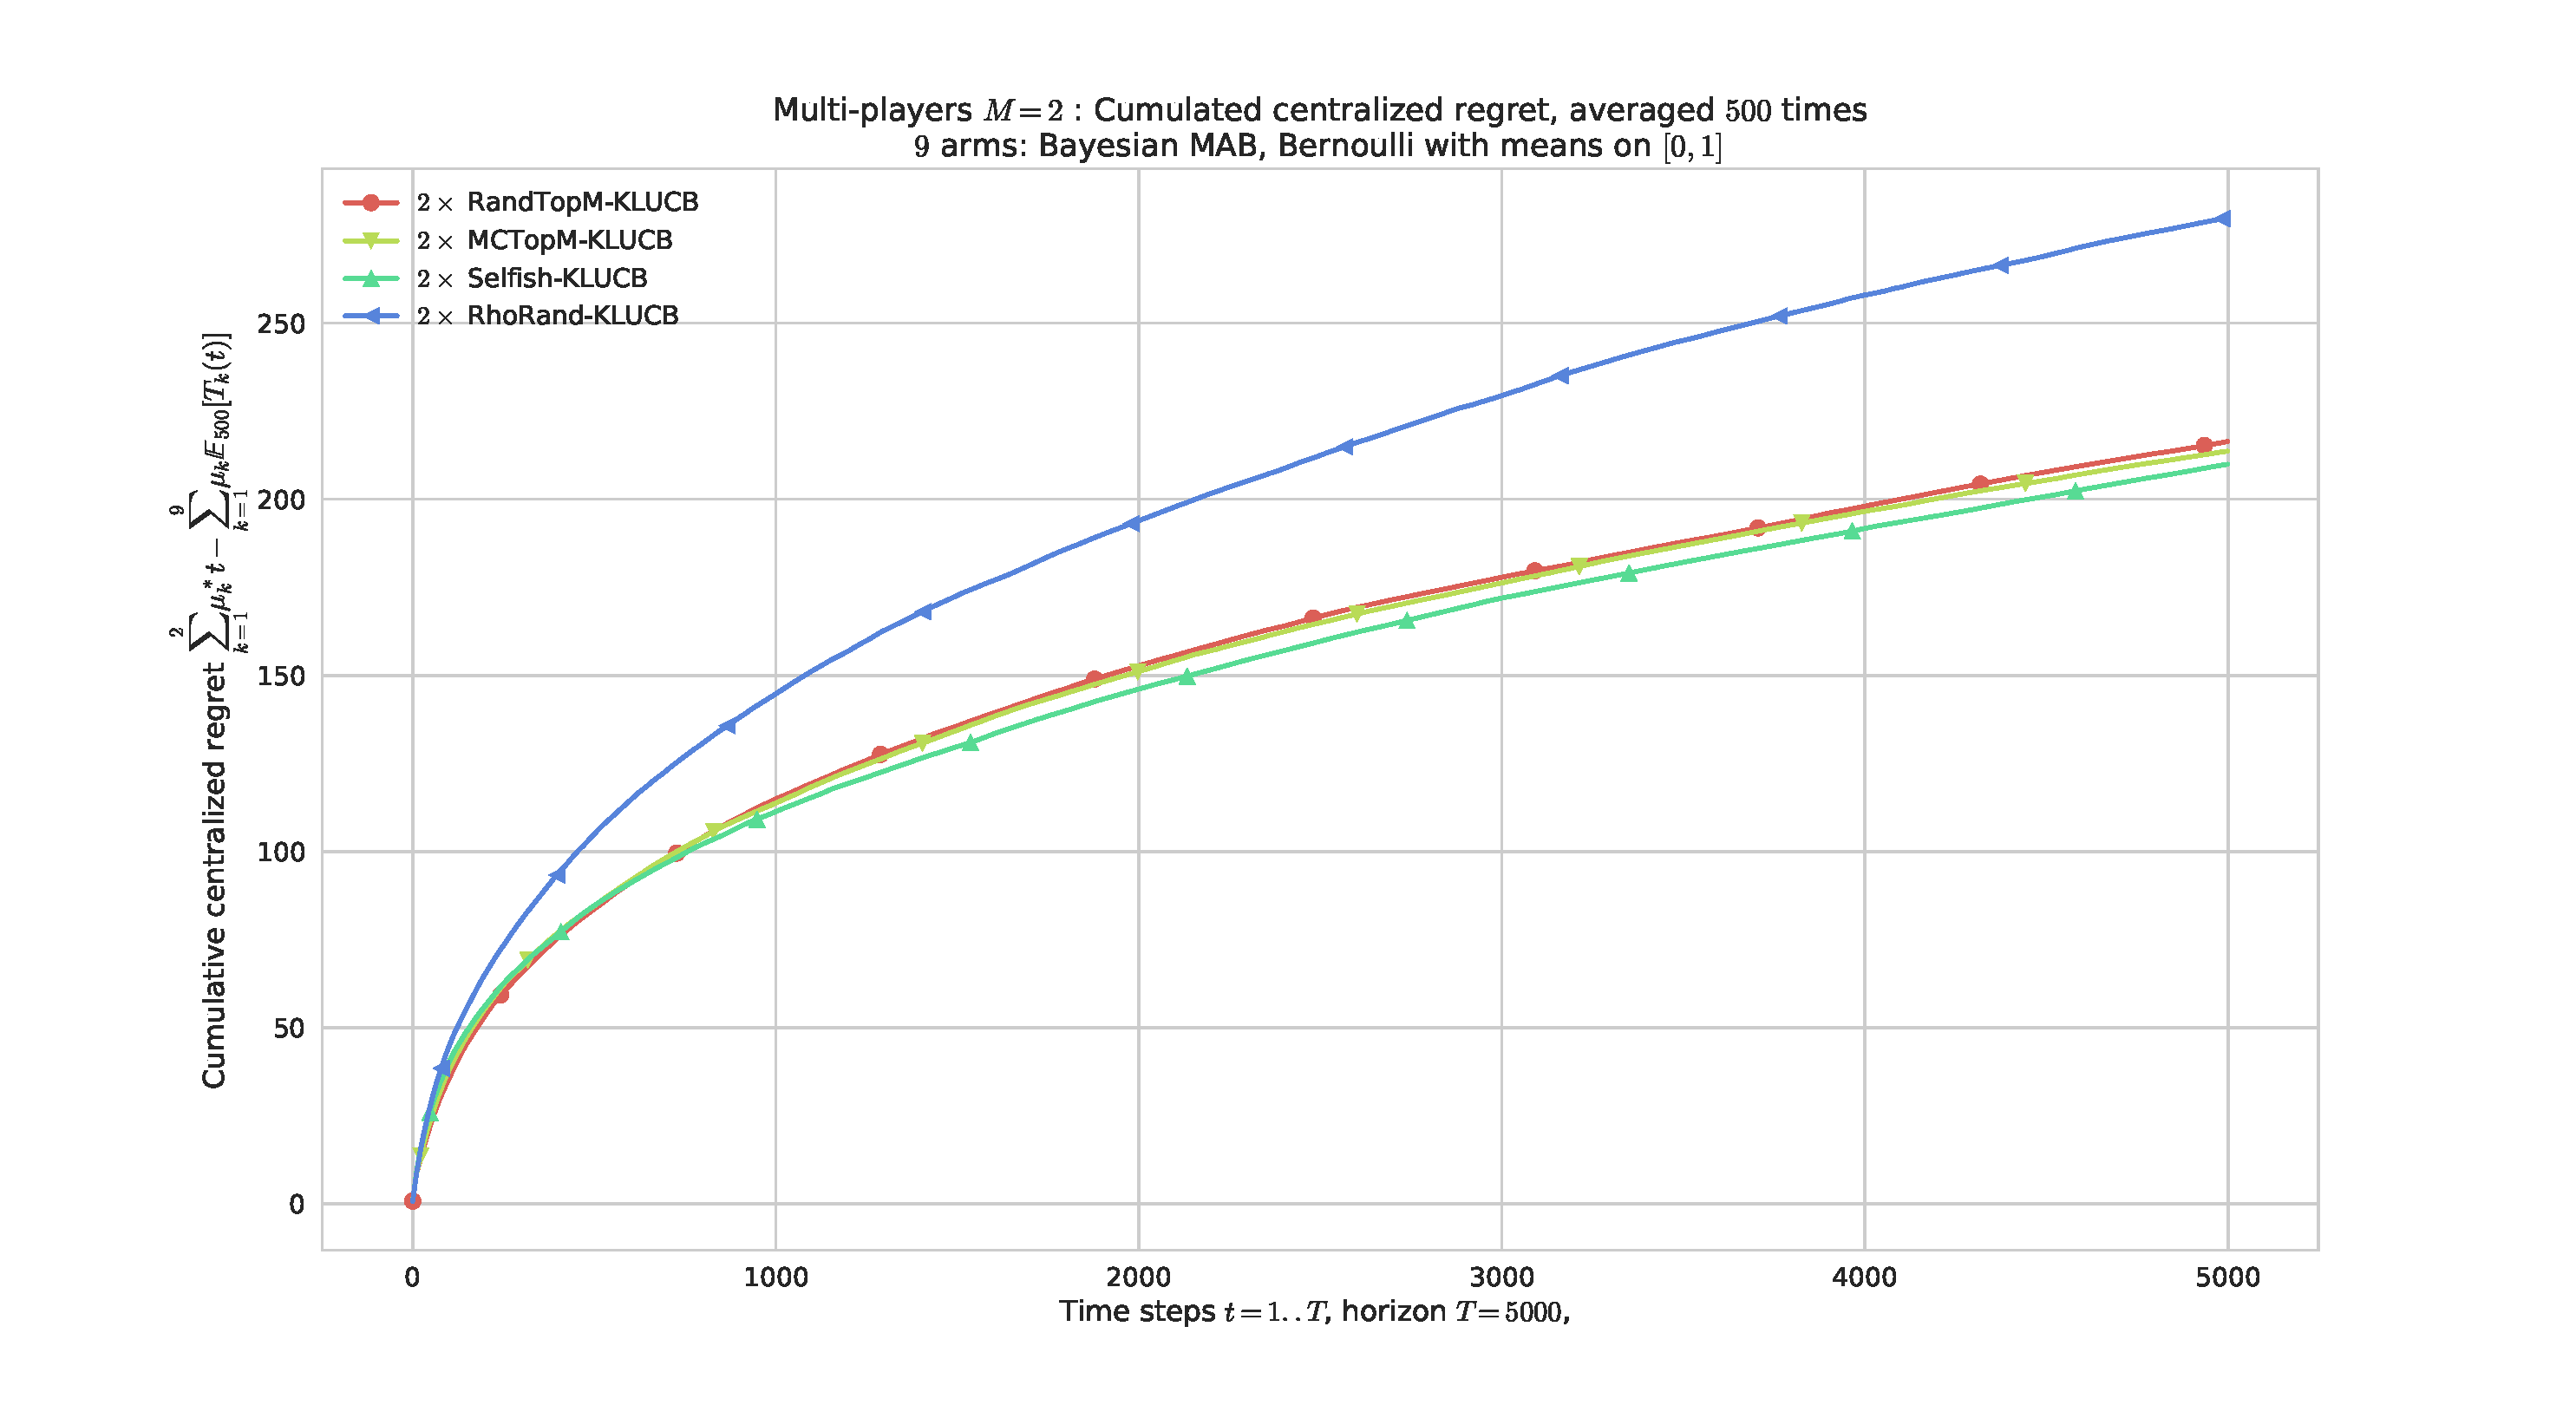
\includegraphics[width=1.10\textwidth]{MP__K9_M2_T5000_N500__4_algos/all_RegretCentralized____env1-1_3251433209347345969.pdf}
  % \end{subfigure}
  % ~
  \vspace{15pt}%  FIXME?
  % \begin{subfigure}[!h]{1.00\textwidth}
      % 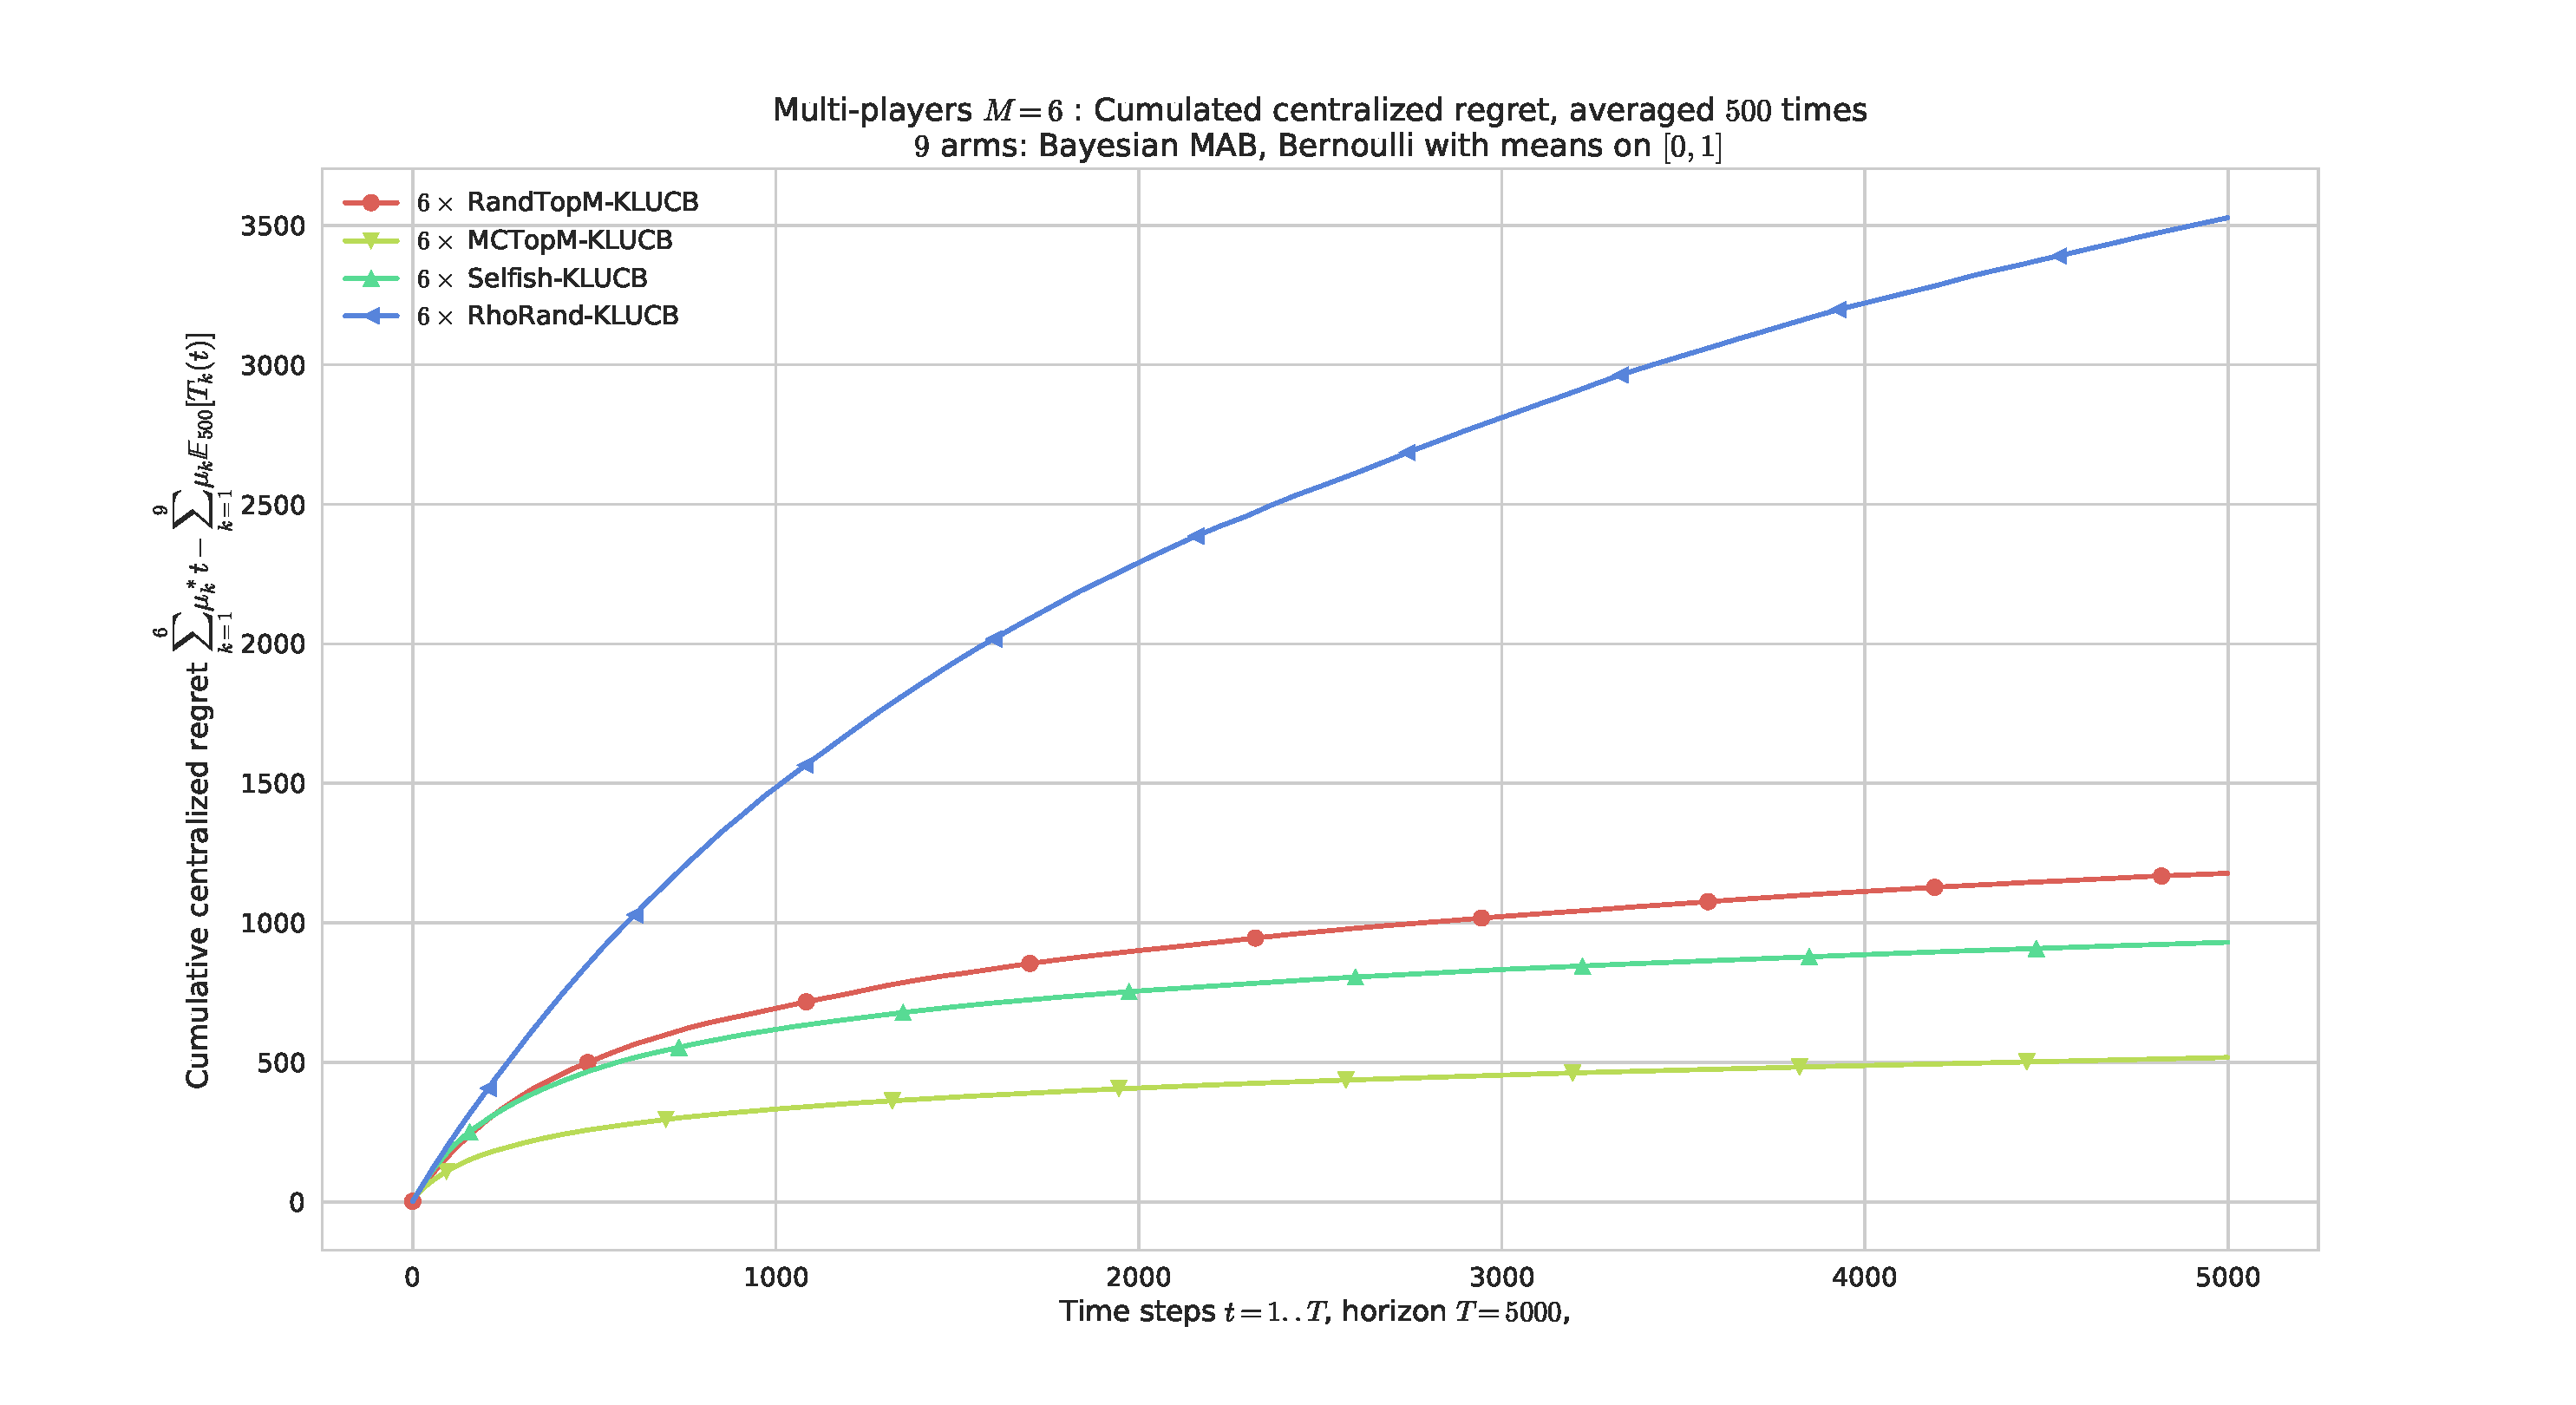
\includegraphics[width=1.00\textwidth]{MP__K9_M6_T5000_N500__4_algos/all_RegretCentralized____env1-1_8318947830261751207.pdf}
      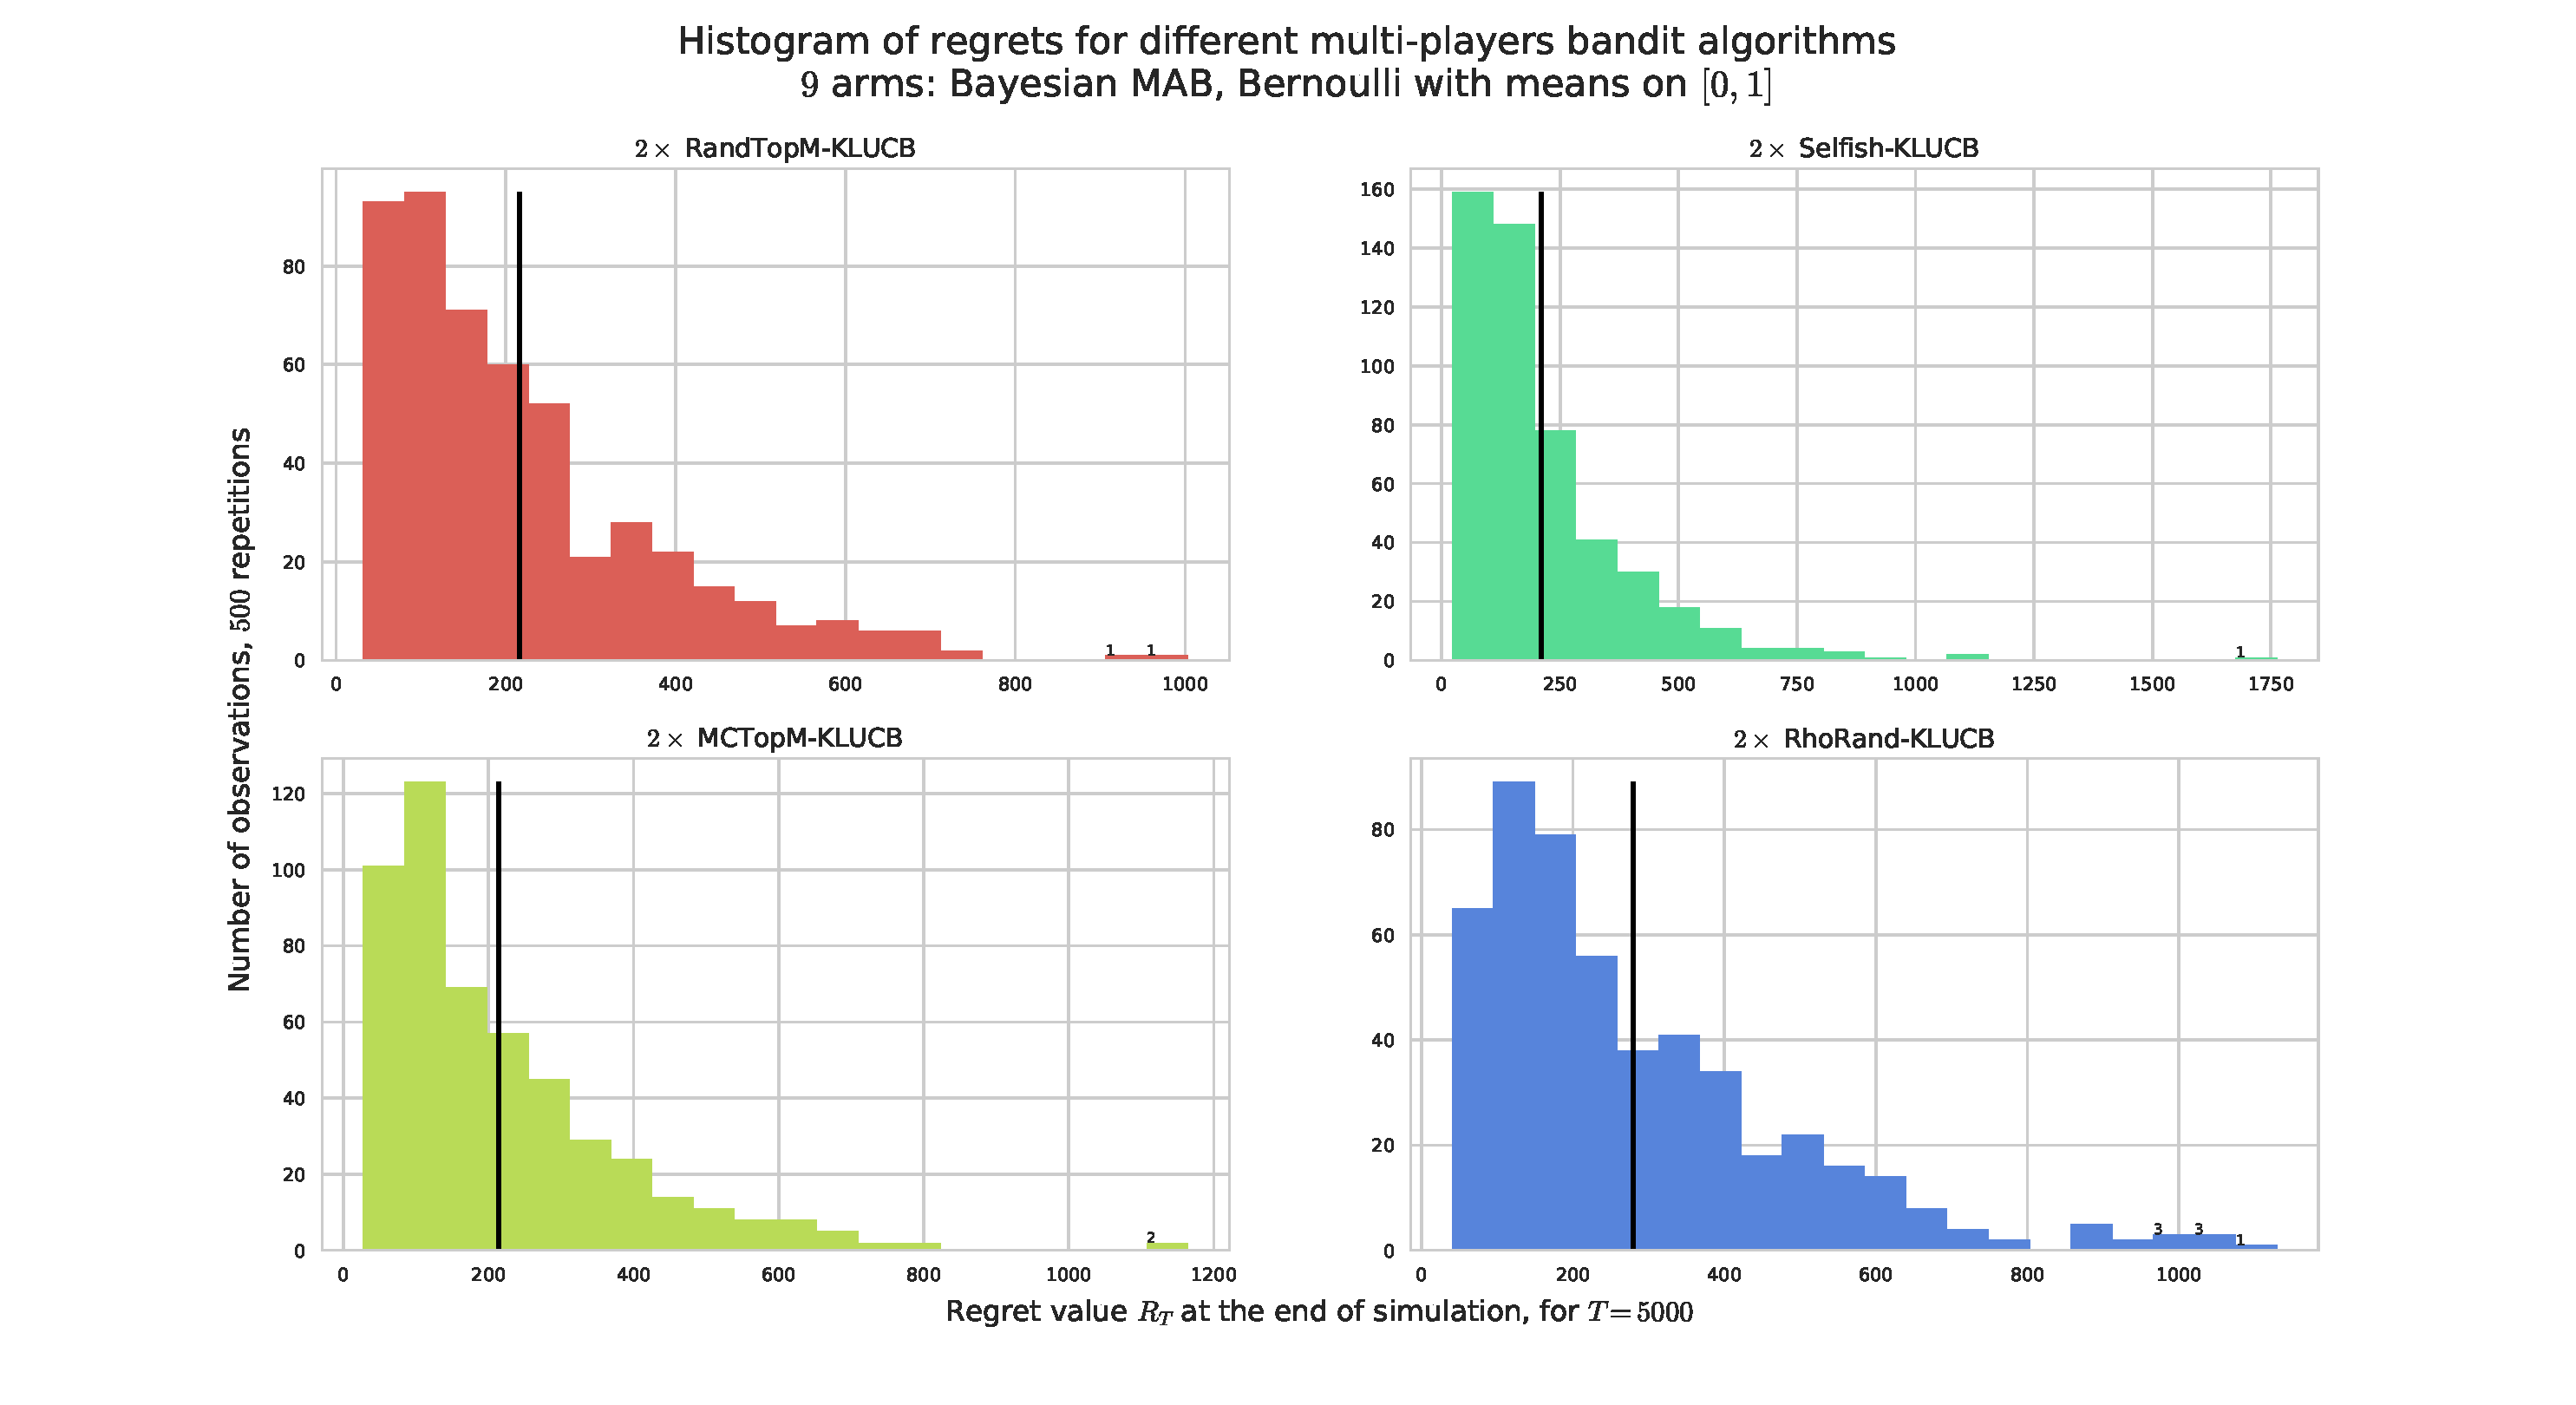
\includegraphics[width=1.10\textwidth]{MP__K9_M2_T5000_N500__4_algos/all_HistogramsRegret____env1-1_3251433209347345969.pdf}
  % \end{subfigure}
  \caption[Regret for $M=2$ players, $K=9$ arms, horizon $T=5000$, against $500$ problems $\boldsymbol{\mu}$ uniformly sampled.]{Regret for $M=2$ players, $K=9$ arms, horizon $T=5000$, against $500$ problems $\boldsymbol{\mu}$ uniformly sampled in $[0,1]^K$. \textcolor{blue}{\rhoRand{} (top blue)} is outperformed by the other algorithms (and the gain increases when $M$ increases), which all perform similarly in such configurations. Note that the (small) tail of the histograms come from complicated problems $\boldsymbol{\mu}$ and not failure cases.}
  \label{fig:5:MP__K9_M2_T5000_N500__4_algos__all_RegretCentralized__BayesianProblems}
  % \vspace*{-15pt}  % XXX remove if problem
\end{figure}


\begin{figure}[!t]
  \centering
  % \begin{subfigure}[!h]{1.00\textwidth}
      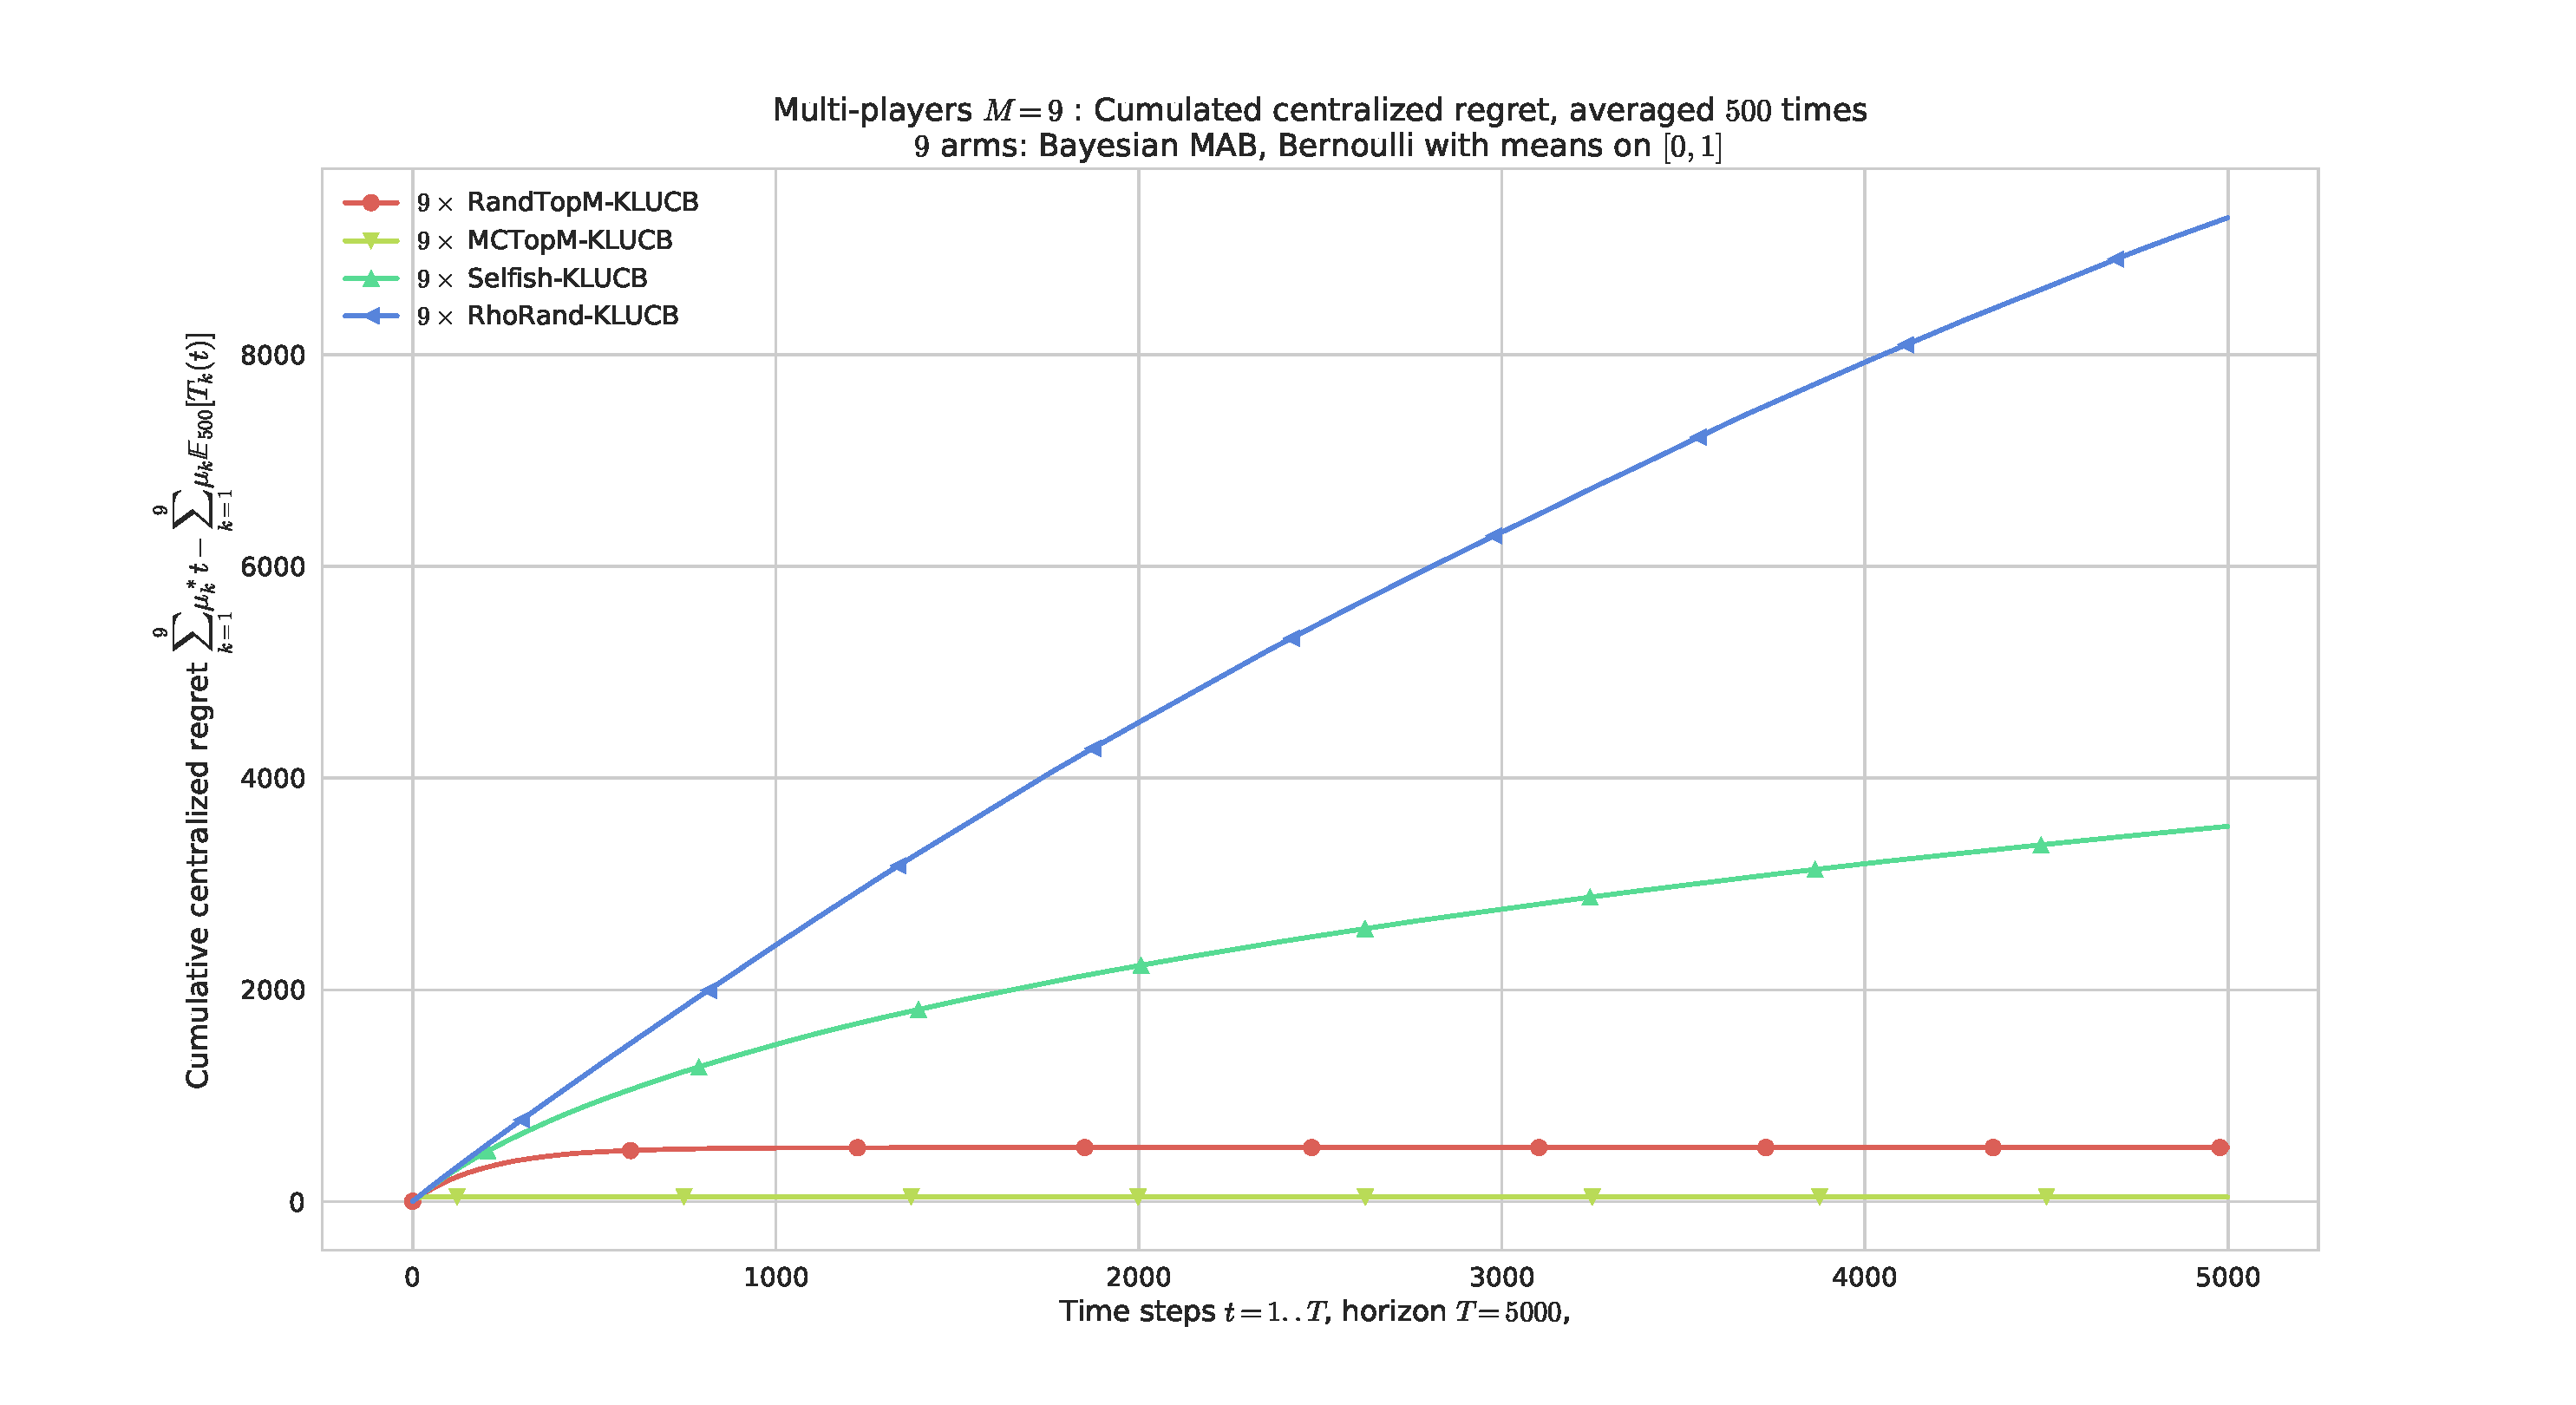
\includegraphics[width=1.10\textwidth]{MP__K9_M9_T5000_N500__4_algos/all_RegretCentralized____env1-1_3892966382091165662.pdf}
  % \end{subfigure}
  % ~
  \vspace{20pt}%  FIXME?
  % \begin{subfigure}[!h]{1.00\textwidth}
      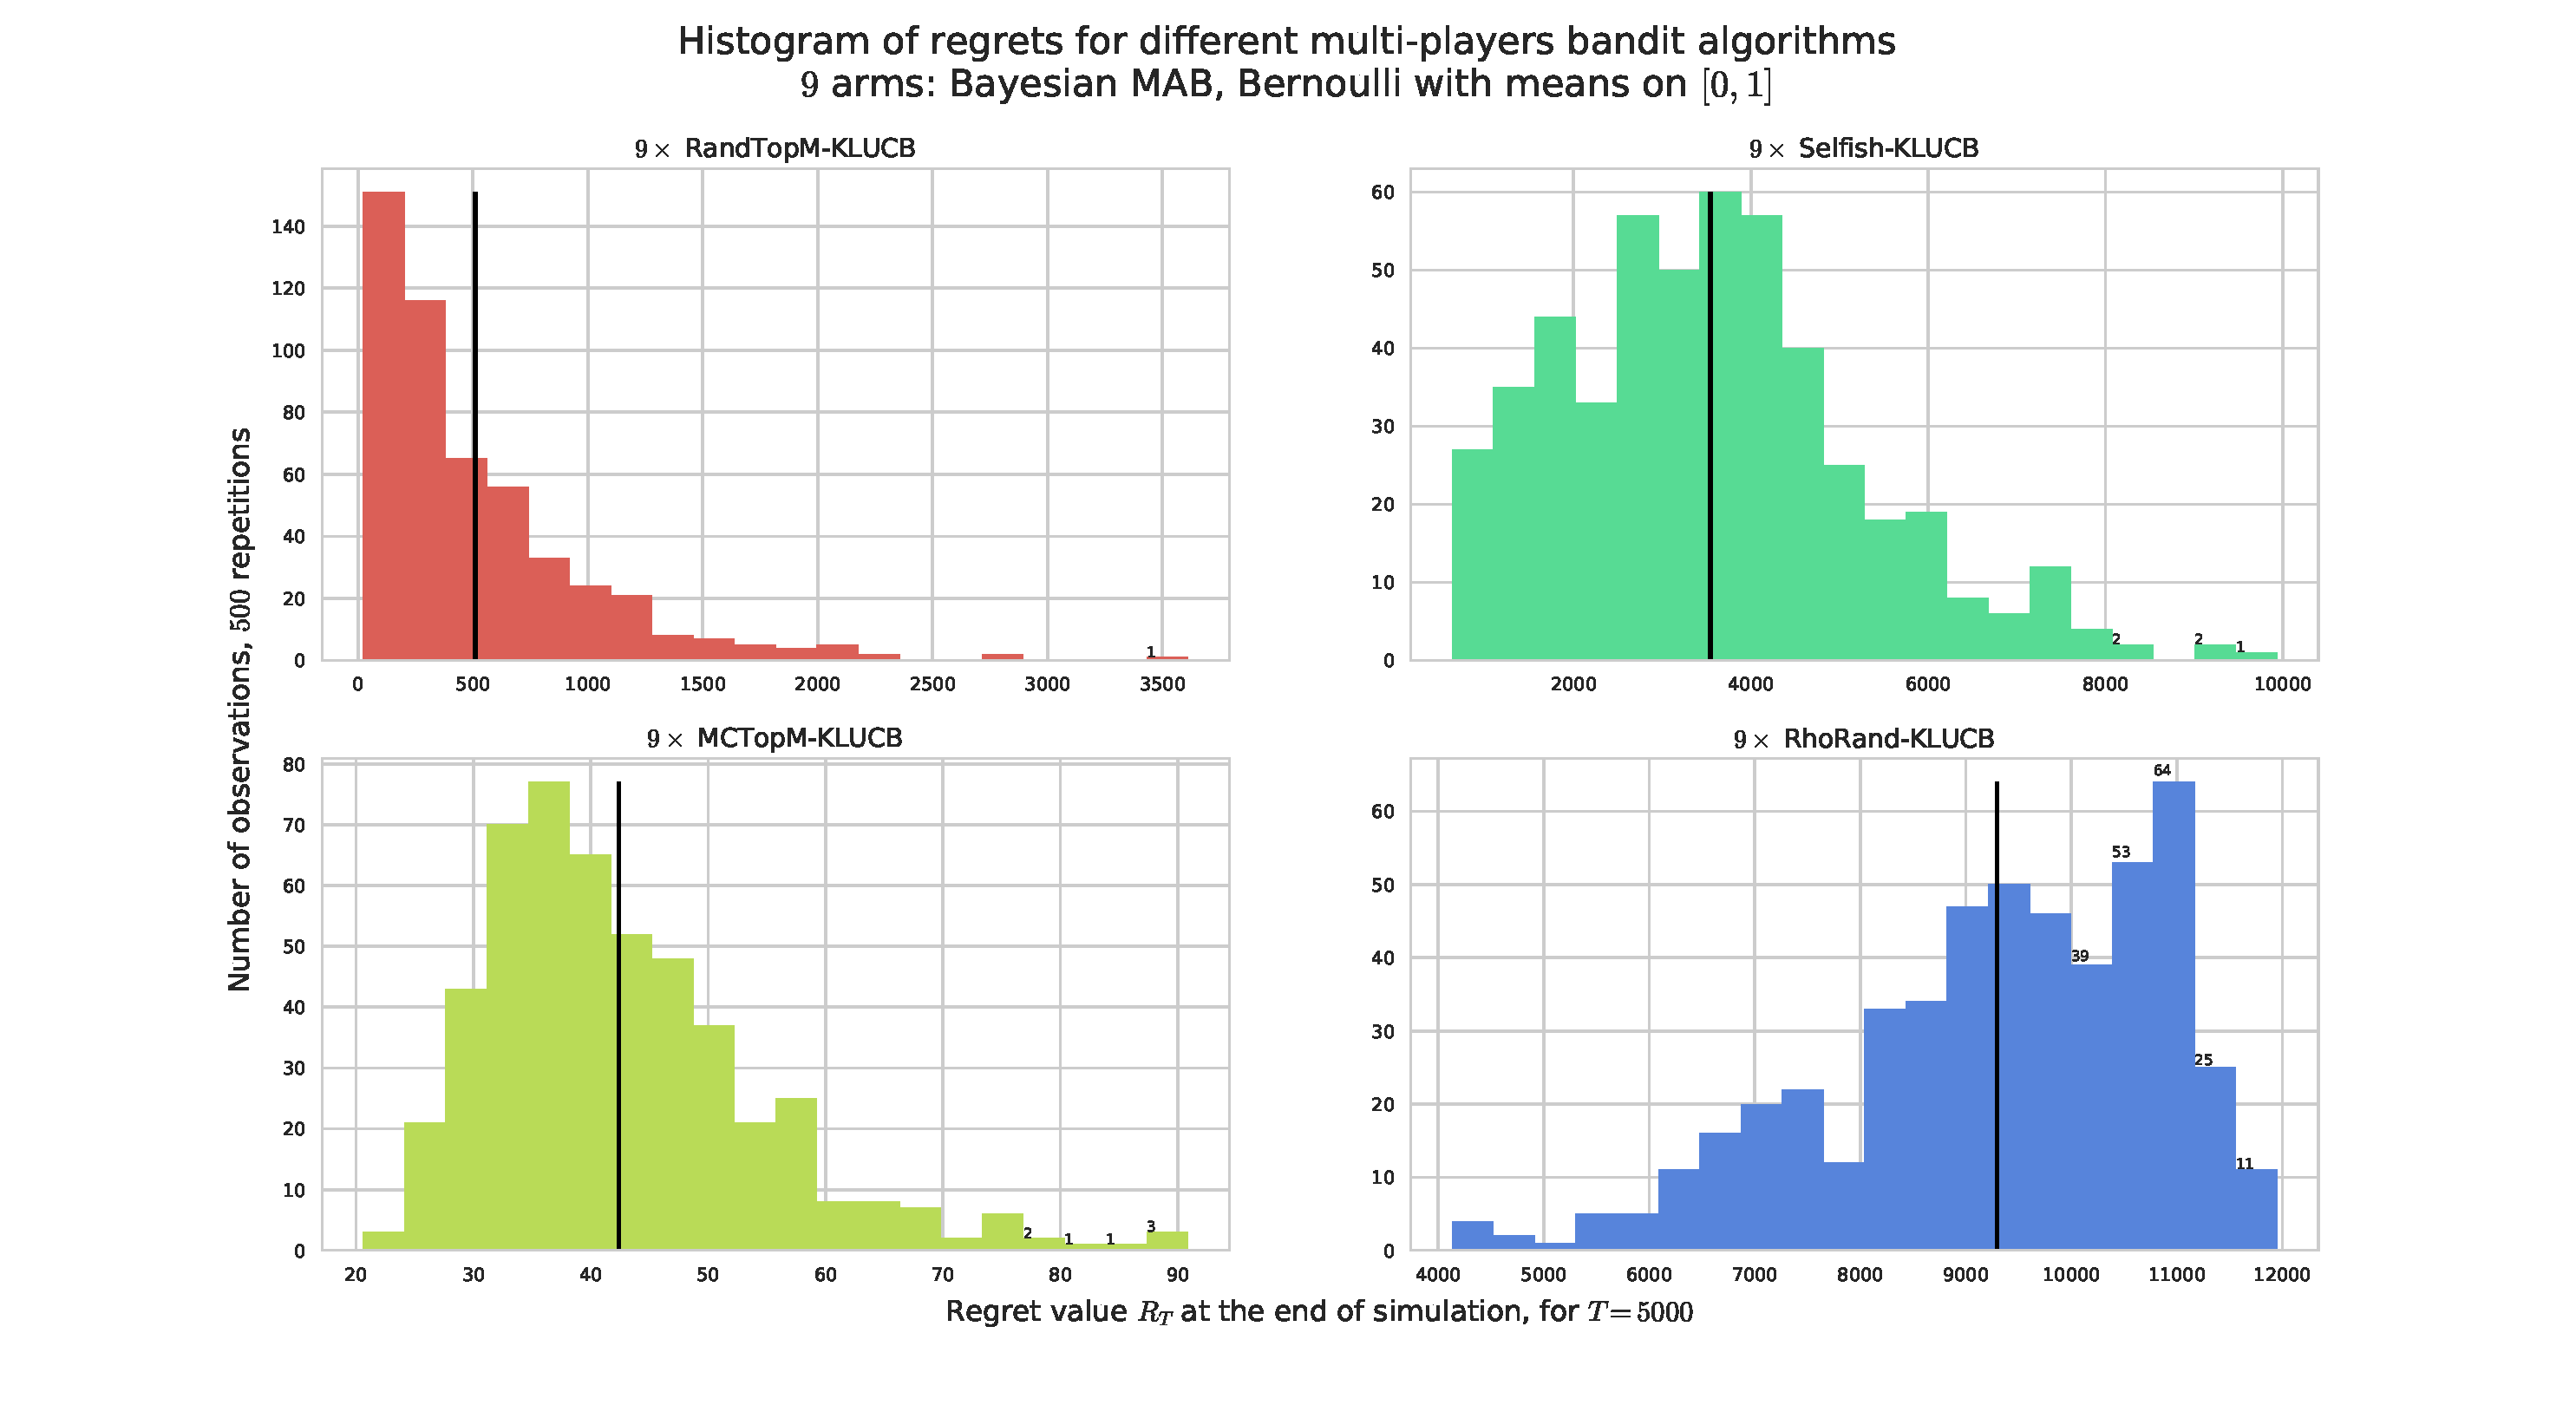
\includegraphics[width=1.10\textwidth]{MP__K9_M9_T5000_N500__4_algos/all_HistogramsRegret____env1-1_3892966382091165662.pdf}
  % \end{subfigure}
  \caption[Regret for $M=K=9$, horizon $T=5000$, against $500$ problems $\boldsymbol{\mu}$ uniformly sampled.]{Regret for $M=K=9$, horizon $T=5000$, against $500$ problems $\boldsymbol{\mu}$ uniformly sampled in $[0,1]^K$. This extreme case $M=K$ shows the drastic difference of behavior between \textcolor{red}{\RandTopM{} (red)} and \textcolor{lightgreen}{\MCTopM{} (light green)}, with constant regret, and \textcolor{blue}{\rhoRand{} (blue)} and \textcolor{darkgreen}{\Selfish{} (green)}, with large regret.}
  \label{fig:5:MP__K9_M9_T5000_N500__4_algos__all_HistogramsRegret}
  % \vspace*{-15pt}  % XXX remove if problem
\end{figure}


% Dynamic settings, when $M$ can change in time,
% were considered in the analysis of both
We also compared our algorithms to  %multi-players multi-armed bandits algorithms
with \MEGA{} \citep{Avner15} and \MusicalChair{} \citep{Rosenski16}, in the presence of sensing, \ie, observation model \modeldeux, for which they were developed.
Yet these two algorithms were found to both be very hard to use efficiently in practice, and we show in
% that were also proposed
%
Figure~\ref{fig:5:MP__K9_M3_T123456_N100__8_algos} that they perform poorly in comparison to \rhoRand, \RandTopM{} and \MCTopM.
%
\MEGA{} needs a careful tuning of \emph{five} parameters ($c$, $d$, $p_0$, $\alpha$ and $\beta$) to attain reasonable performances. No good guideline for tuning them is provided and using \emph{cross validation}, as suggested by \cite{Avner15},
can be considered out of the scope of \emph{online} sequential learning.
%In practice, on a fixed instance, the authors do not indicate how to select the parameters, even with a perfect knowledge of the parameters ($\boldsymbol{\mu}$ and $T$).
%
\MusicalChair{} consists of a random exploration phase of length $T_0$ after which the players quickly converge to orthogonal strategies targeting the $M$ best arms. With probability at least $1-\delta$, its regret is proven to be ``constant'' (of order $\log(1/\delta)$). The theoretical minimal value for $T_0$ depends on $\delta$, on the horizon $T$ and on a lower bound $\epsilon$ on the gap $\Delta = \mu^*_M - \mu^*_{M+1}$, and the practical tuning is hard too. %% which are both unavailable in our setting.


\paragraph{Uniformly sampled problems.}
%
Experiments with a different problem for each repetition,
that is uniformly sampled $\boldsymbol{\mu} \sim \cU([0,1]^K)$,
are also considered, in Figure~\ref{fig:5:MP__K9_M6_T5000_N500__4_algos__all_RegretCentralized__BayesianProblems} and \ref{fig:5:MP__K9_M2_T5000_N500__4_algos__all_RegretCentralized__BayesianProblems}.
This helps to check that no matter the \emph{complexity} of the considered problem (one measure of complexity being the constant in our lower bound),
\MCTopM{} performs similarly or better than all the other algorithms,
and \Selfish{} outperforms \rhoRand{} in most cases.
Figure~\ref{fig:5:MP__K9_M6_T5000_N500__4_algos__all_RegretCentralized__BayesianProblems} is a good example
of outstanding performances of \MCTopM{} and \Selfish{} in comparison to \rhoRand{}.
%
Empirically, our proposals were found to always outperform \rhoRand{}, and except for \Selfish{} that can fail badly on problems with small $K$,
we verified that \MCTopM{} outperforms the state-of-the-art algorithms in many different problems, and is more and more efficient as $M$ and $K$ grows.

Note that more numerical experiments were conducted for the article \cite{Besson2018ALT}, and in particular the last pages of the paper show more figures, in other settings.

% \begin{framed}
%   \textcolor{red}{\textbf{FIXME}}
%   Je ne sais pas trop comment inclure toutes ces figures ici, avant la dernière section où je parle des extensions de nos modèles.
%   J'aimerai bien avoir quelques pages simplement remplies des figures, sans avoir le texte de Section~\ref{sec:5:literatureReviewOtherModels} qui commence au milieu...
%   Une idée ?
% \end{framed}


% ----------------------------------------------------------------------------
% \subsection{Some future work on SMPyBandits}
\paragraph{Reproducibility.}

The experiments in this chapter use our library SMPyBandits,
and the page \href{https://SMPyBandits.GitHub.io/MultiPlayers.html}{\texttt{SMPyBandits.GitHub.io/MultiPlayers.html}} gives instructions to reproduce them.
